\documentclass{beamer}

\mode<presentation> {


  %\usetheme{default}
  %\usetheme{AnnArbor}
  %\usetheme{Antibes}
  %\usetheme{Bergen}
  %\usetheme{Berkeley}
  %\usetheme{Berlin}
  %\usetheme{Boadilla}
  %\usetheme{CambridgeUS}
  %\usetheme{Copenhagen}
  %\usetheme{Darmstadt}
  %\usetheme{Dresden}
  %\usetheme{Frankfurt}
  %\usetheme{Goettingen}
  %\usetheme{Hannover}
  %\usetheme{Ilmenau}
  %\usetheme{JuanLesPins}
  %\usetheme{Luebeck}
  \usetheme{Madrid}
  %\usetheme{Malmoe}
  %\usetheme{Marburg}
  %\usetheme{Montpellier}
  %\usetheme{PaloAlto}
  %\usetheme{Pittsburgh}
  %\usetheme{Rochester}
  %\usetheme{Singapore}
  %\usetheme{Szeged}
  %\usetheme{Warsaw}


  %\usecolortheme{albatross}
  %\usecolortheme{beaver}
  %\usecolortheme{beetle}
  %\usecolortheme{crane}
  %\usecolortheme{dolphin}
  %\usecolortheme{dove}
  %\usecolortheme{fly}
  %\usecolortheme{lily}
  %\usecolortheme{orchid}
  %\usecolortheme{rose}
  %\usecolortheme{seagull}
  %\usecolortheme{seahorse}
  %\usecolortheme{whale}
  %\usecolortheme{wolverine}

  %\setbeamertemplate{footline} % To remove the footer line in all slides uncomment this line
  %\setbeamertemplate{footline}[page number] % To replace the footer line in all slides with a simple slide count uncomment this line

  %\setbeamertemplate{navigation symbols}{} % To remove the navigation symbols from the bottom of all slides uncomment this line
}

\usepackage{graphicx}
%\usepackage{booktabs}
\usepackage{wrapfig}
\usepackage{float}
\usepackage{sidecap}
\usepackage{caption}
\usepackage{subcaption}
\usepackage{multicol}
%\usepackage{lmodern}
%\usepackage{textcomp}
%\usepackage{hyperref}
%\usepackage{tabular}
\usepackage{array}
\usepackage{amsmath}
\usepackage{mathtools}
\usepackage{slashed}
\usepackage{siunitx}
%% \usepackage{amssymb}
%% \usepackage{enumitem}
%% \usepackage{lipsum}
%% \usepackage[3D]{movie15}
\usepackage{tcolorbox}
\graphicspath{{figures/}}


\title[Multiplicity \& Charge Ratio]{Multiplicity of muon in 2\,m\,$\times$\,2\,m detector and charge ratio of cosmic muon at Madurai}
\author[Suryanarayan]{Suryanarayan Mondal}
\institute[INO] {
  \begin{figure}[htbp]
    \center
    \vspace{-15pt}
    
\includegraphics[width=0.26\linewidth]{hbni_logo.png}
  \end{figure}
  \small{Viva-voce towards award of PhD degree from HBNI}\\
  \small{Enrollment No: PHYS01201404020}\\
  \small{Supervisor: Prof. Prashant Shukla}
}
\date{June 28, 2021}


\begin{document}

\begin{frame}
  \titlepage
\end{frame}

\begin{frame}
  \frametitle{INO-ICAL experiment}
  \begin{columns}
    \begin{column}{0.5\textwidth}
      \begin{itemize}
      \item INO-ICAL with its 50\,kton magnetised iron calorimeter
        is a proposed underground experiment to primarily
        measure sign of the  $\Delta m_{32}^{2}$ mass-squared
        difference, through matter effects along with
        the oscillation in the $\nu$ and $\bar{\nu}$.
      \item About 30000 glass Resistive Plate Chamber (RPC) of size
        2\,m\,$\times$\,2\,m will be used as sensitive detectors
        to measure energy and direction of the particles
        produced in the interaction of neutrinos with iron.
      \end{itemize}
    \end{column}
    \begin{column}{0.5\textwidth}
      \begin{figure}
        \begin{center}
          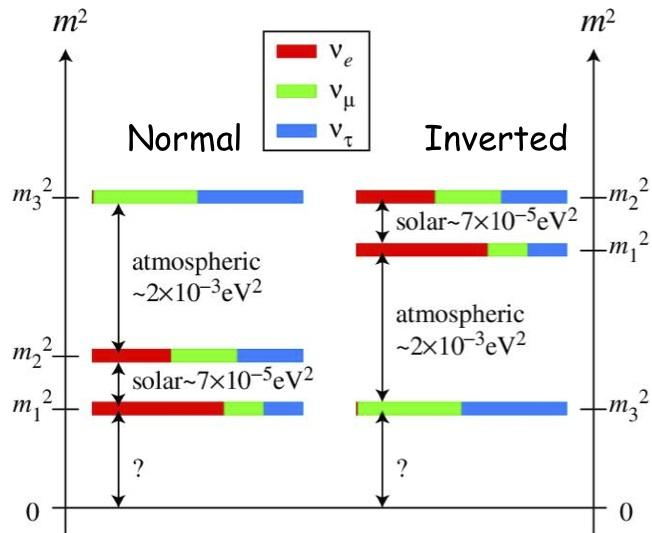
\includegraphics[width=0.7\linewidth]{p11.jpg}\\
          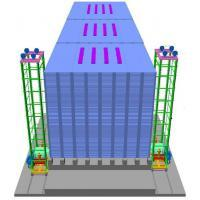
\includegraphics[width=0.7\linewidth]{inoical.jpg}
        \end{center}
      \end{figure} 
    \end{column}
  \end{columns}
\end{frame}

\begin{frame}
  \frametitle{Motivation of thesis}
  \begin{tcolorbox}
    To perform neutrino oscillation studies using atmospheric
    neutrinos, the knowledge of neutrino flux at the project site
    is essential.
    Many prototype detectors are built and also proposed
    near to the location of the project site to better
    understand the flux of the atmospheric muons along with
    the R\&D on the RPCs, magnet and electronics.
  \end{tcolorbox}
  \vspace{1cm}
  \colorbox{gray!40}{\begin{minipage}{0.4\textwidth}%% {17.5cm}
      \bf {Flow of Presentation} 
  \end{minipage}}
  \begin{minipage}{1.0\textwidth}
    \vspace{5pt}
    \begin{enumerate}
    \item Leak Test of RPCs
    \item Multiplicity of Particles
    \item Muon Charge Ratio
    \end{enumerate} 
  \end{minipage}
\end{frame}

\begin{frame}
  \frametitle{Active Detector: Resistive Plate Chamber}
  \vspace*{-7pt}
  \begin{itemize} \itemsep -1pt
  \item The RPC gaps are made of 3\,mm thick glass plates with 2\,mm
    gas gap.
  \item The mixture of R134a (95.2\%), iso-C$_4$H$_{10}$ (4.2\%)
    and SF$_6$ (0.3\%) is the target medium of the RPCs.
  \item The RPCs are applied $\pm$5\,kV via the graphite coating on the
    opposite sides of the glass plates.
  \item The avalanche formed by the passing particles are sensed
    using orthogonal copper pickup strips of pitch 3\,cm.
  \end{itemize}
  \vspace*{-8pt}
  \begin{figure}[h!]
    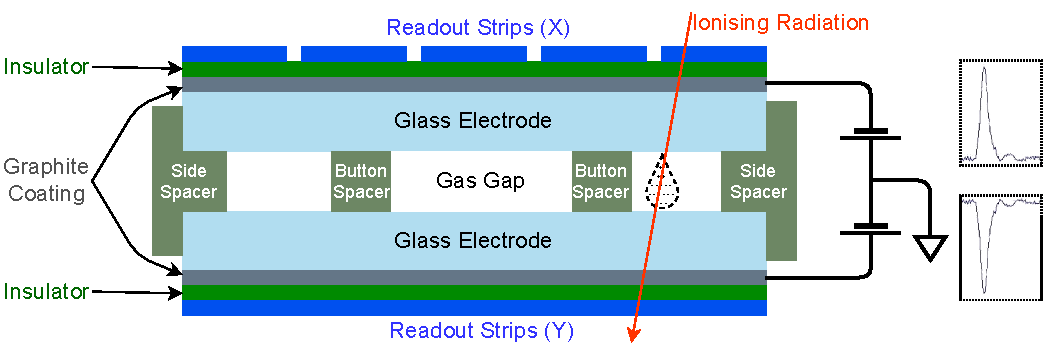
\includegraphics[width=0.9\textwidth]{basic_rpc.pdf}
  \end{figure}
  \vspace*{-12pt}
  \begin{itemize} %% \itemsep -1pt
  \item The charged particles, mostly cosmic ray muons, create curved
    trajectory in the detector due to magnetic field.
  \end{itemize}
\end{frame}

\begin{frame}
  \frametitle{Leak Test of RPC}
  \vspace{-10pt}
  \begin{itemize} \itemsep -1pt
  \item The RPCs are pressurised up-to 45mmWC above atmosphere and
    then sealed.
  \end{itemize}
  \vspace{-8pt}
  \begin{figure}[h]%% [!h]
    \centering
    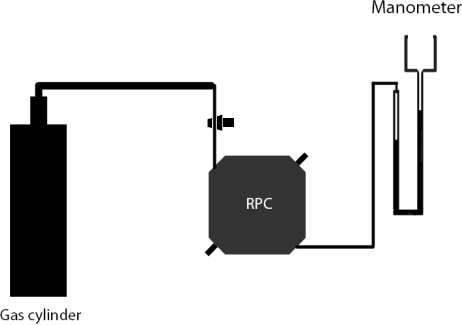
\includegraphics[width=0.5\textwidth]{test_rpc.png}
    \hspace{20pt}
    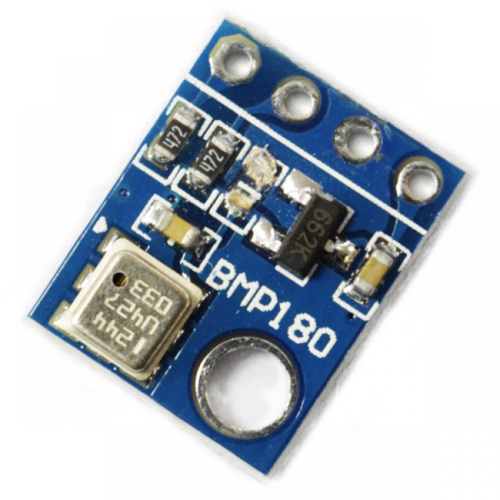
\includegraphics[width=0.25\textwidth]{bmp-180.png}
  \end{figure}
  \vspace{-12pt}
  \begin{itemize} \itemsep -1pt
  \item Room temperature, atmospheric pressure and pressure inside
    RPCs are monitored independently and recorded in each 3-5 sec.
  \item Instead of using conventional differential pressure sensors,
    absolute pressure sensor (BMP180) is used to record data.
  \item Two setups, wired and wireless, are designed to test
    multiple RPCs at the same time without removing them from the
    storage.
  \end{itemize}
\end{frame}

\begin{frame}
  \frametitle{Scheme of Wired Leak Test Setup}
  \begin{figure}[!h]
    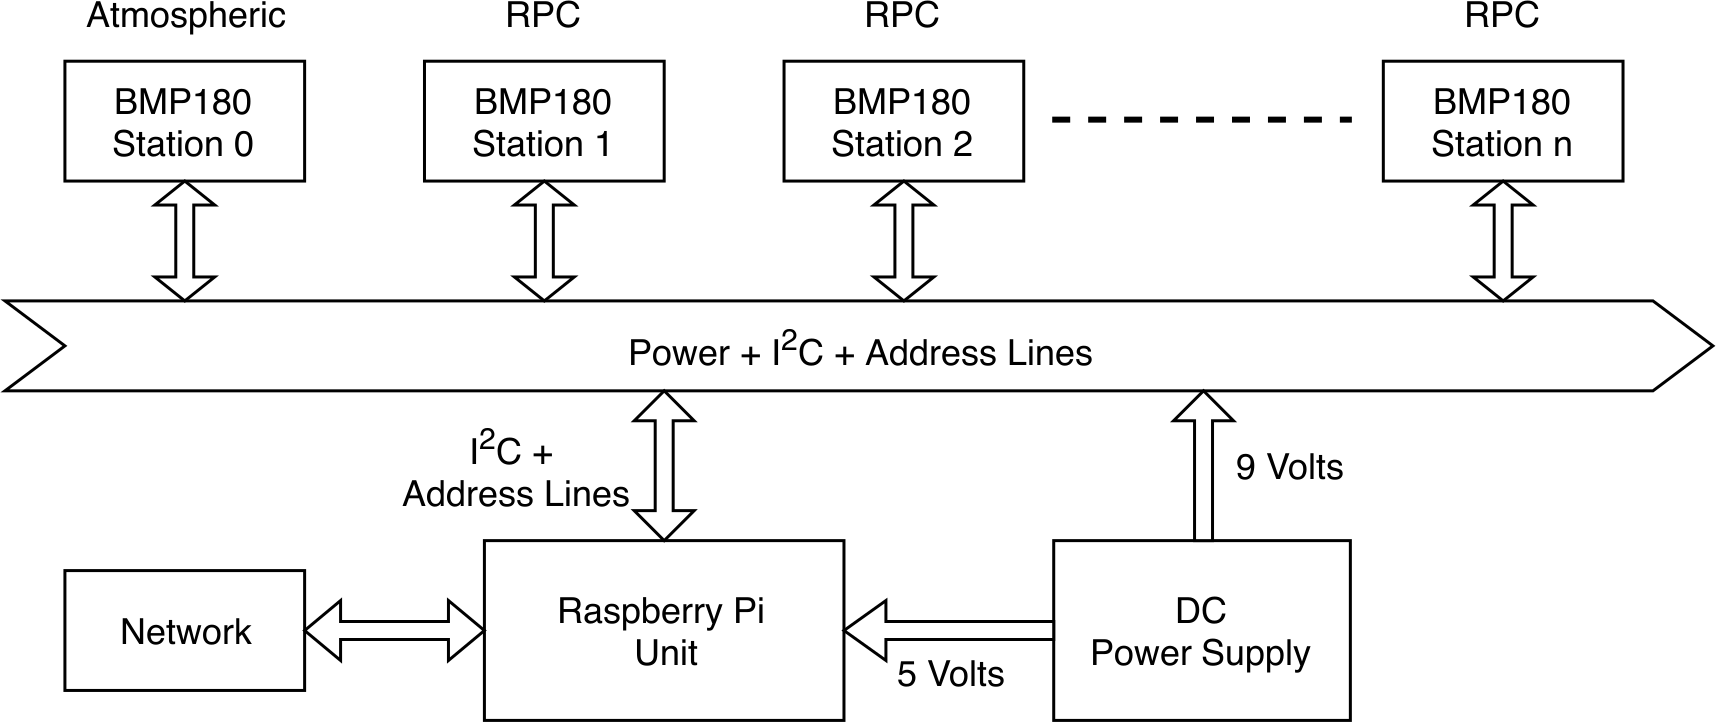
\includegraphics[width=0.8\textwidth]{leaktest_setup.png}\\
    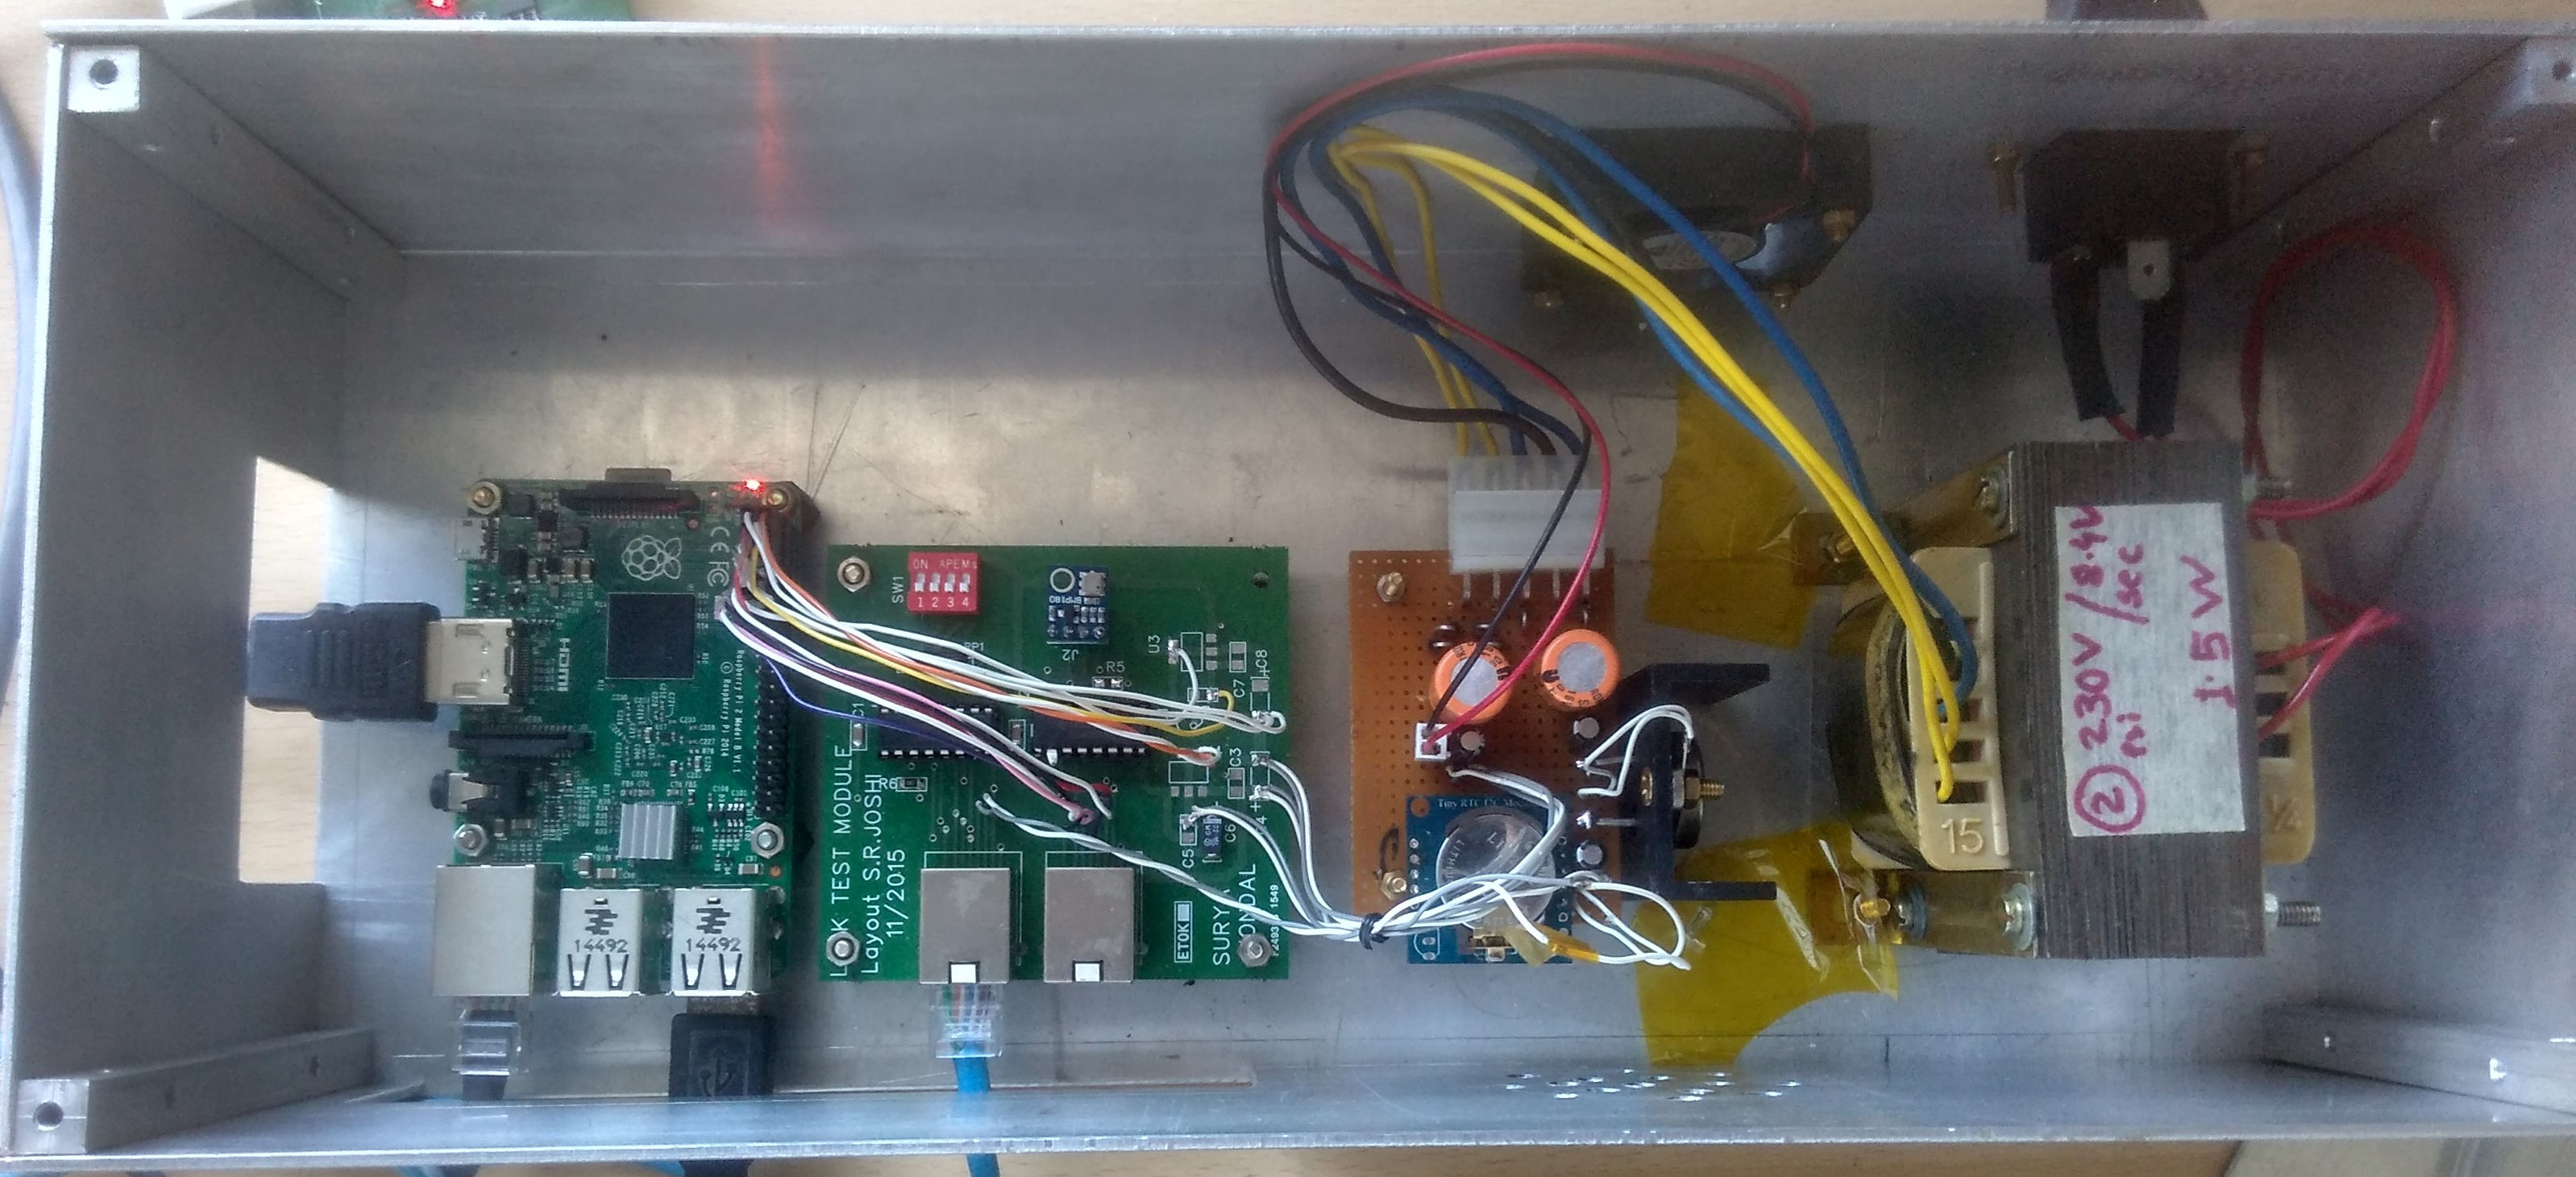
\includegraphics[width=0.65\textwidth]{pc2.jpg}
    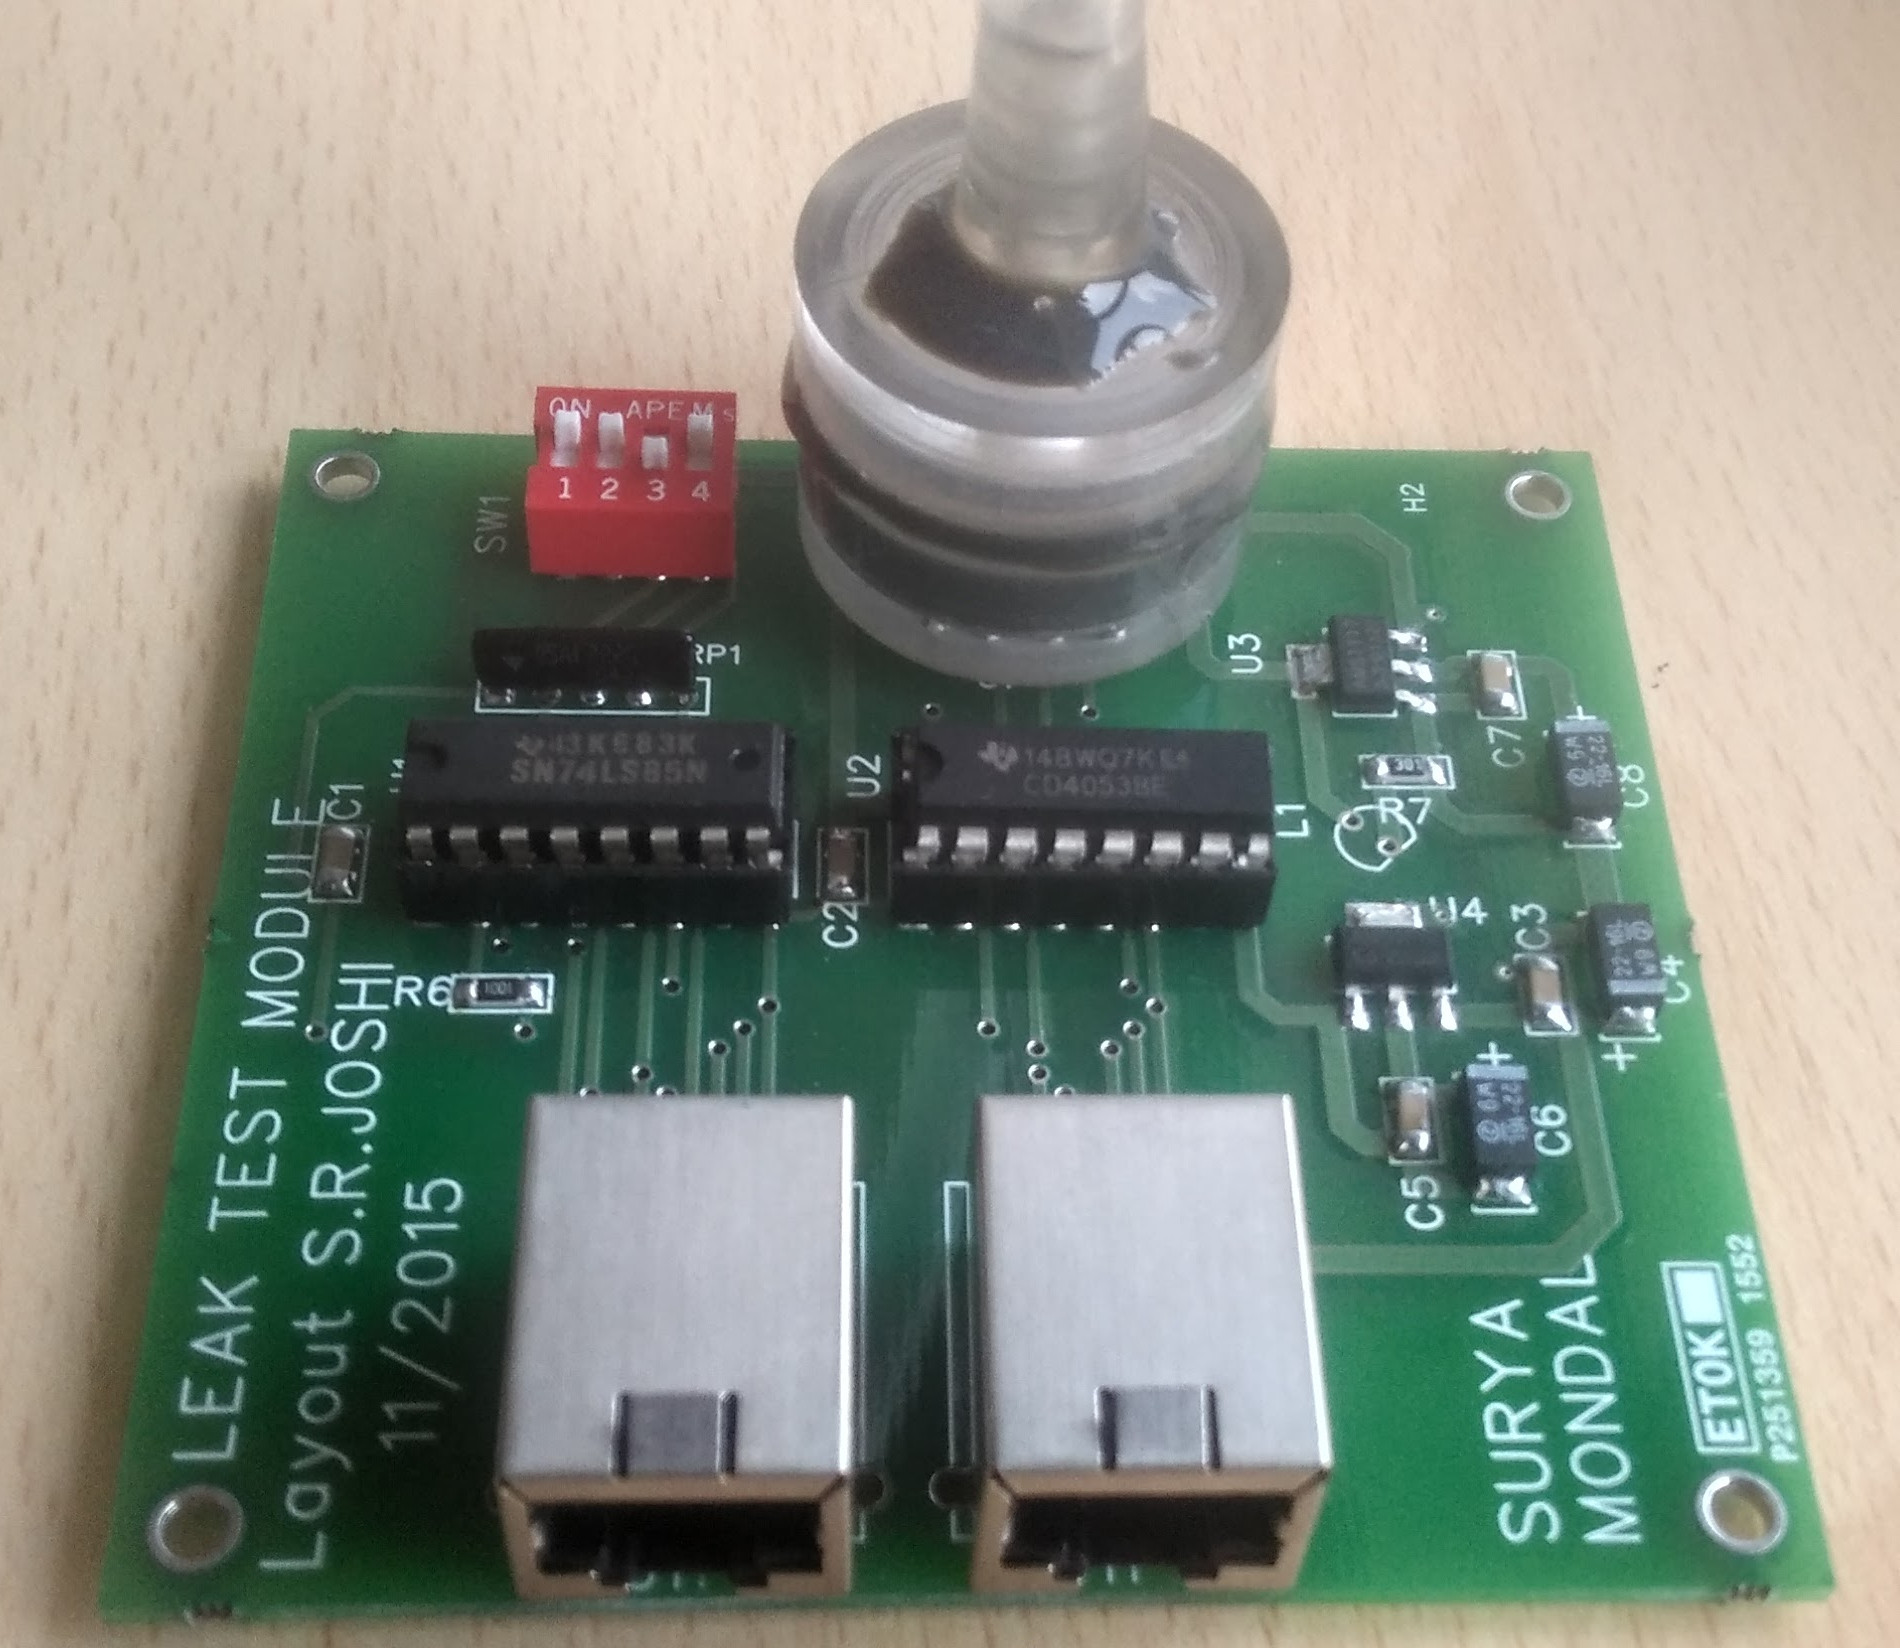
\includegraphics[width=0.34\textwidth]{pc3.jpg}
  \end{figure}
\end{frame}

\begin{frame}
  \frametitle{Scheme of Wireless Leak Test Setup}
  \begin{figure}[!h]
    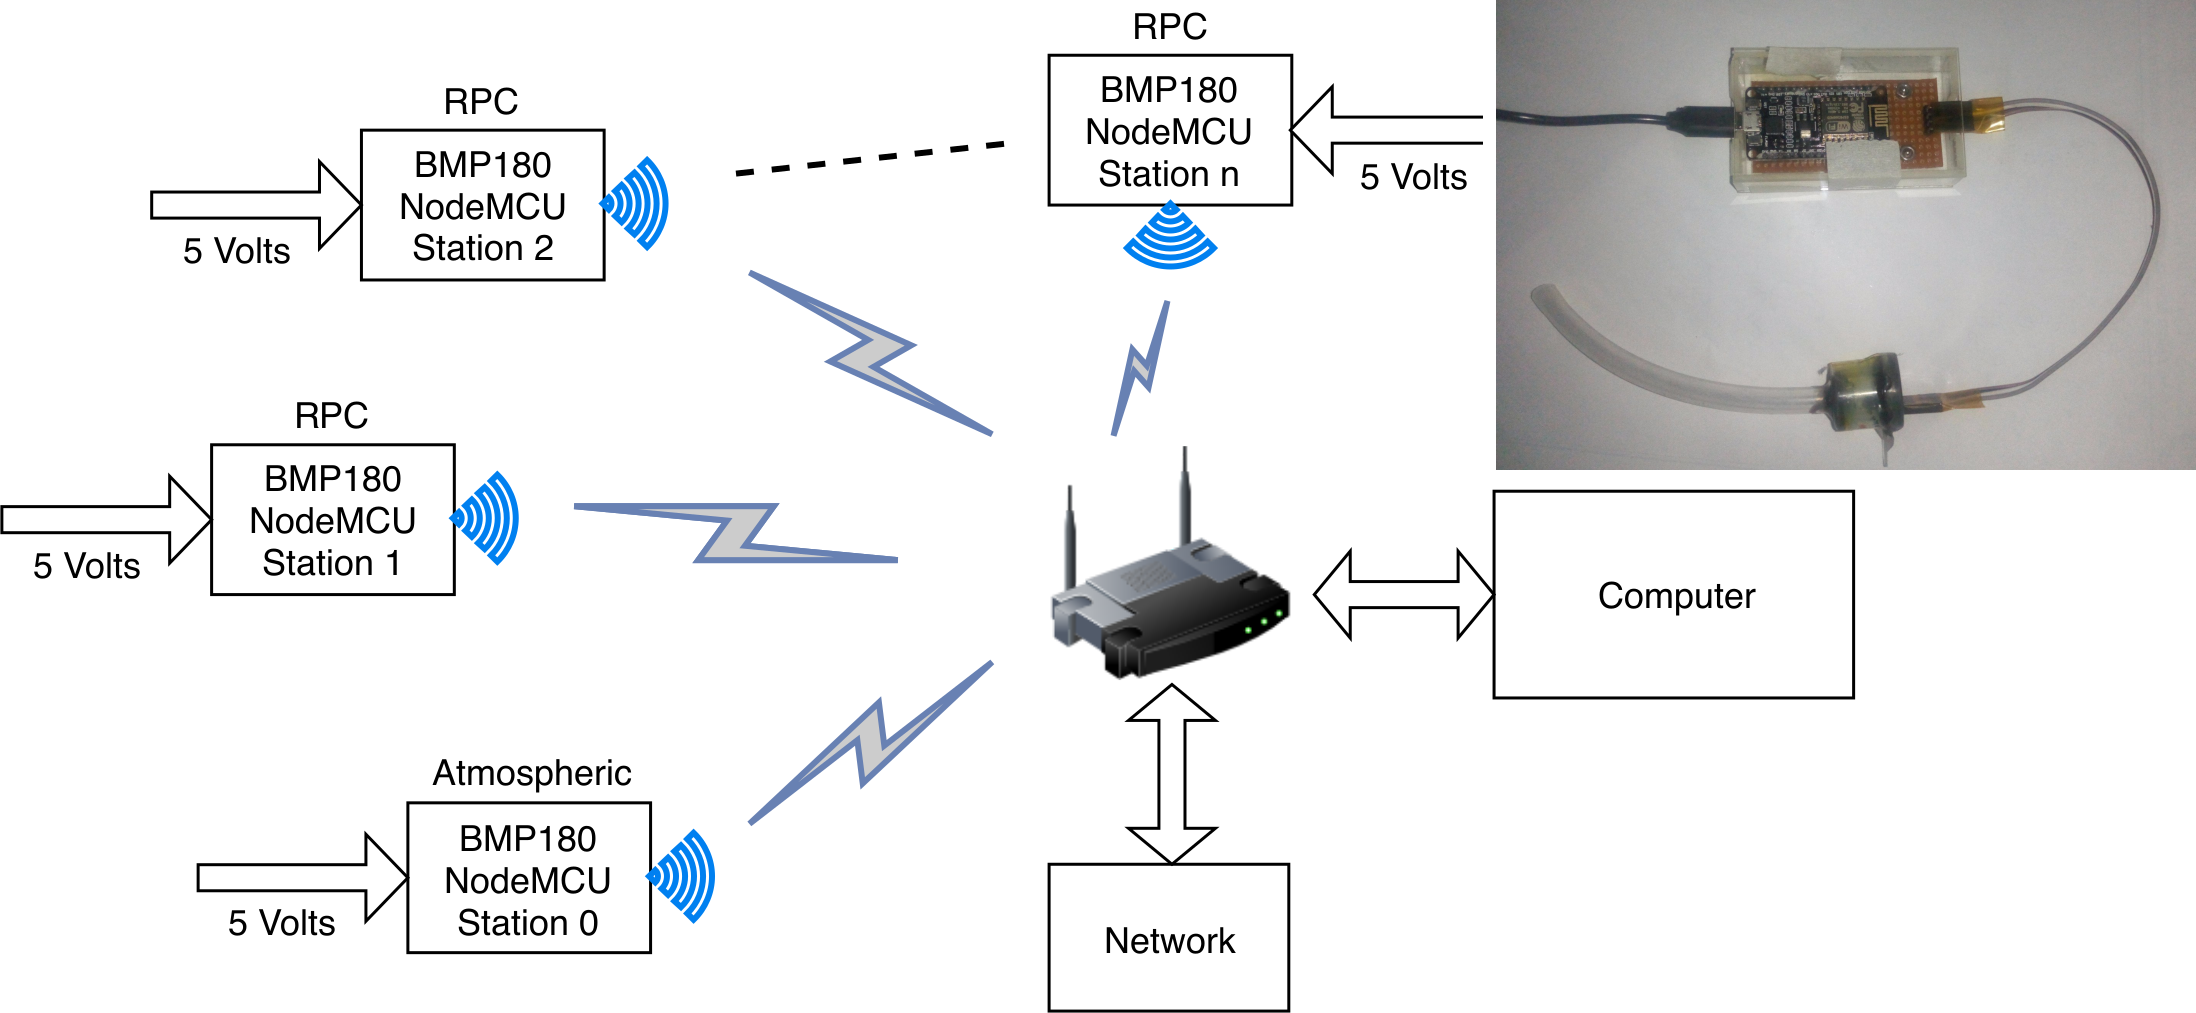
\includegraphics[width=0.9\textwidth]{leaktest_setup_wifi_all.png}
  \end{figure}
  Both wired and wireless setups are operational and being used at
  various facilities and industries working along with
  INO-Collaboration.
\end{frame}

%GMA : Show you setup with two sensors
\begin{frame}
  \frametitle{Leak Test : Gap-1}
  \begin{figure}[!h]
    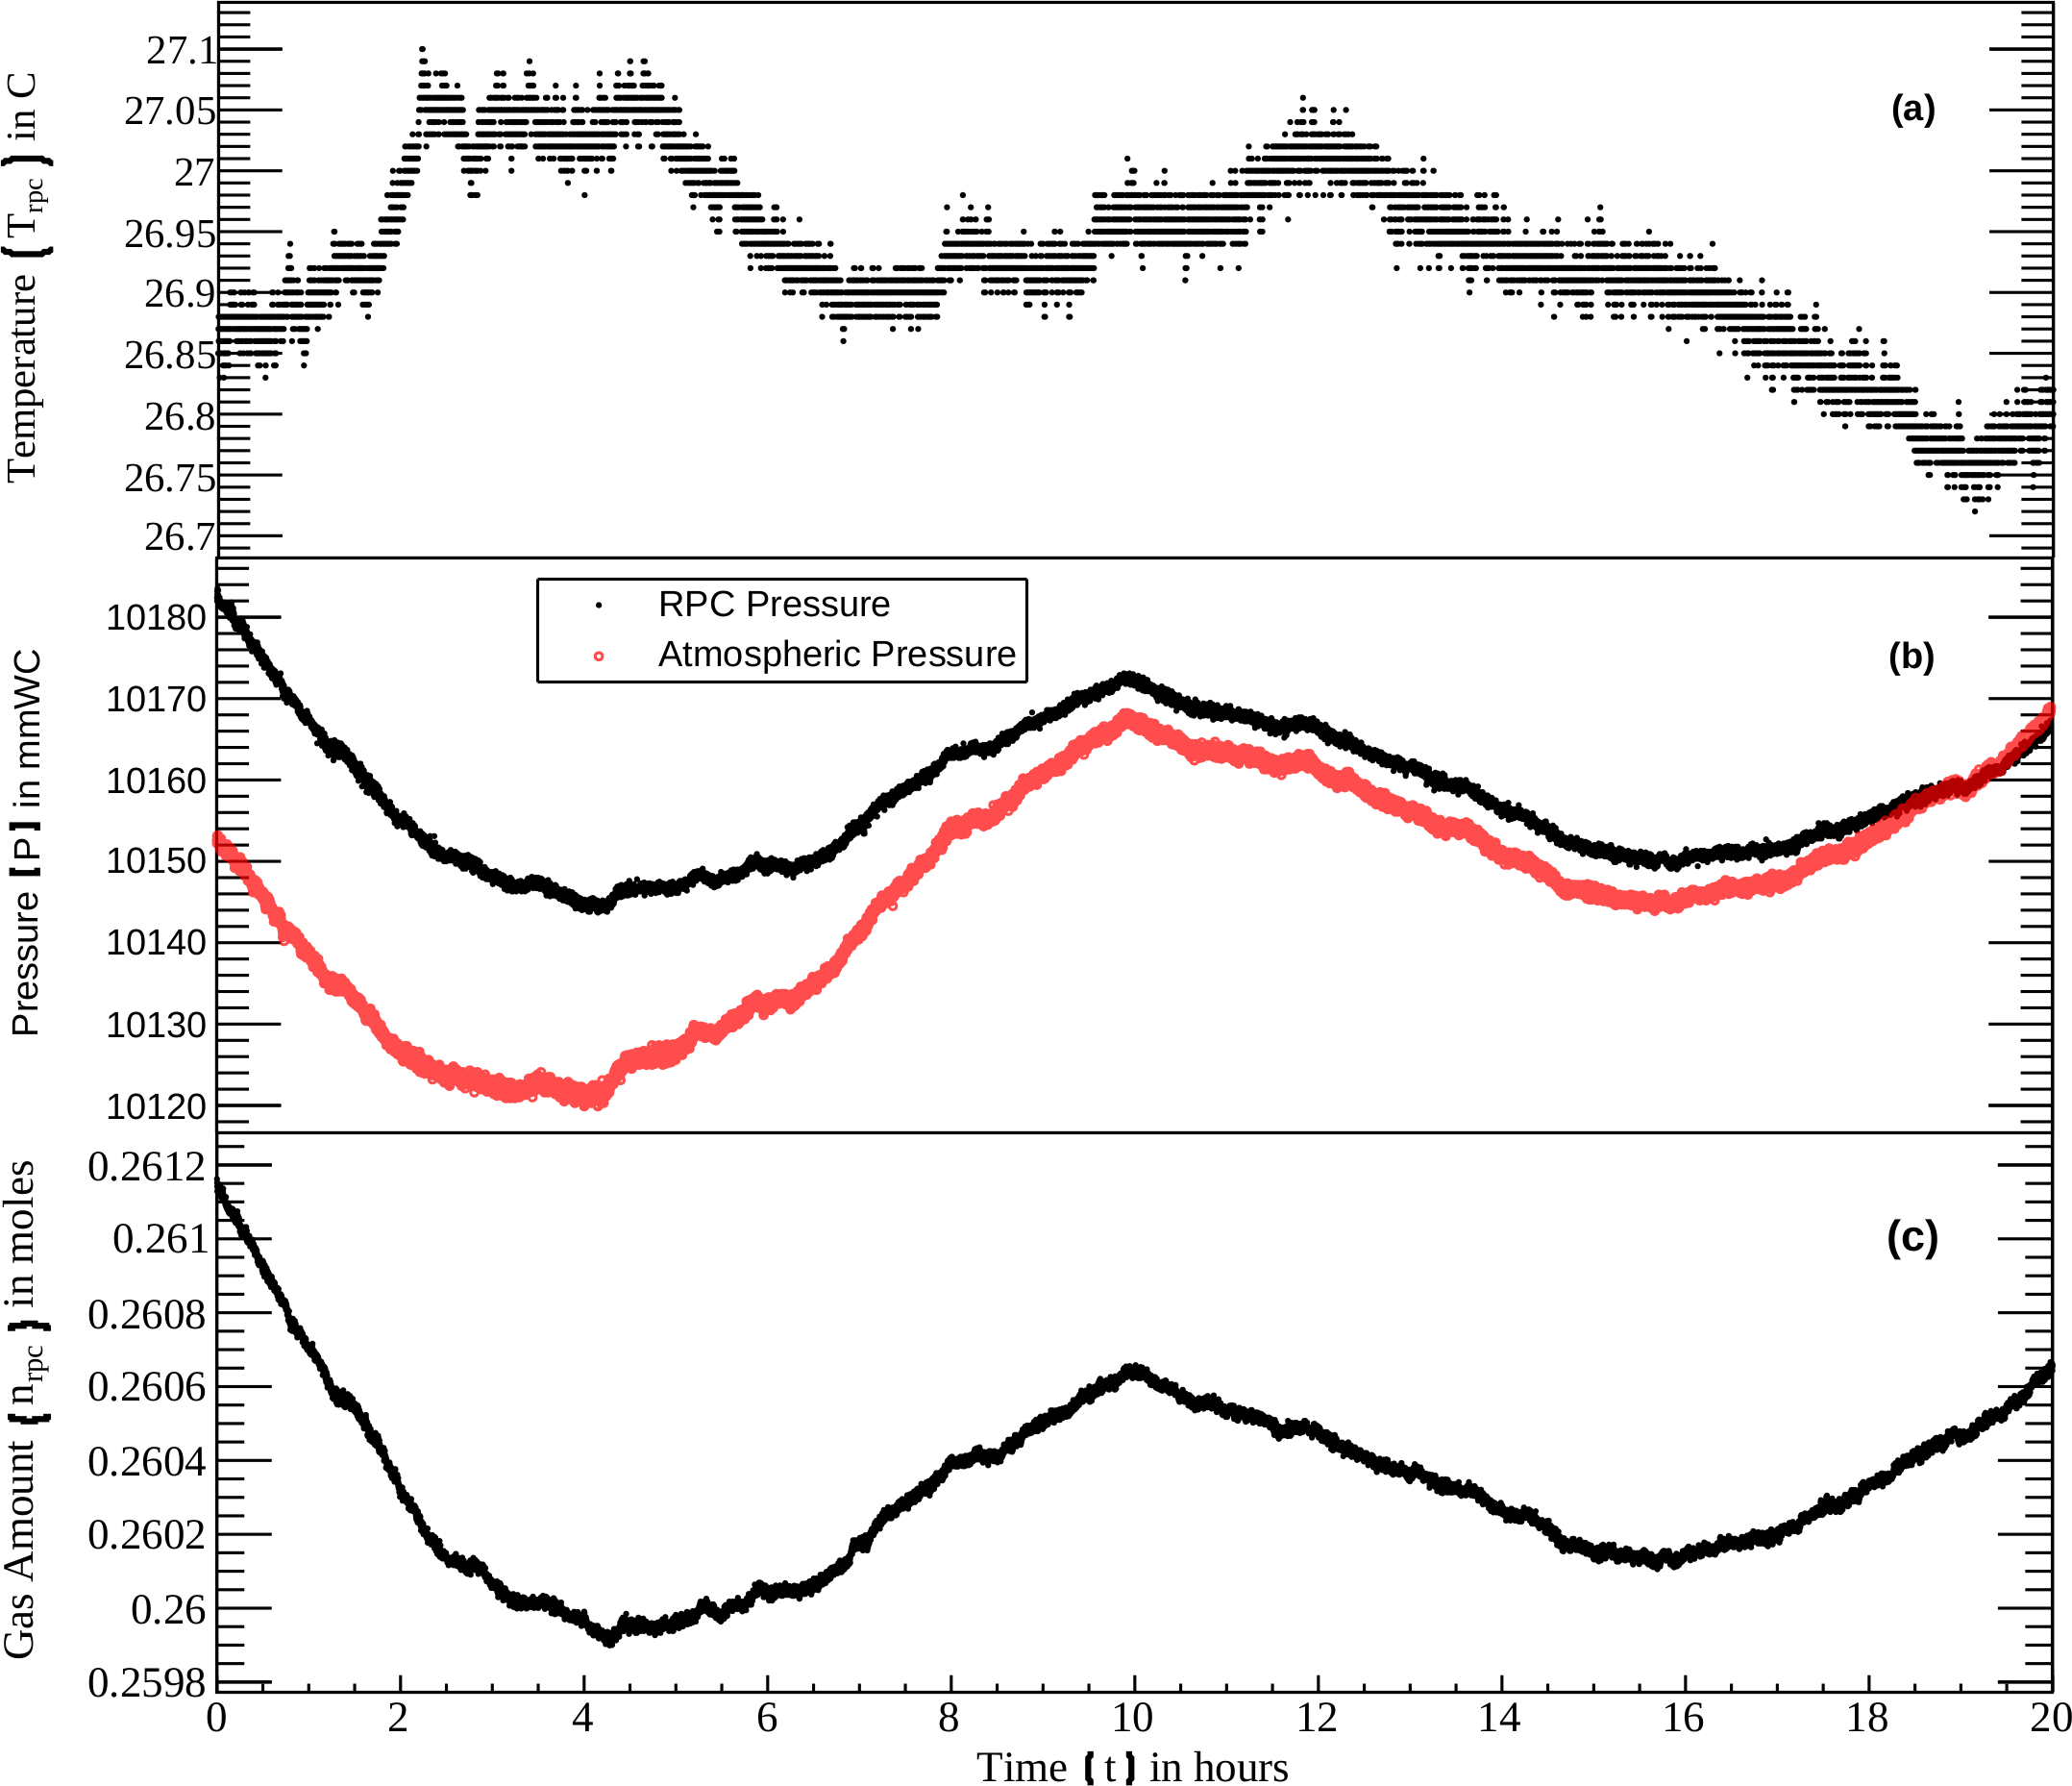
\includegraphics[width=0.7\textwidth]{all_57_gen.png}
    \vspace{-8pt}
    \caption{Gas amount was calculated using $n_{\text{rpc}}=\frac{P_{\text{rpc}}V_{\text{rpc}}}{RT_{\text{rpc}}}$ with $V_{\text{rpc}}=6.3$\,L}
  \end{figure}
\end{frame}

\begin{frame}
  \frametitle{Leak Test : Analysis}
  The volume of the gas gap changes due to the variations in the
  atmospheric pressure and the room temperature. To compensate for
  this change in volume, the volume of the RPC gap at time $t$ is
  represented by the following equation.
  \[V_{\textrm{rpc}|t} = V_{\textrm{rpc}}\left(1-x_T\left(T_{\textrm{rpc}|t}-T_{\textrm{rpc}|t=0}\right)\right)\left(1-x_P\left(P_{\textrm{atm}|t}-P_{\textrm{atm}|t=0}\right)\right)\]
  To minimise the correction terms, $x_T$ and $x_P$, Poiseuille's
  equation was used.
  \[\left(\text{Flow Rate}\right)=\left(\text{Leak Constant}\right)\times\left(\text{Effective Pressure Difference}\right)\]
  \[\implies\left.\frac{\mathrm{d}n_{\textrm{rpc}}}{\mathrm{d}t}\right| _t=\textrm{C}_{\textrm{Leak}}\times\left(\frac {P_{{\textrm{rpc}|t} }^{2}-P_{{\textrm{atm}|t} }^{2}}{2P_{{\textrm{rpc}|t} }}\right)\]
\end{frame}

\begin{frame}
  \frametitle{Leak Test : Analysis}
  \begin{itemize}
  \item For different values of $x_T$ and $x_P$, Leak Rate $\left(\frac{\mathrm{d}n_{\textrm{rpc}}}{\mathrm{d}t}\right)$ is calculated for different point of time.
  \item The plot of $\frac{\mathrm{d}n_{\textrm{rpc}}}{\mathrm{d}t}$ vs $\frac{P_{\textrm{rpc}}^{2}-P_{\textrm{atm}}^{2}}{2P_{\textrm{rpc}}}$ is then fitted with a straight line and $\chi^2/\textrm{ndf}$ is calculated for each combination of $x_T$ and $x_P$.
  \item Particular combination of $x_T$ and $x_P$ will make $\chi^2/\textrm{ndf}$ minimum.
  \end{itemize}
  \begin{figure}[!h]
    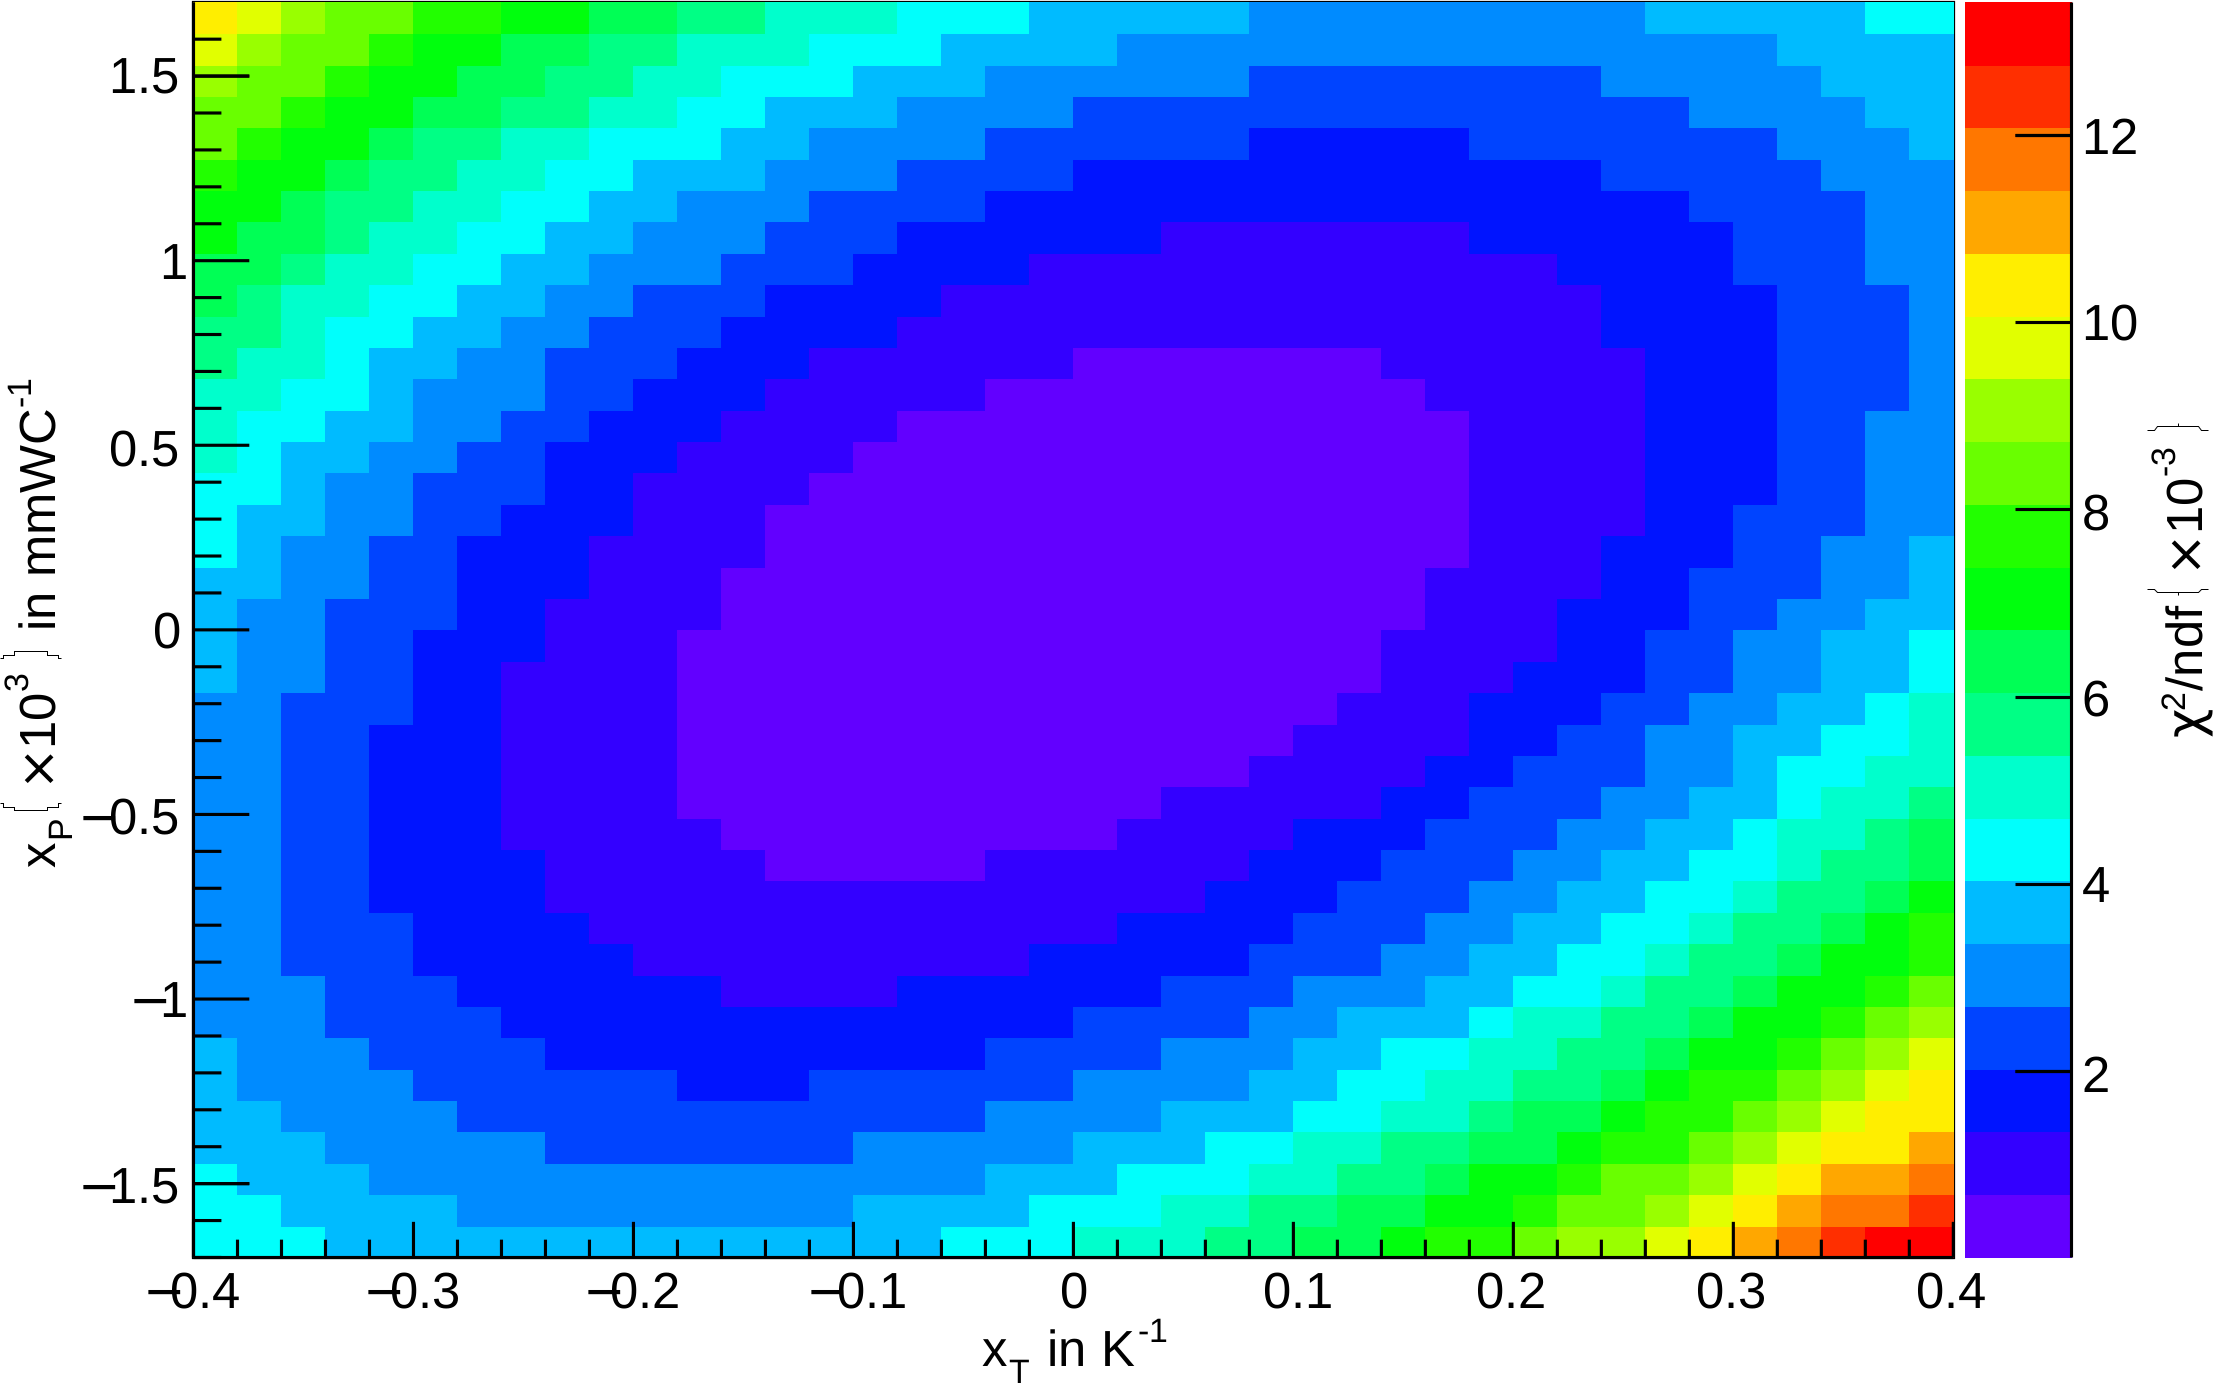
\includegraphics[width=0.65\textwidth]{cor_factors.png}
  \end{figure}
\end{frame}

\begin{frame}
  \frametitle{Leak Test : Analysis}
  \begin{figure}[!h]
    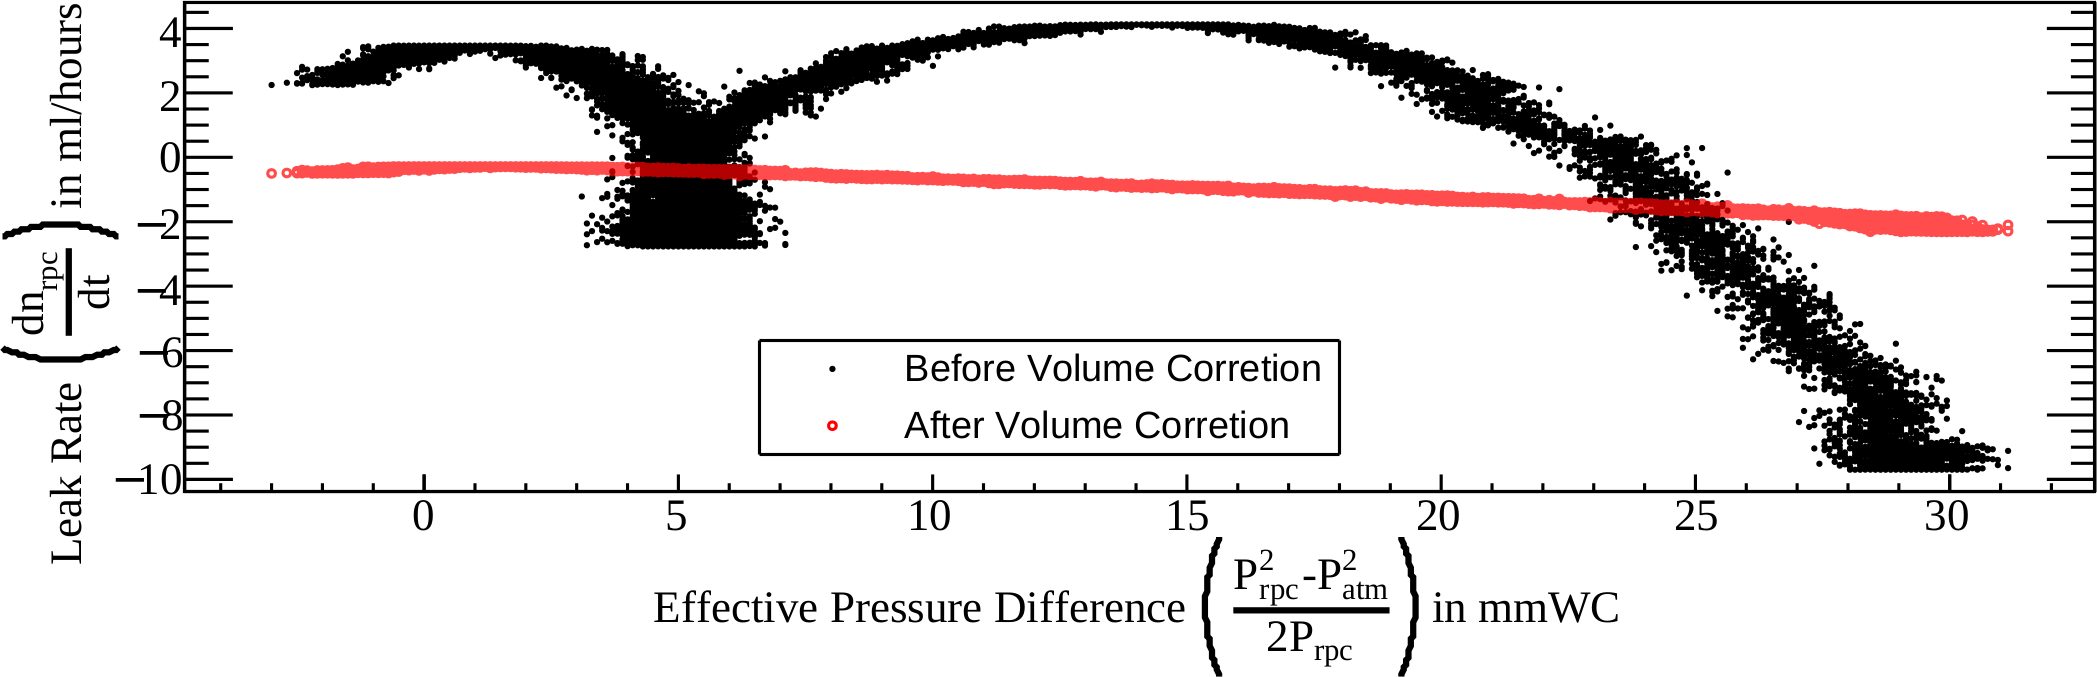
\includegraphics[width=0.85\textwidth]{Q_dP_57.png}
  \end{figure}
  \[\textrm{C}_{\textrm{Leak}}=-\left(6.73\pm 0.007\left(\textrm{stat}\right)\right)\times 10^{-2}\textrm{\,ml\,hour$^{-1}$\,mmWC$^{-1}$}.\]
  \begin{figure}[!h]
    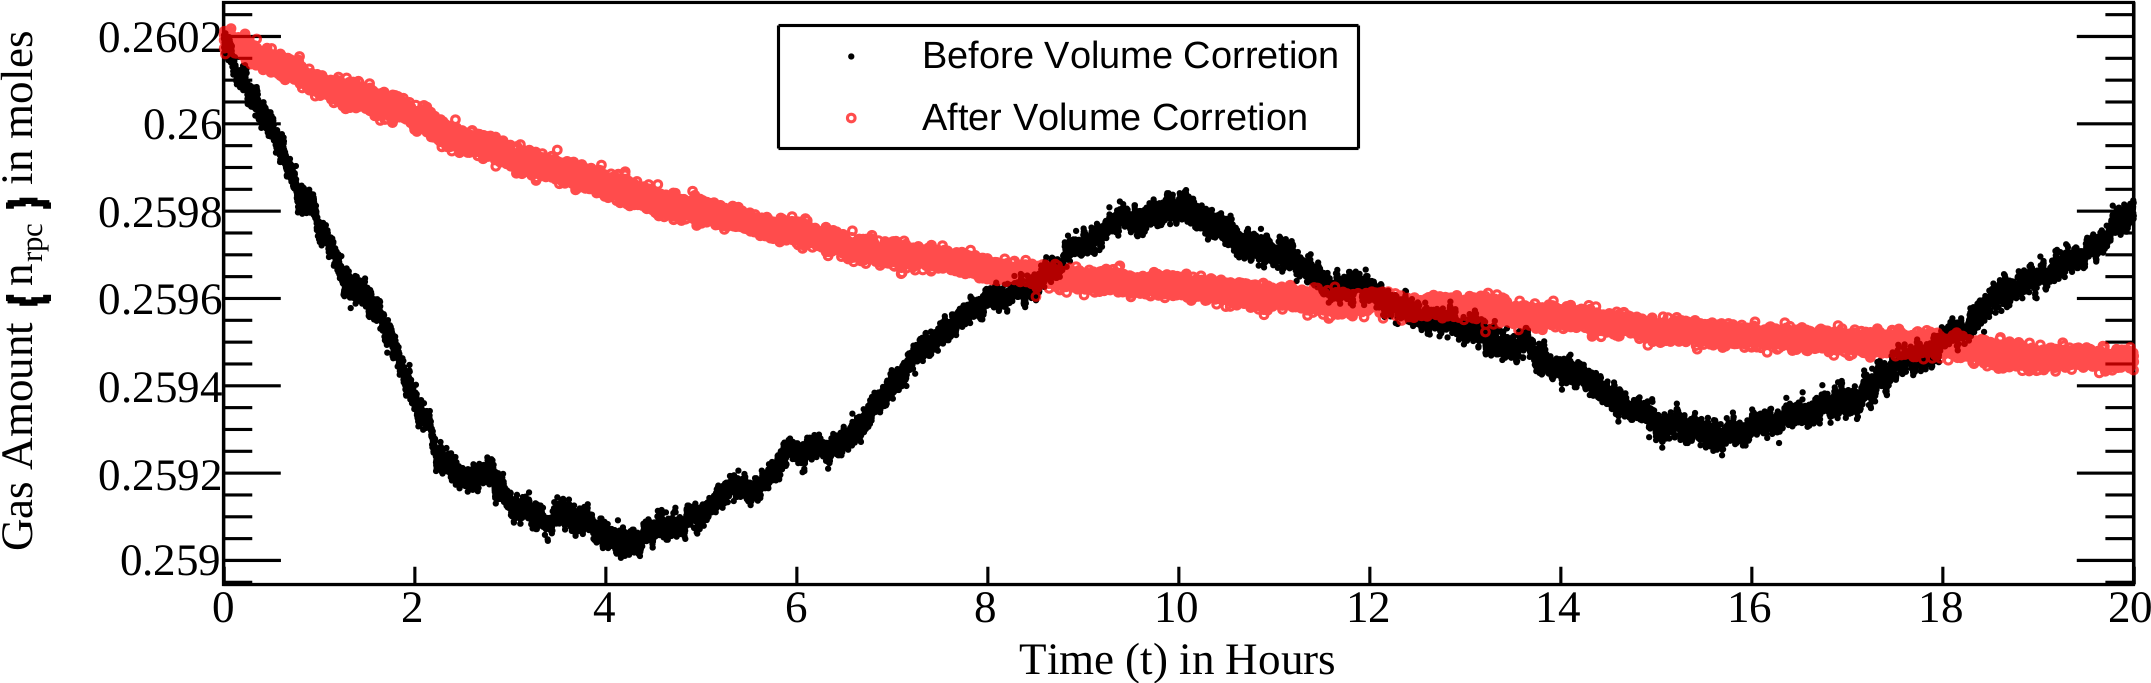
\includegraphics[width=0.85\textwidth]{M_t_57.png}
  \end{figure}
\end{frame}

\begin{frame}
  \frametitle{Leak Test : Gap-2}
  \begin{figure}[!h]
    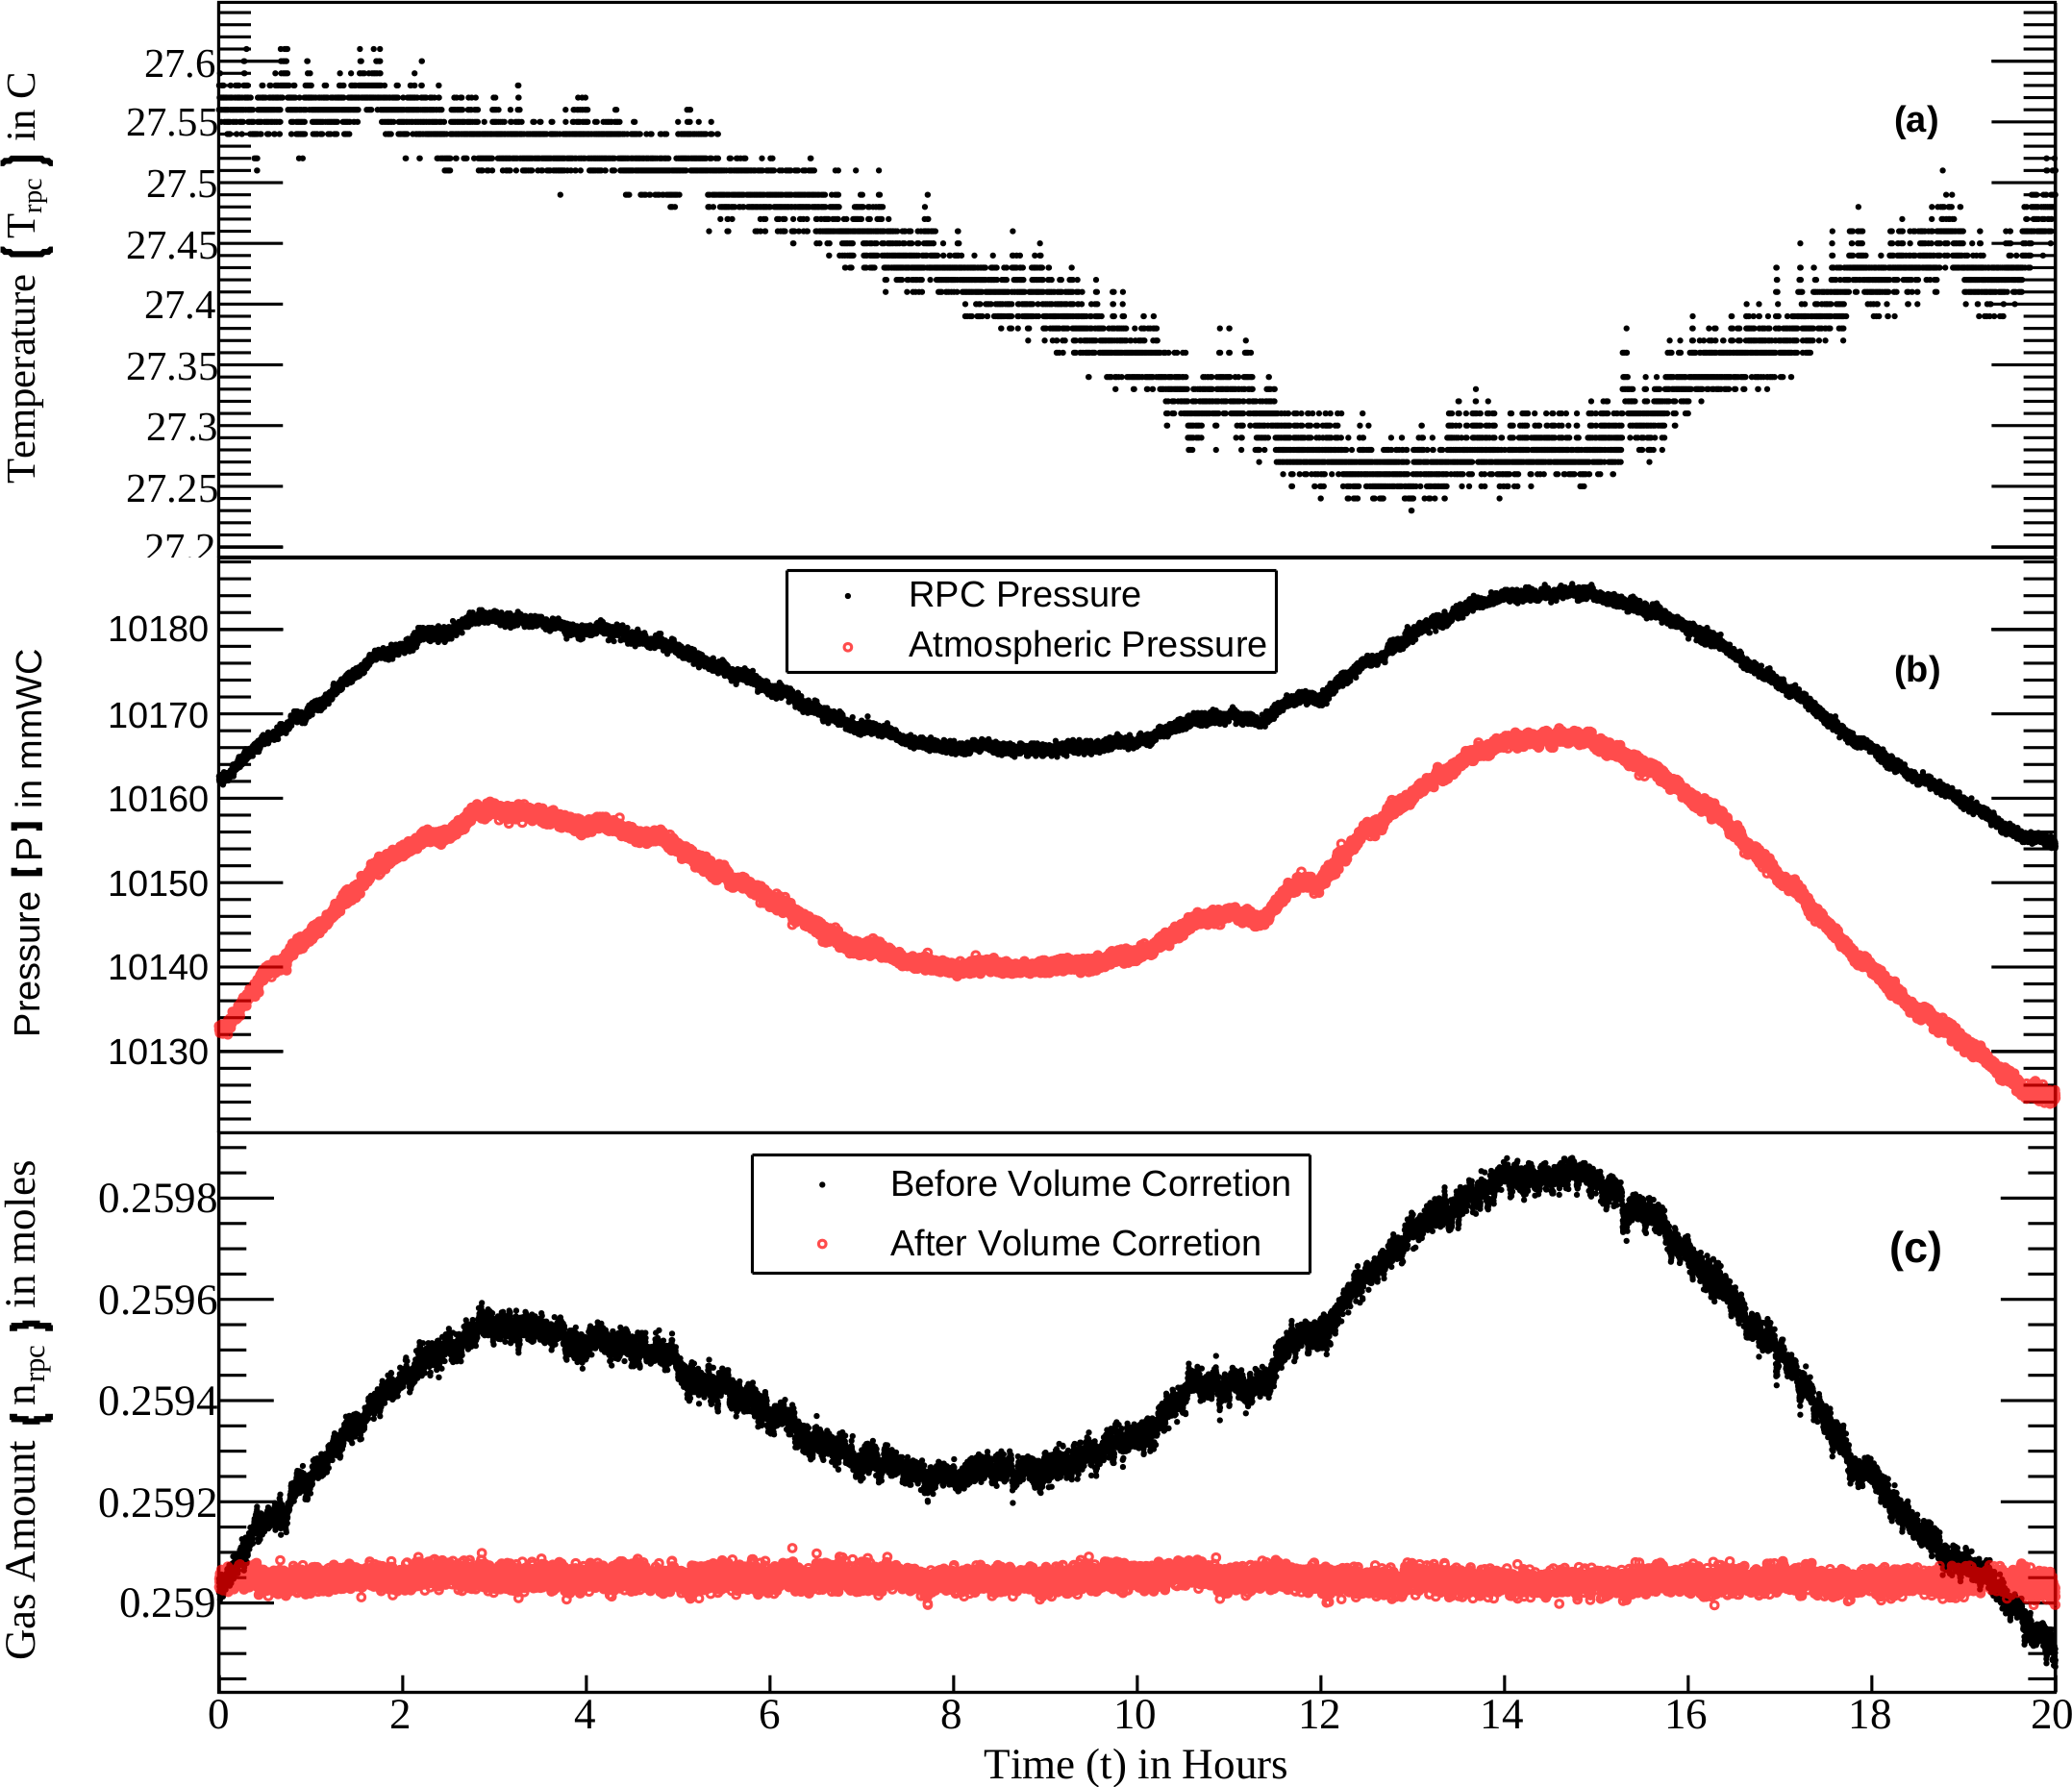
\includegraphics[width=0.7\textwidth]{all_130_gen.png}
    \vspace{-8pt}
  \end{figure}
  \[\textrm{C}_{\textrm{Leak}}=-\left(5.1\pm 0.15\left(\textrm{stat}\right)\right)\times 10^{-4}\textrm{\,ml\,hour$^{-1}$\,mmWC$^{-1}$}.\]
\end{frame}

%GMA Add figure 2.14 from your thesis in next page
%GMA Also mention the threshold value for acceptance

\begin{frame}
  \frametitle{Leak Test : Threshold}
  \begin{figure}[!h]
    \vspace{-8pt}
    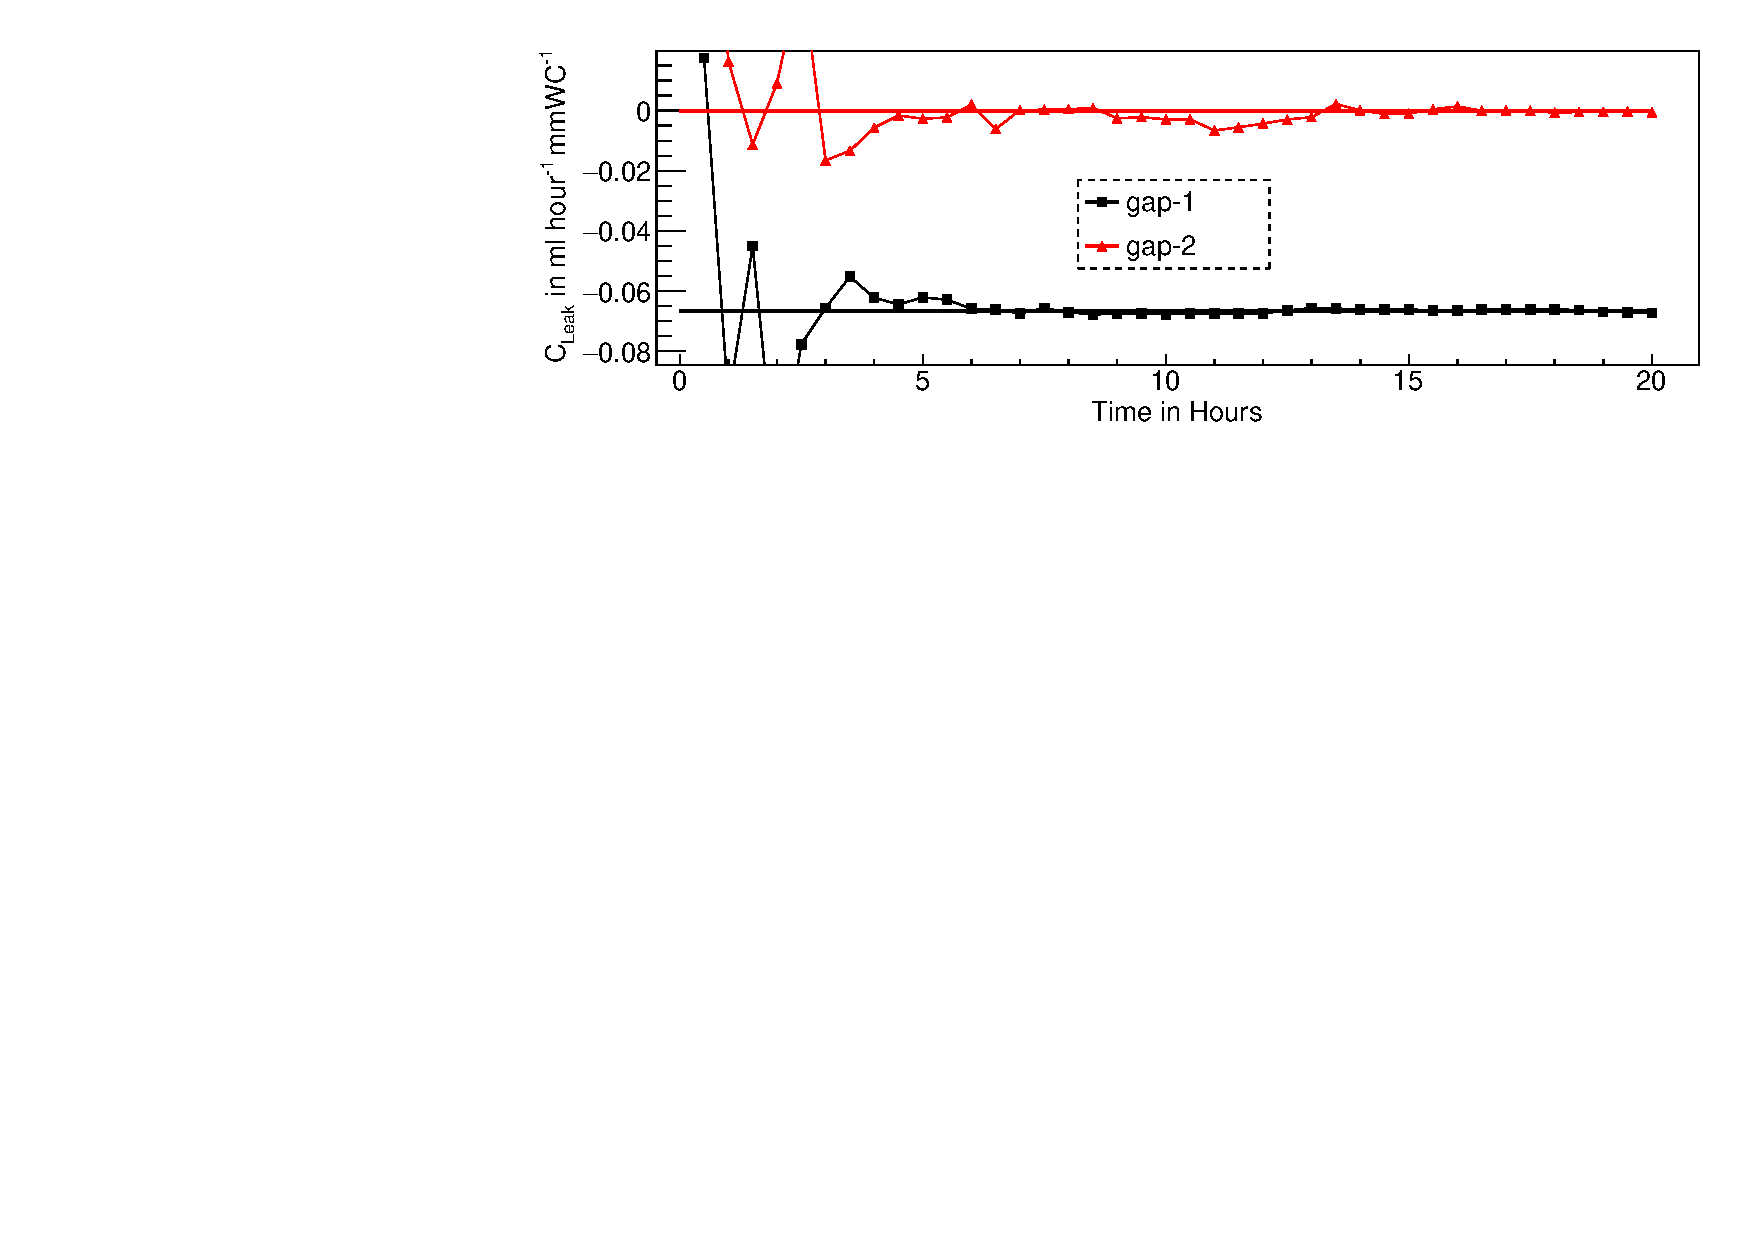
\includegraphics[width=0.99\textwidth]{conf_57_130.pdf}
    \vspace{-8pt}
  \end{figure}
  \begin{itemize}
  \item A smaller leak requires longer time to estimate.
  \item Most of the cases, a minimum of 7-8 hours is required to
    estimate the leakage without significant uncertainty.
  \item Currently, a gas gap is considered as usable if its
    $\textrm{C}_{\textrm{Leak}}$ value is greater than
    $-0.02$\,ml\,hour$^{-1}$\,mmWC$^{-1}$.
  \end{itemize}
\end{frame}

\begin{frame}
  \frametitle{Leak Test : Error}
  Multiple data samples are extracted from a large data sample of
  48\,hours and `$\textrm{C}_{\textrm{Leak}}$'s are calculated for each
  of them. The standard deviation of these estimated
  `$\textrm{C}_{\textrm{Leak}}$'s, is calculated and treated as the
  systematic error. 
  \begin{figure}[!h]
    \vspace{-8pt}
    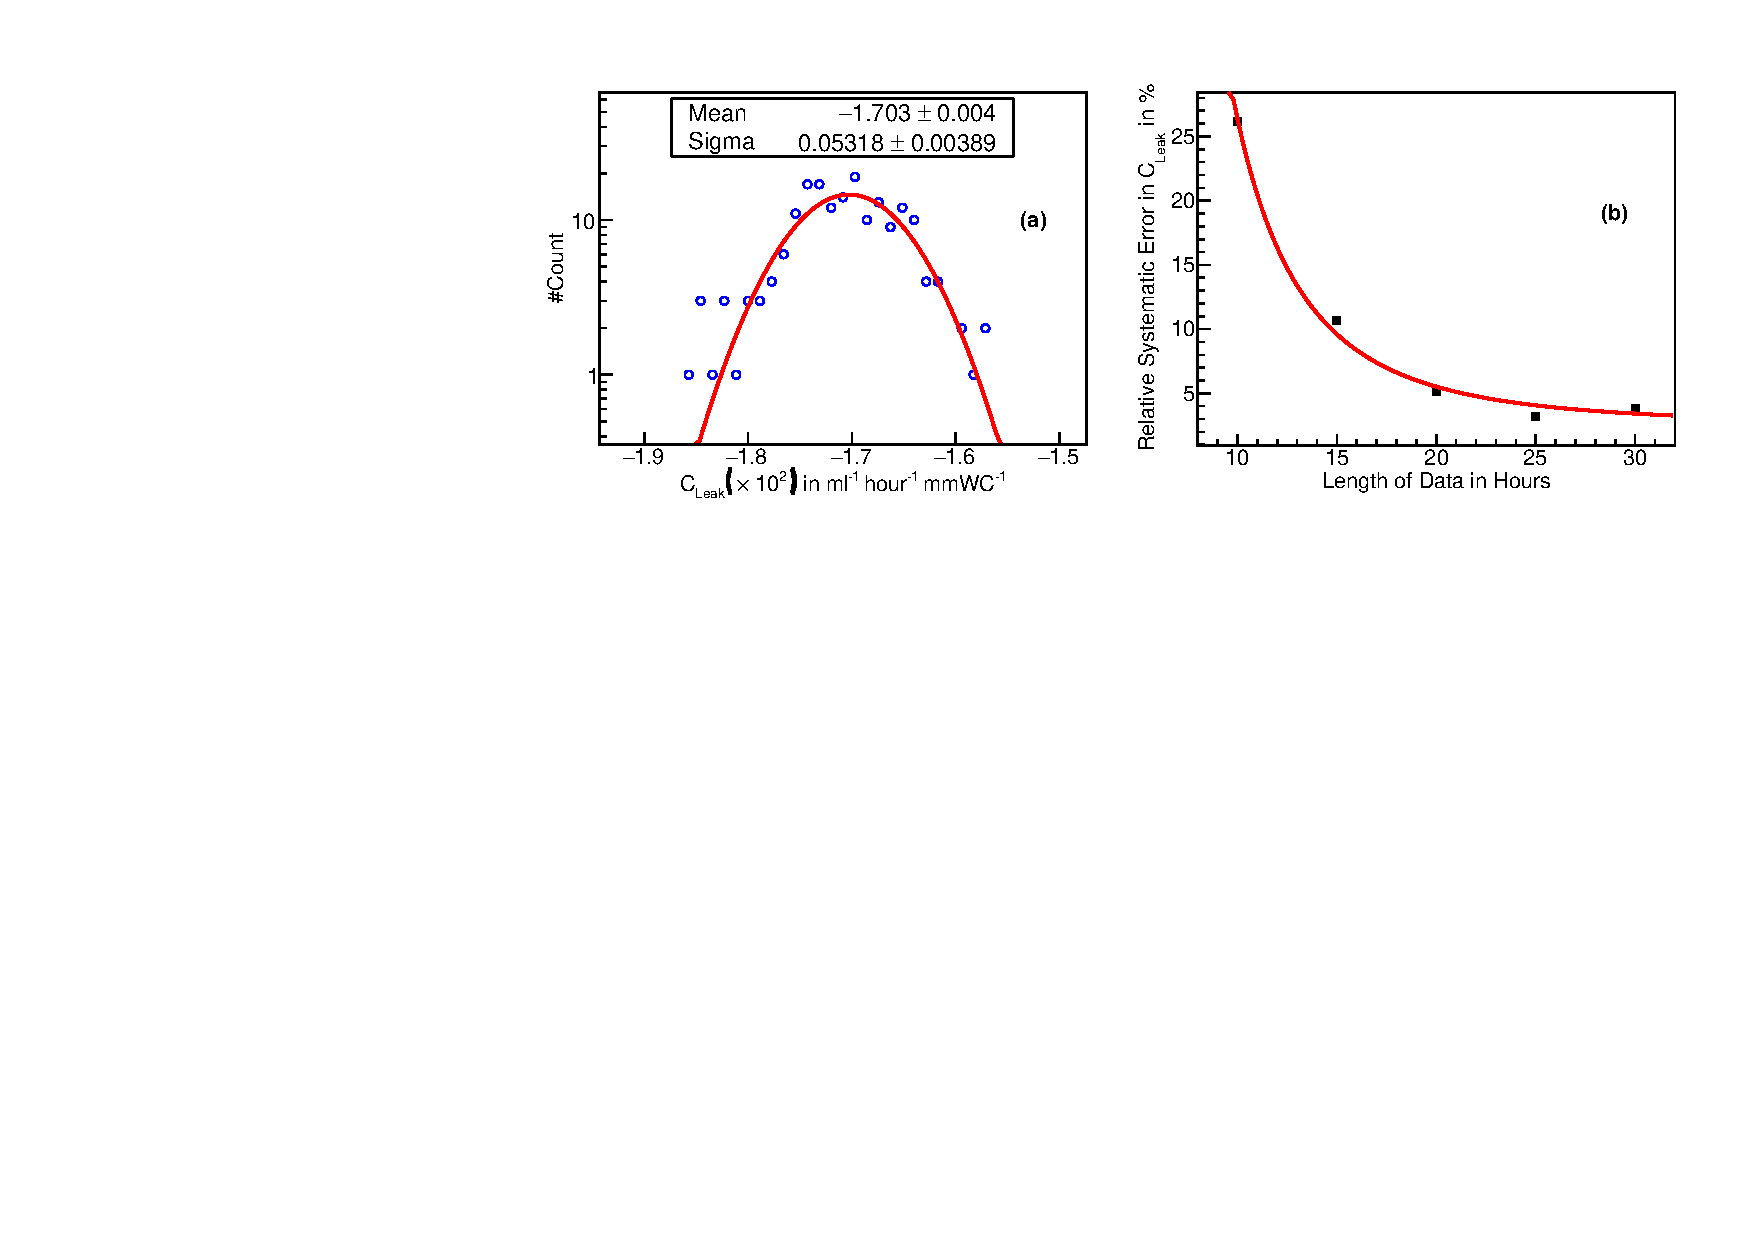
\includegraphics[width=0.99\textwidth]{splitDataLeak.pdf}
    \vspace{-8pt}
  \end{figure}
  \vspace{20pt}
  \href{https://doi.org/10.1088/1748-0221/14/04/P04009}{DOI:10.1088/1748-0221/14/04/P04009} \hspace{10pt} \href{https://arxiv.org/abs/1812.00277}{arXiv:1812.00277}
  %% \url{DOI:10.1088/1748-0221/14/04/P04009} \url{arXiv:1812.00277}
\end{frame}


%% Multiple Track Part

\begin{frame}
  \frametitle{Cosmic Ray Charged-particle multiplicity at Madurai}
  \begin{itemize} %\itemsep -1pt
  \item The principal aim of this work is to observe the charged-particle multiplicity in the atmospheric muon data collected at IICHEP Madurai and compare it with the air shower simulation.
  \item Multiple tracks can be detected in the detector when more than one particles pass through within the same trigger window.
  \item Multiple tracks can occur due to muons or other particles.
  \item The sources of the particles may be one or multiple cosmic ray showers.
  \end{itemize}
\end{frame}

\begin{frame}
  \frametitle{Detector Setup : 12 Layers of 2\,m$\times$2\,m RPCs}
  \begin{figure}[h]
    \centering
    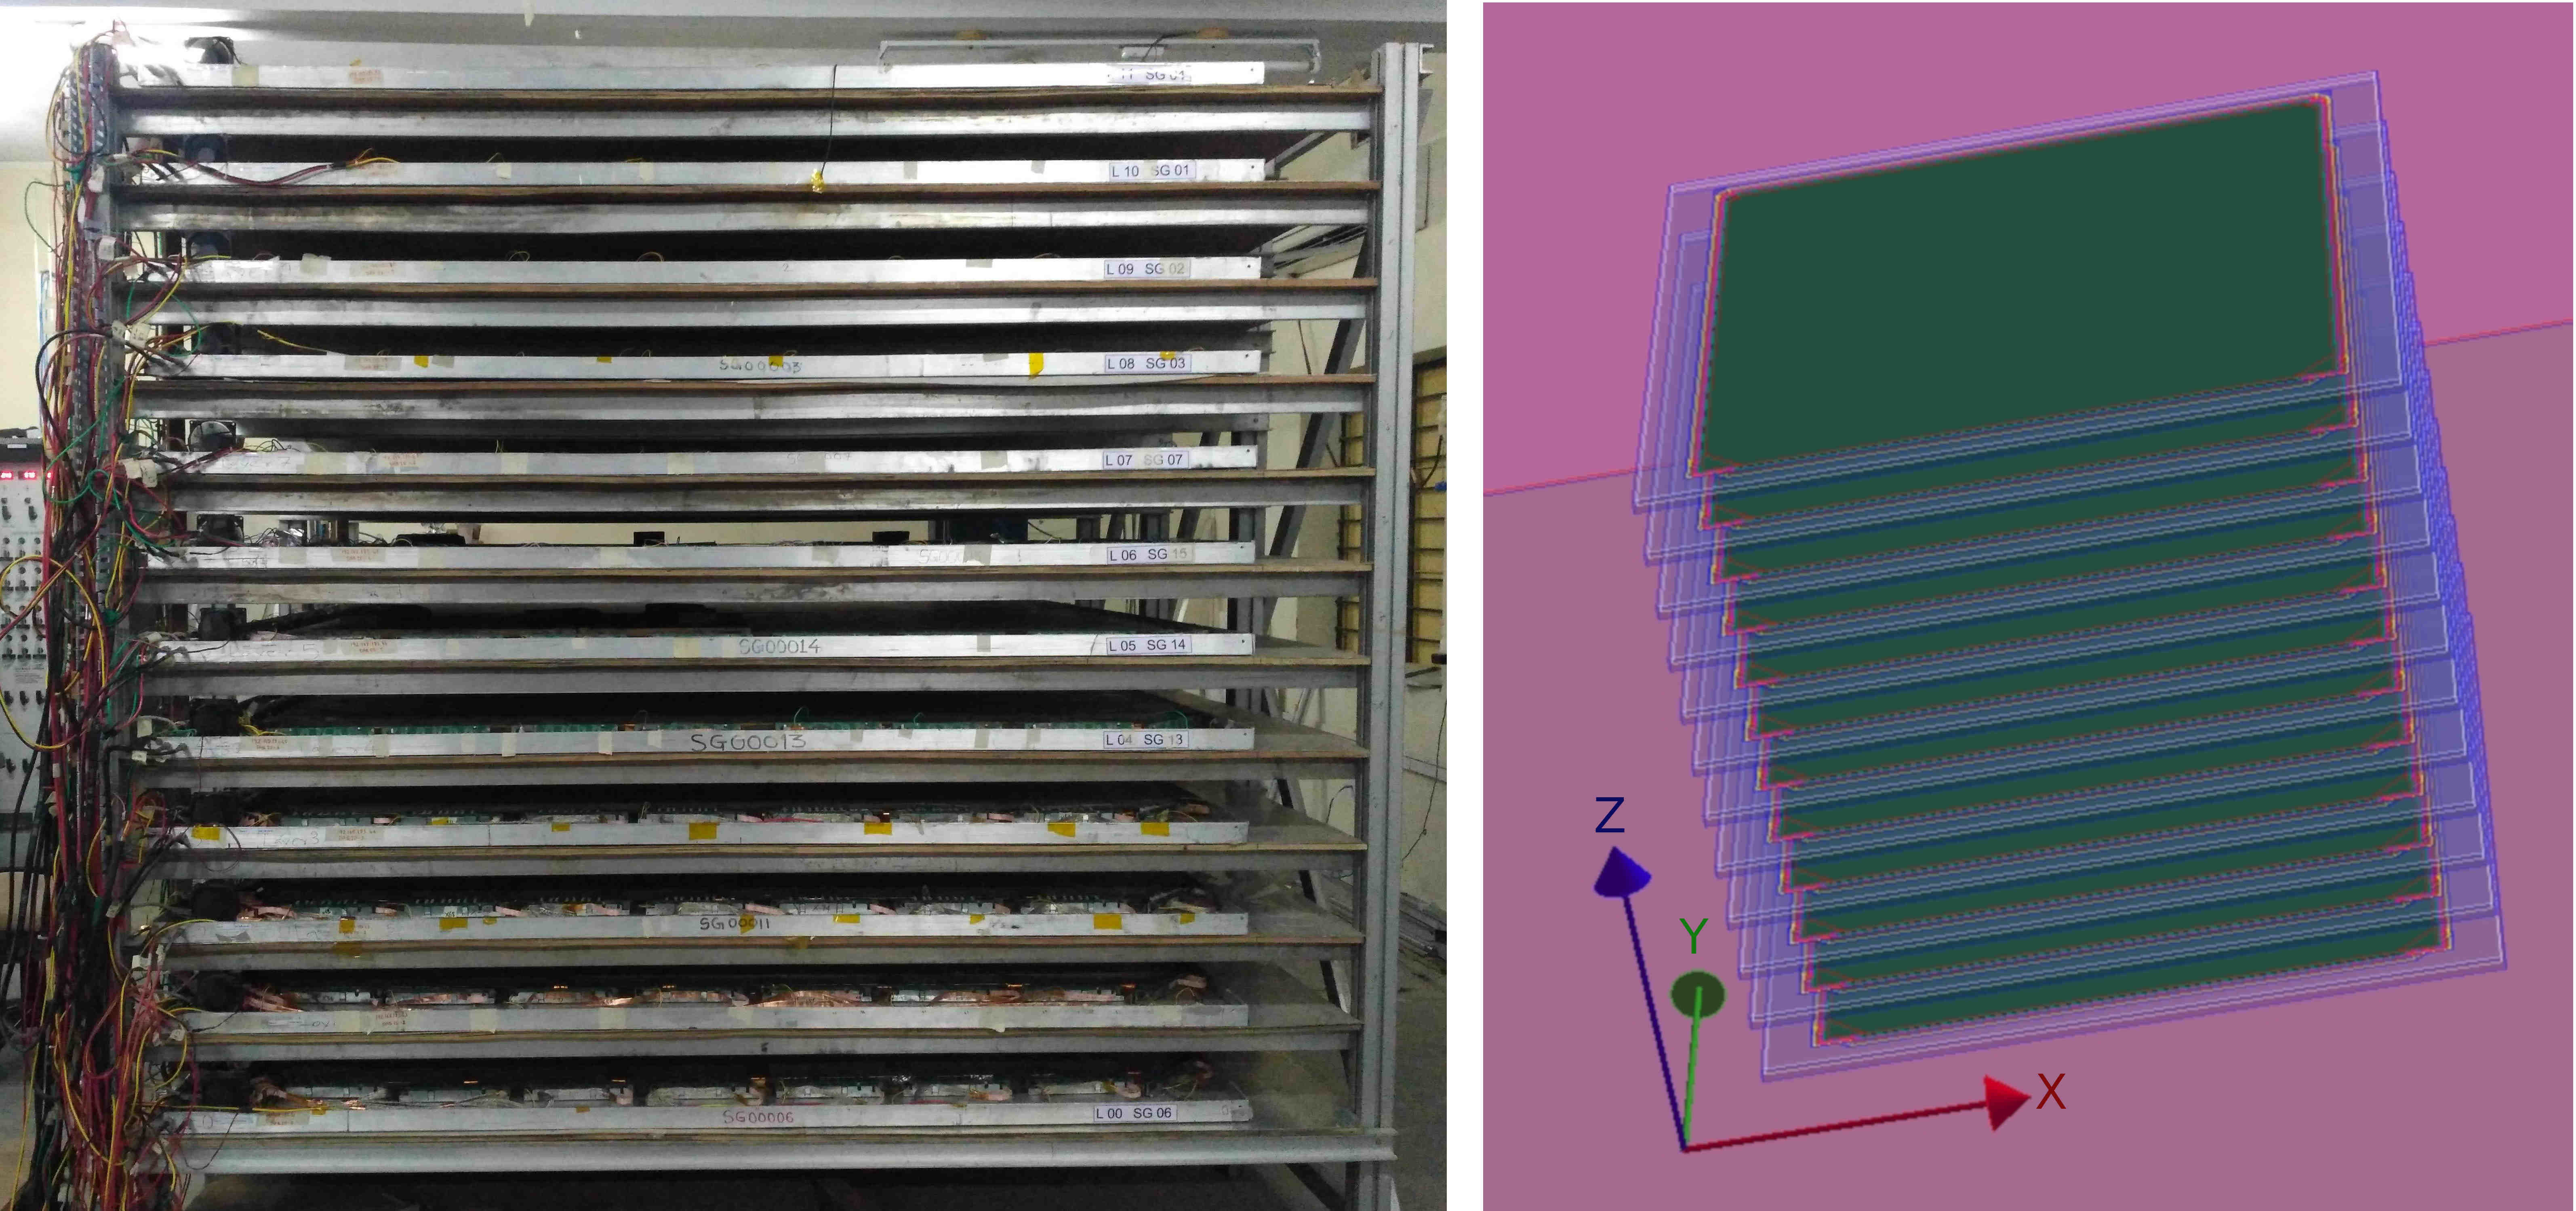
\includegraphics[width=0.99\linewidth]{ABlockStackiDAQ_new.jpg} 
  \end{figure}
\end{frame}

\begin{frame}
  \frametitle{Multiple Tracks: Example}
  \begin{figure}[!h]
    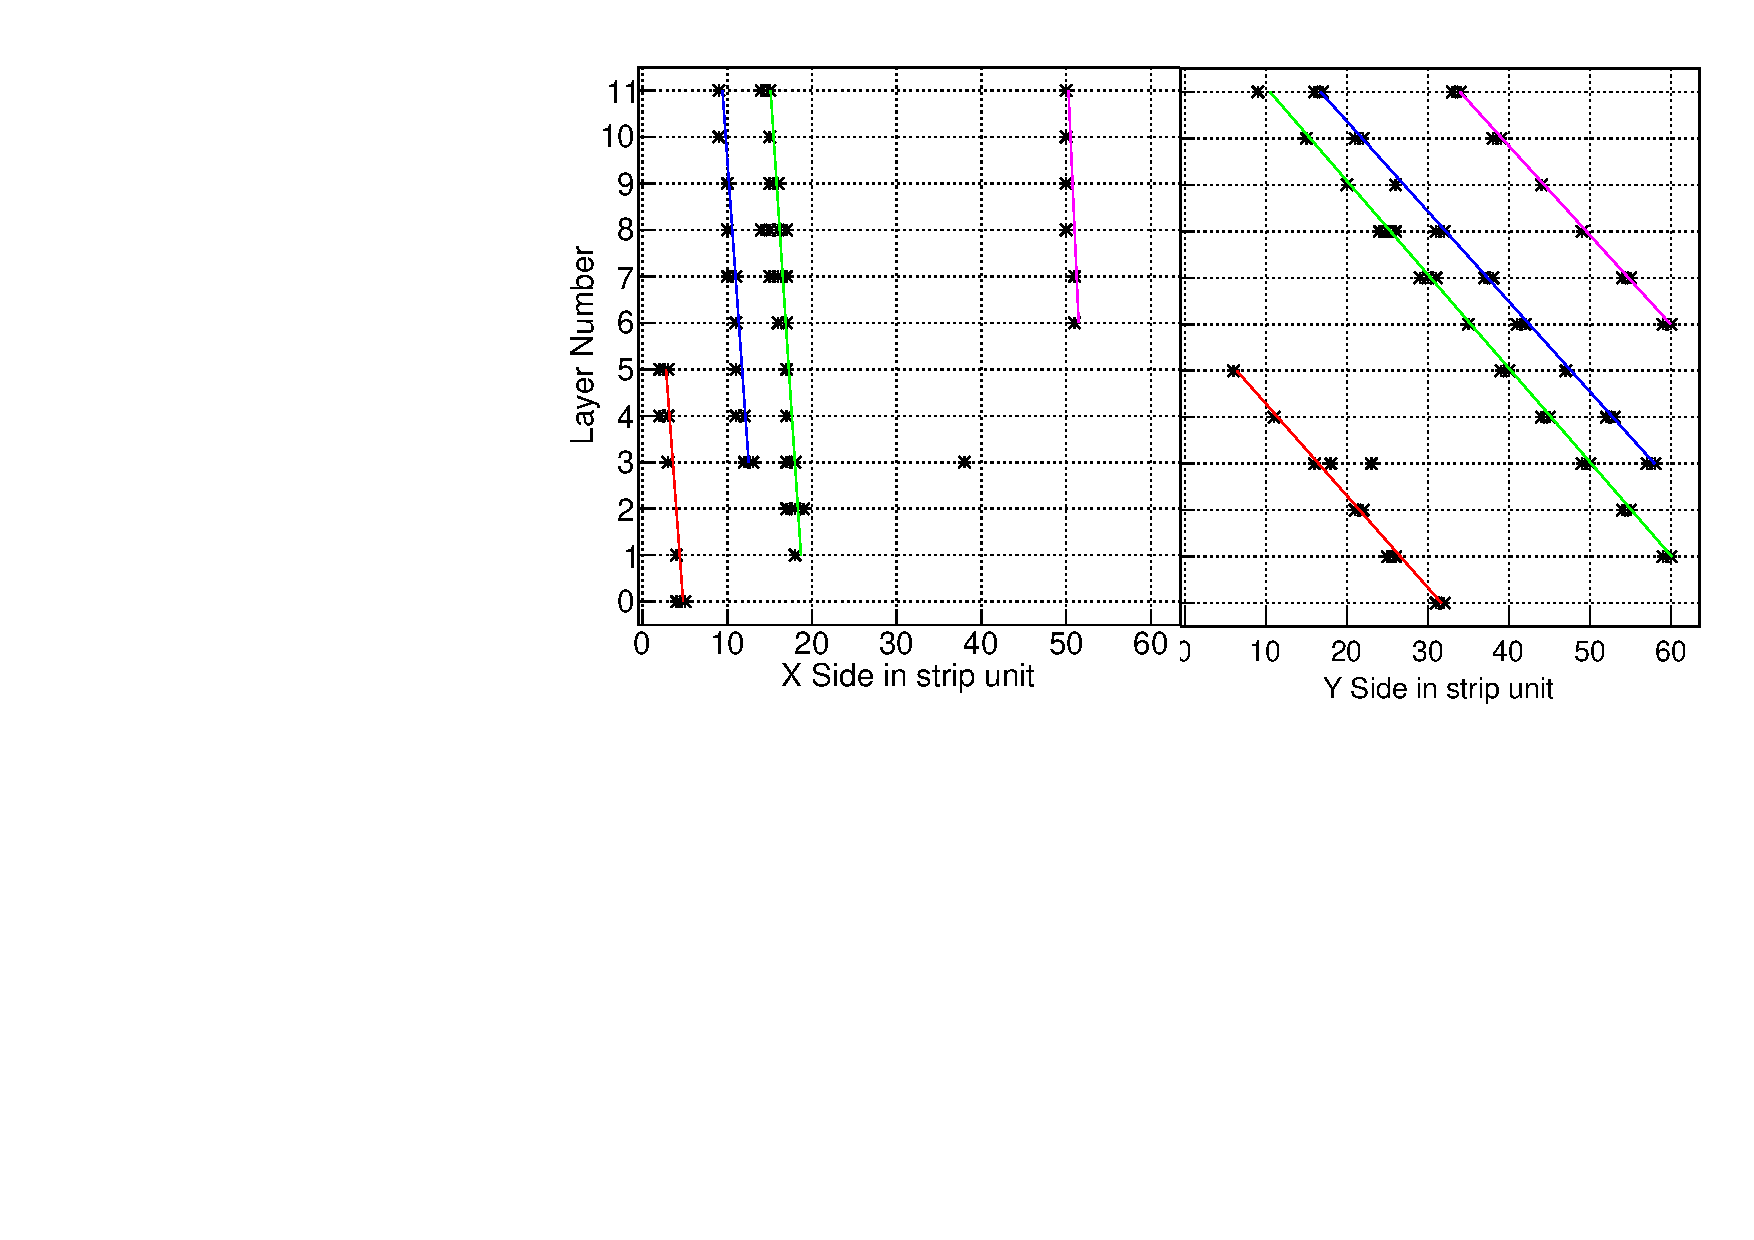
\includegraphics[width=0.99\textwidth]{Multi_Event_20170831_021424_386176_m4_1.pdf}
  \end{figure}
\end{frame}

\begin{frame}
  \frametitle{Multiple Tracks: Example}
  \begin{figure}[!h]
    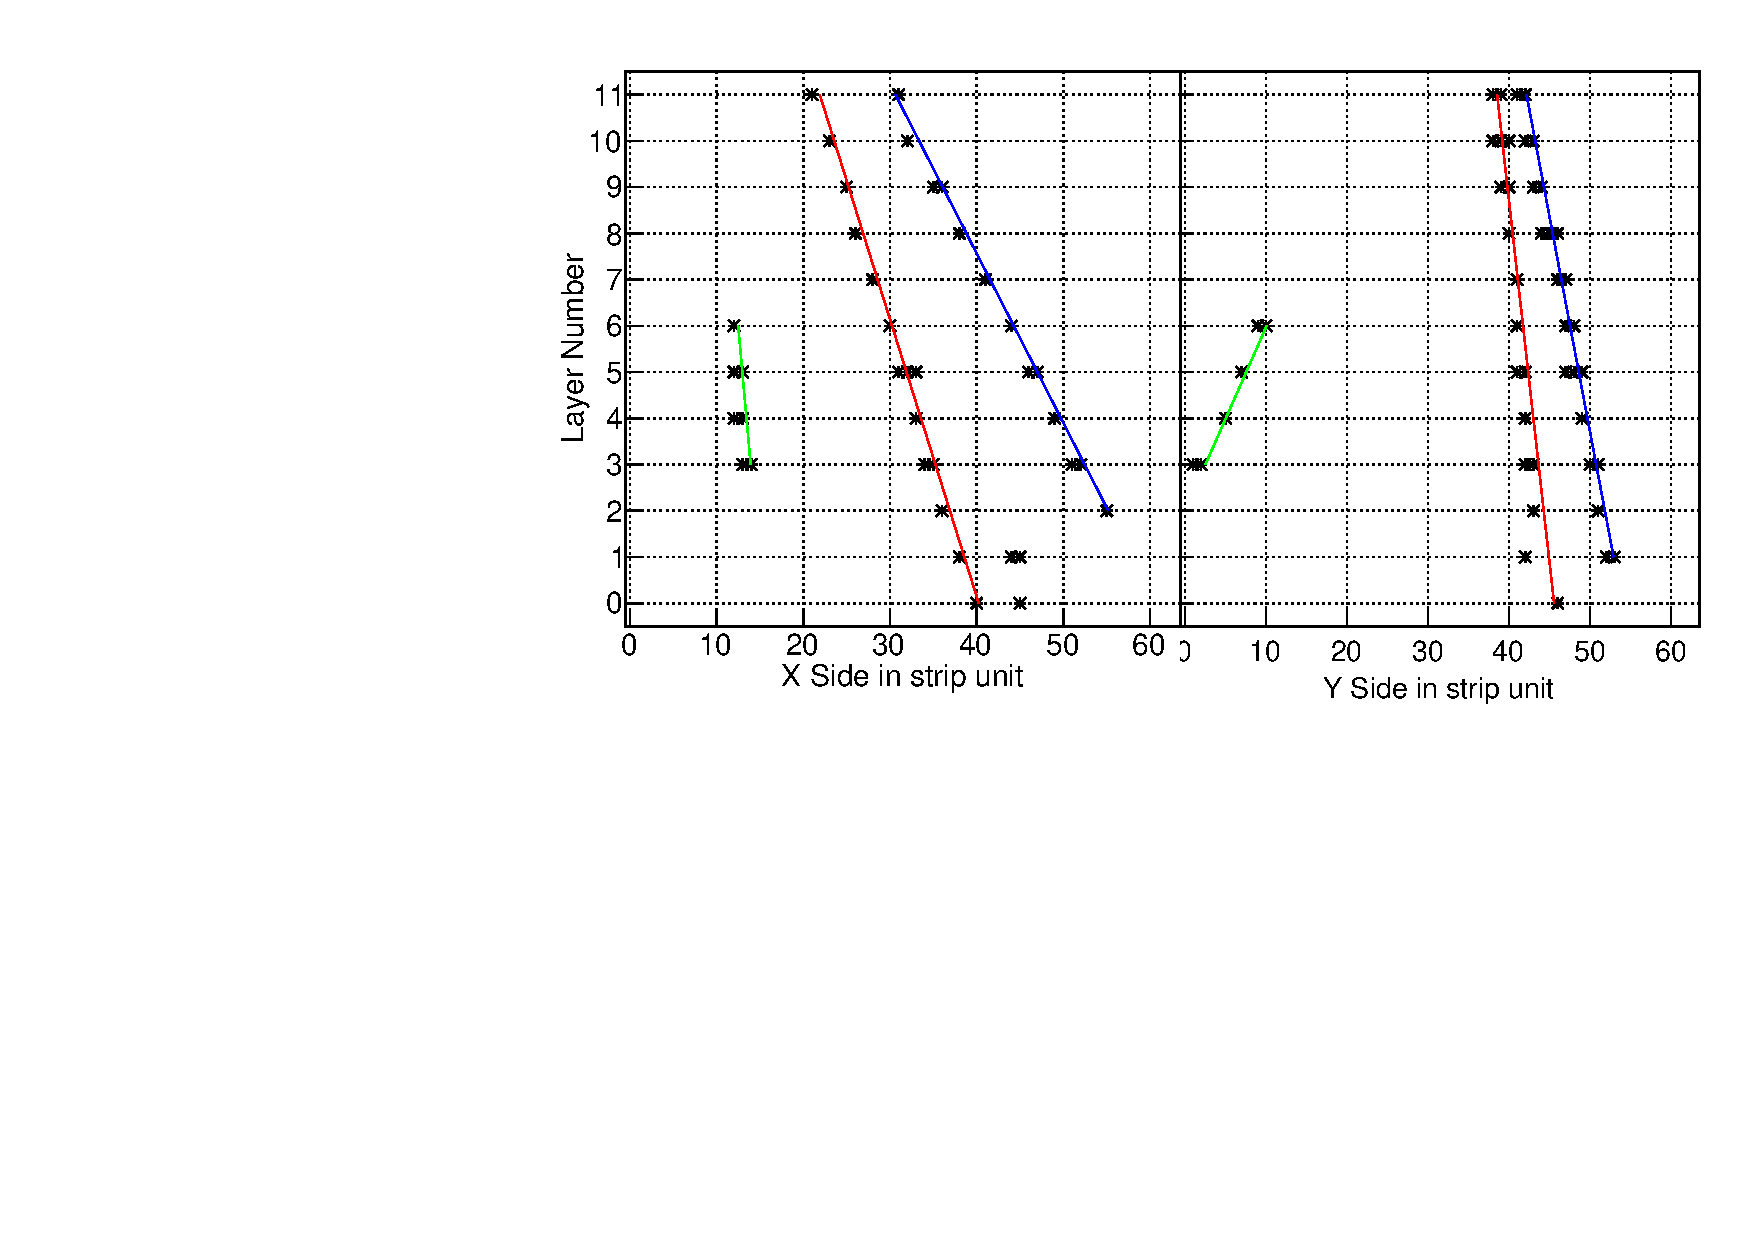
\includegraphics[width=0.99\textwidth]{Multi_Event_20170823_102605_9676_Roof_1.pdf}
  \end{figure}
\end{frame}


\begin{frame}
  \frametitle{Detector Simulation}
  \begin{itemize} %\itemsep -1pt
  \item Detector Simulation is performed using the GEANT4 toolkit
    (\url{QGSP_BERT_HP}).
  \item CORSIKA (\url{GHEISHA} \& \url{QGSJET}) generated secondaries
    are used as the input to the GEANT4 Simulation.
  \item Detector parameters (efficiency, noise and strip
    multiplicity) are incorporated in digitisation stage.
  \end{itemize}
  \begin{figure}[!h]
    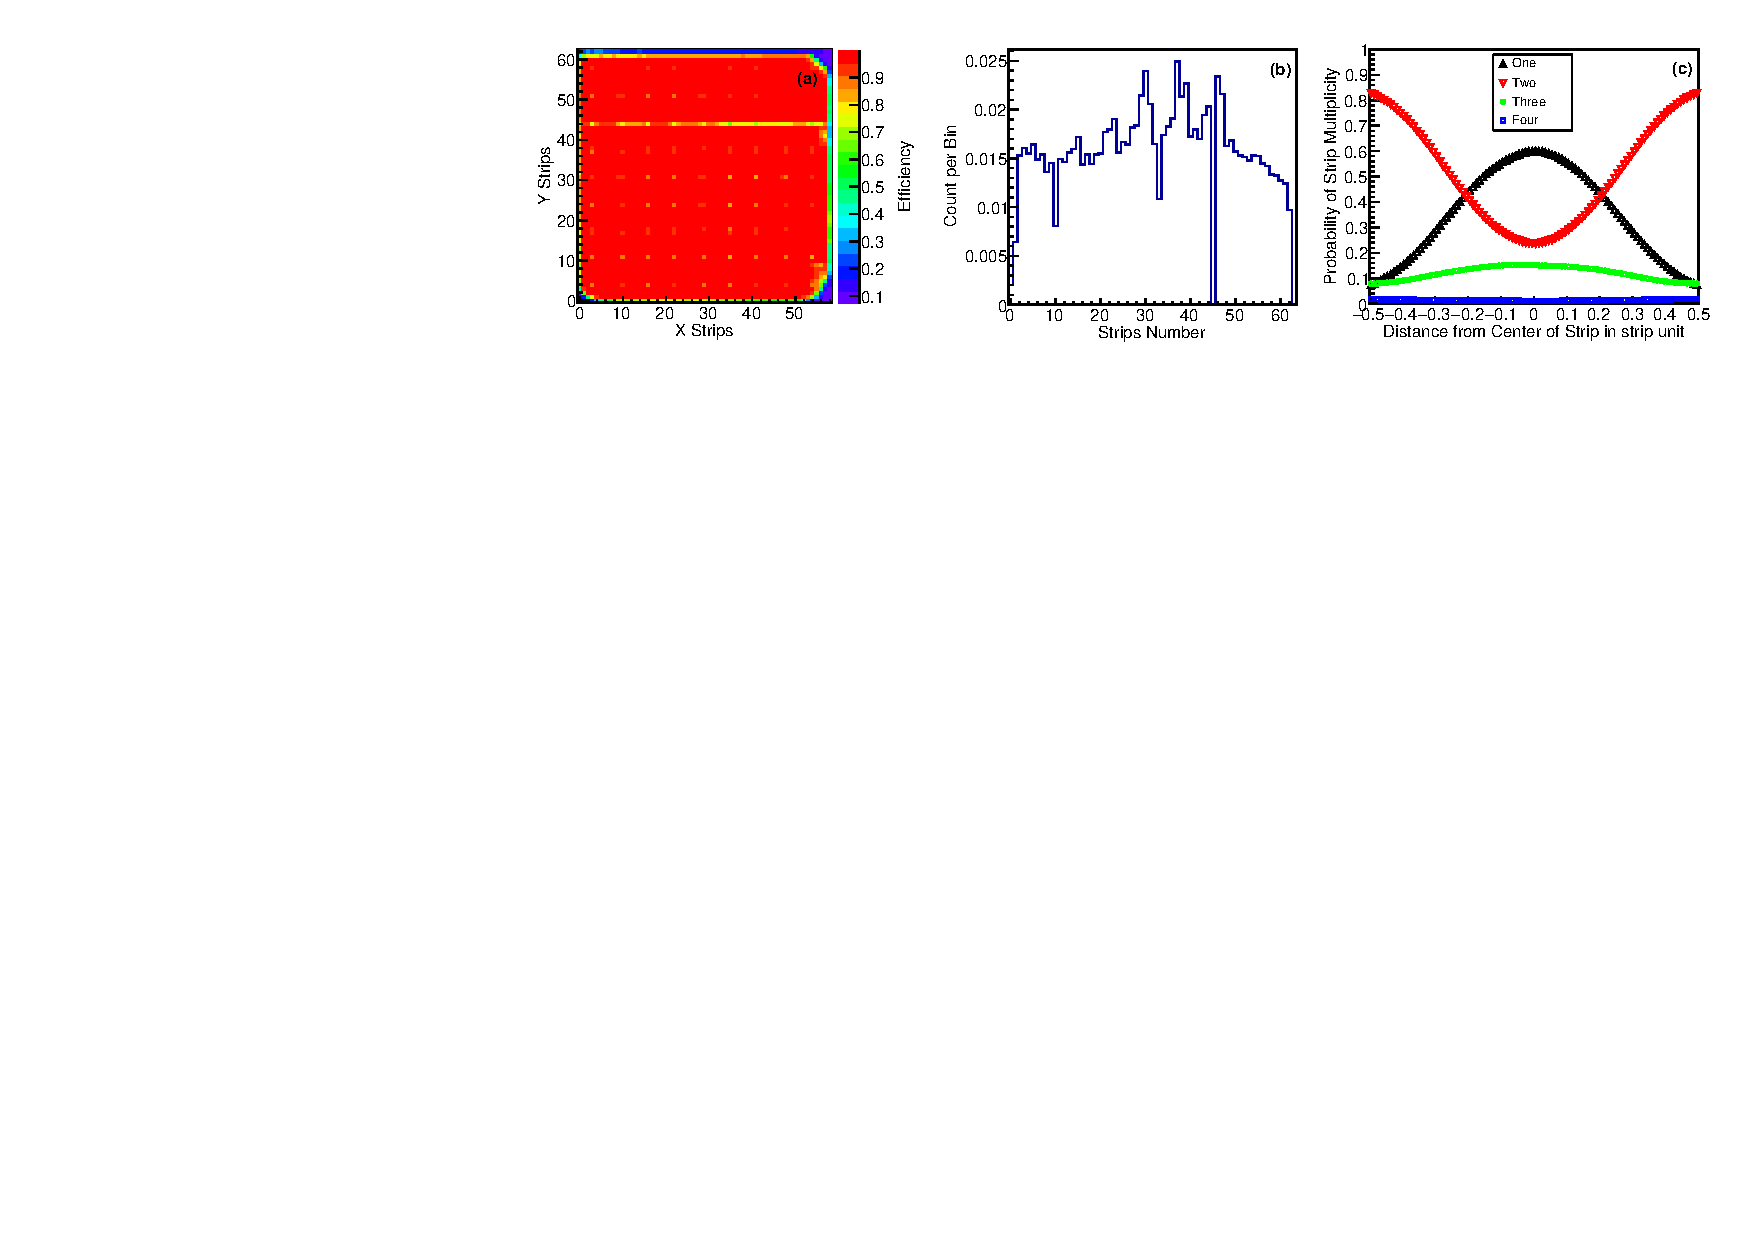
\includegraphics[width=0.99\textwidth]{layer2properties.pdf}
  \end{figure}
\end{frame}

\begin{frame}
  \frametitle{Multiple Tracks: Separating Tracks}
  \begin{itemize} %\itemsep -1pt
  \item Hough Transformation with equation of Straight Line
    $r=x\cos\theta+y\sin\theta$ is used to detect projections of track
    in Z-X \& Z-Y Planes.
  \item Showers and Noisy events rejected using various criteria.
  \item Projections on Z-X \& Z-Y Planes are combined using timing,
    track length and missing hits.
  \item Tracks generated inside the detector or in the roof of the
    building are rejected by calculating the skewed angle and the
    vertex position.
  \end{itemize}
  \begin{figure}[!h]
    \vspace{-6pt}
    \includegraphics[width=0.8\textwidth]{hough_plane_new.pdf}
  \end{figure}
\end{frame}

\begin{frame}
  \frametitle{Multiple Tracks: Rejecting Unwanted Tracks}
  \vspace{-6pt}
  \begin{itemize} %\itemsep -1pt
  \item Since, the latching window of electronics is almost 1\,$\mu$s,
    a large number of particles, generated from different cosmic ray
    showers, also reach the stack within this time.
  \item CORSIKA simulates showers one-by-one, we are interested in
    the particle originating at same shower.
  \item Large skewed angle is contributed by the chance coincidences.
  \item Only parallel tracks (skewed angle less than \ang{2.5;;})
    were chosen to reject tracks originating at different showers.
  \end{itemize}
  \begin{figure}[!h]
    %% \vspace{-3pt}
    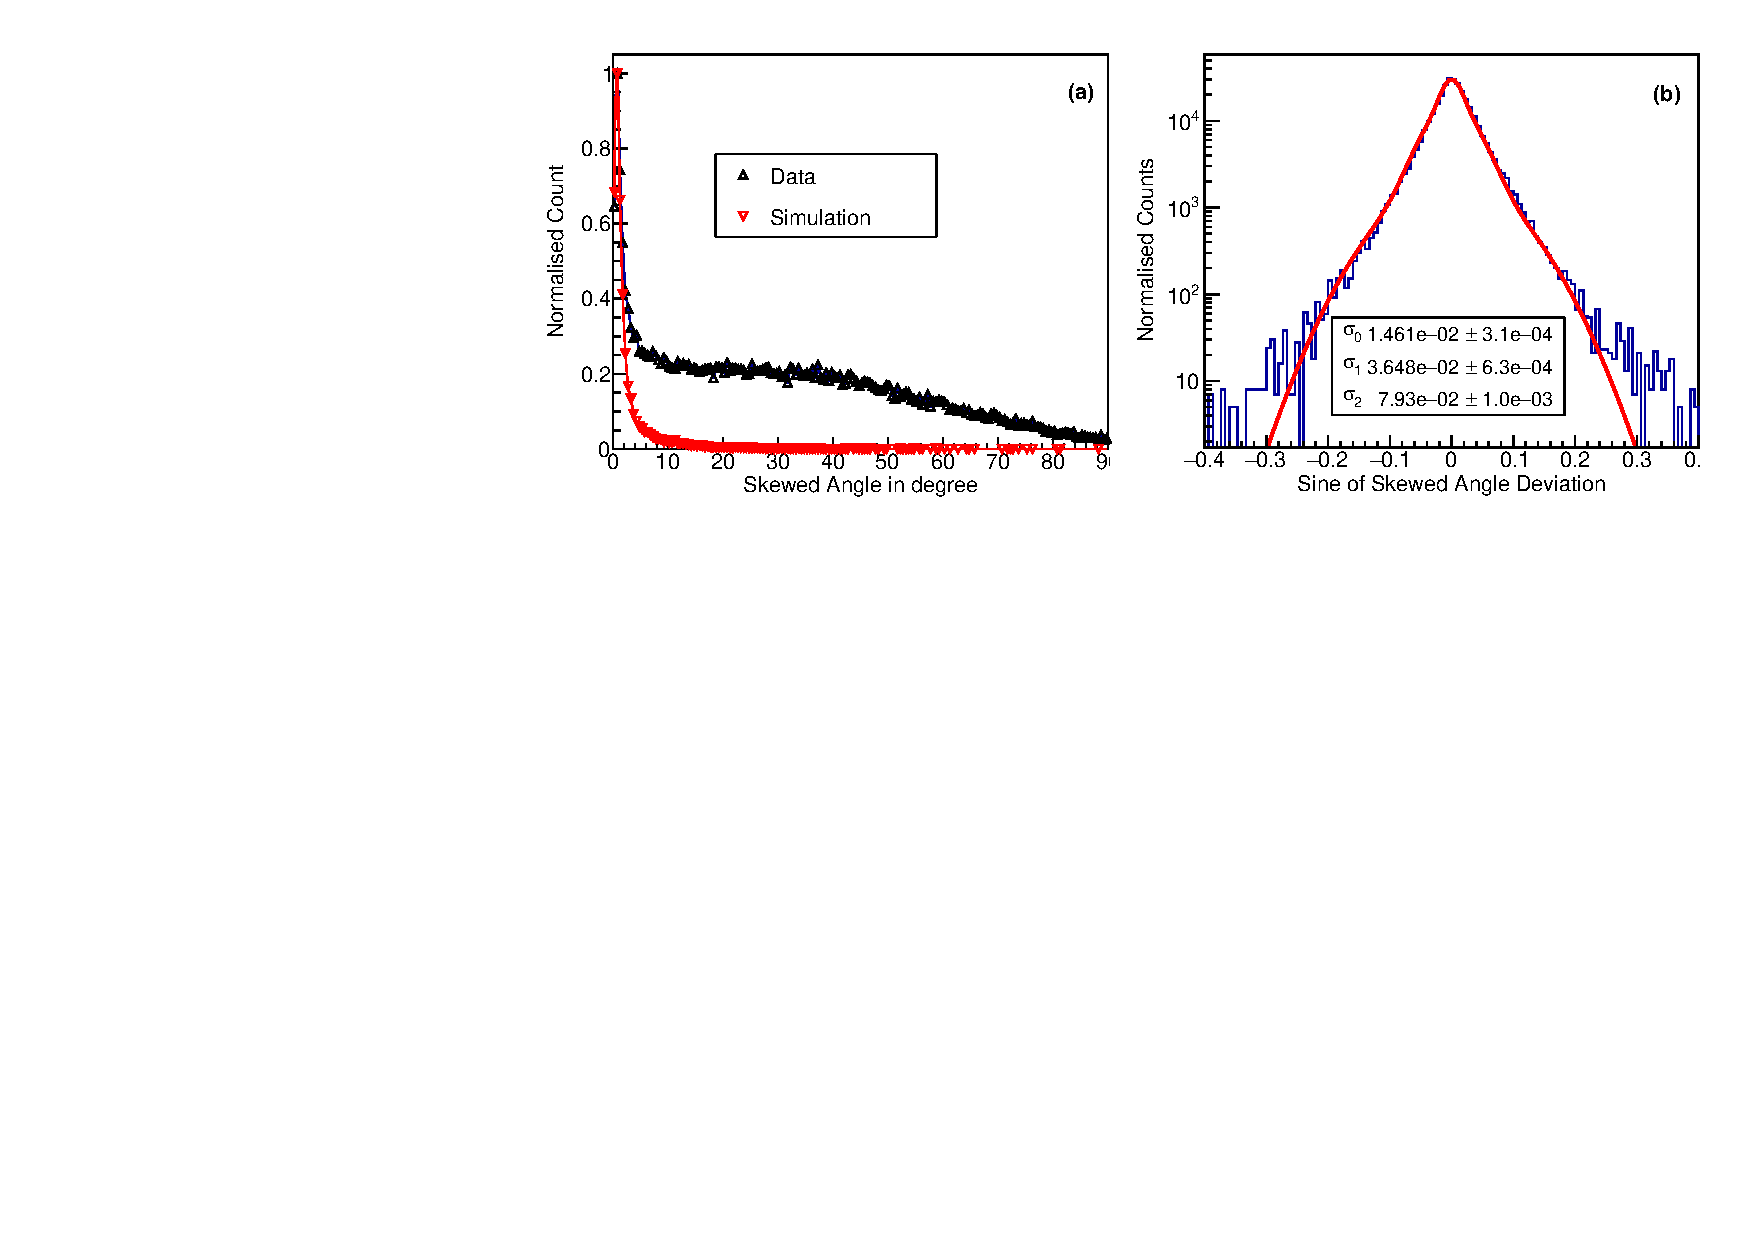
\includegraphics[width=0.9\textwidth]{skewed_compare_reso_2plot_full.pdf}
  \end{figure}
\end{frame}

\begin{frame}
  \frametitle{Multiple Tracks: Timing}
  \begin{itemize} %\itemsep -1pt
  \item Time difference between tracks (a) before and (b) after rejecting non-parallel tracks are shown in the plots.
  \end{itemize}
  \begin{figure}[!h]
    \vspace{-8pt}
    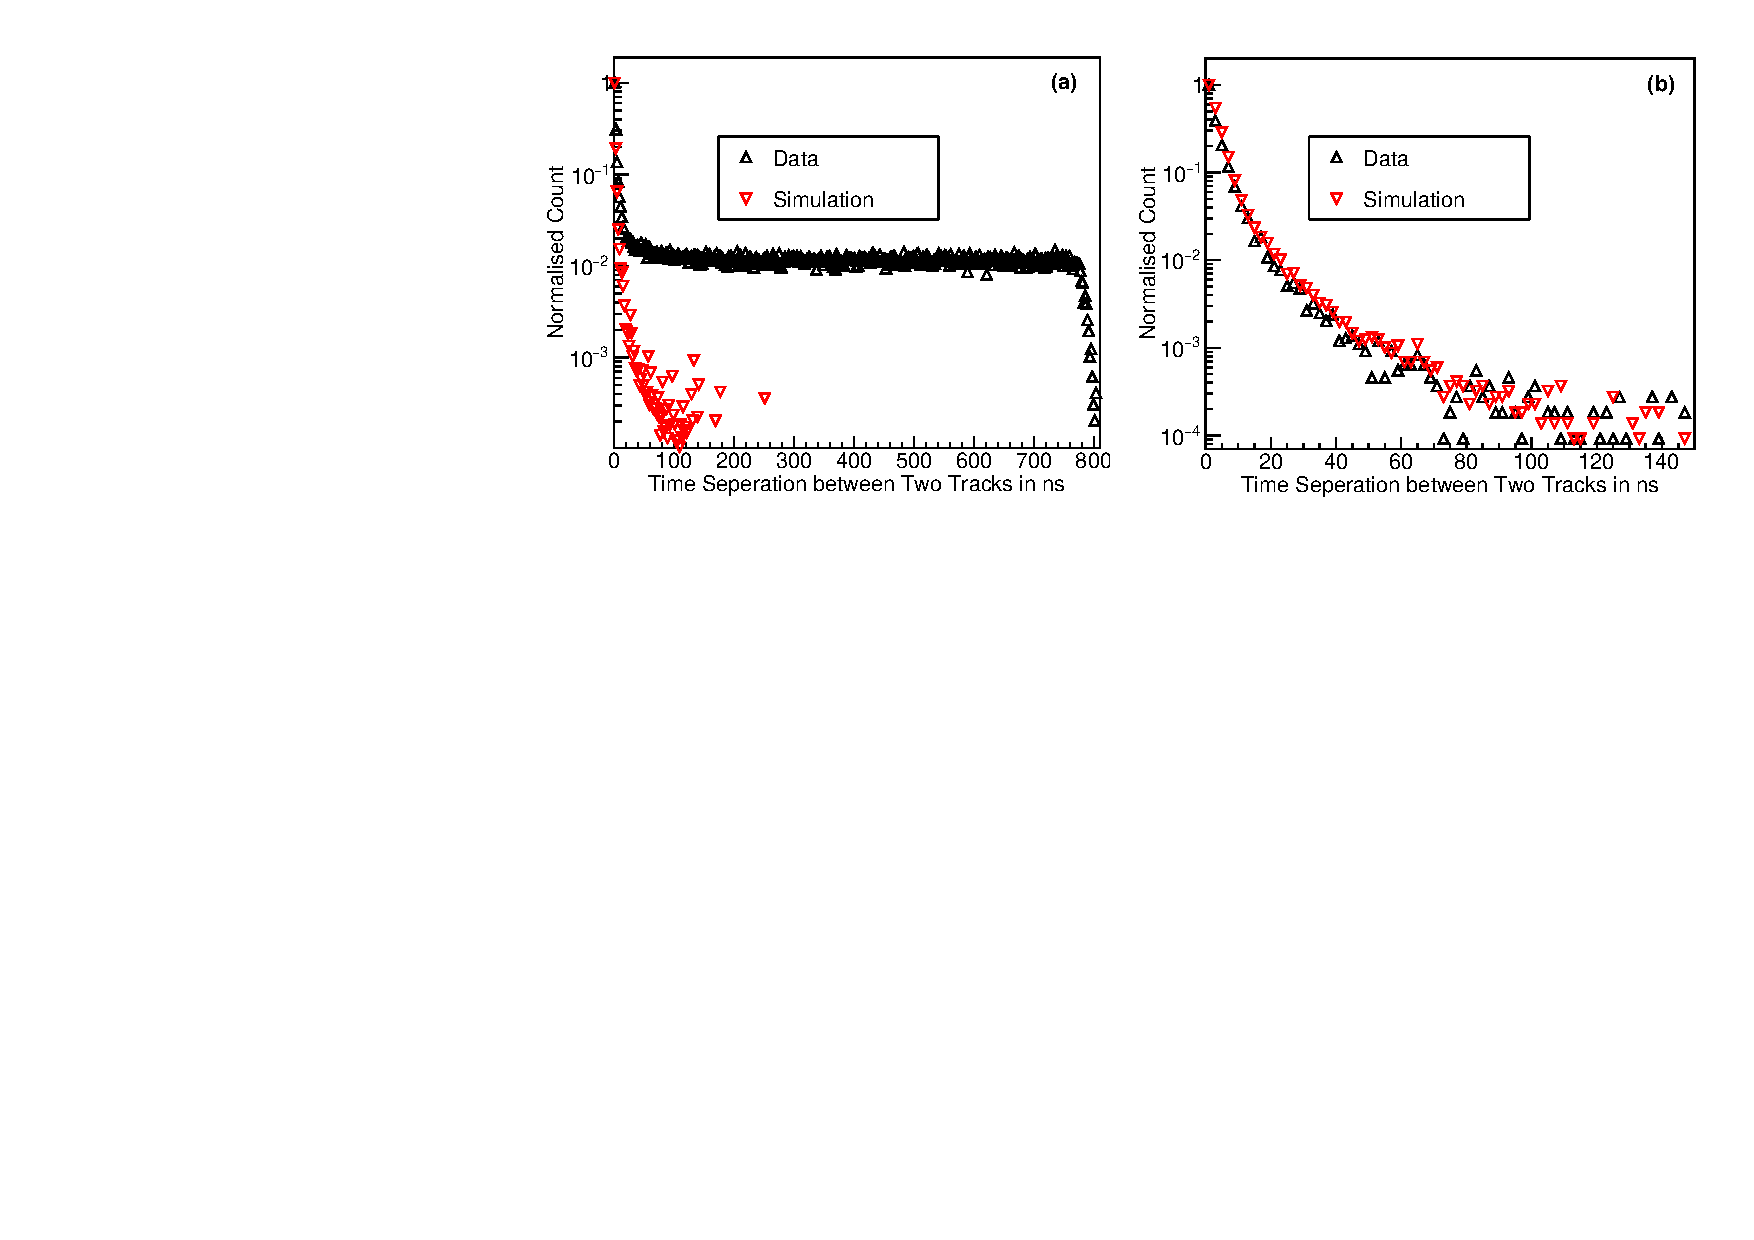
\includegraphics[width=0.9\textwidth]{time_diff_compare_all.pdf}
    \vspace{-8pt}
  \end{figure}
  \begin{itemize} %\itemsep -1pt
  \item This confirms that the rejection process is proper.
  \end{itemize}
\end{frame}

\begin{frame}
  \frametitle{Multiple Tracks: Result}
  %% \vspace{-10pt}
  \begin{itemize} \itemsep -1pt
  \item In the data, the normalised fraction of events with 2, 3 and 4
    tracks are calculated to be \mbox{$6.35\times 10^{-3}$\%},
    \mbox{$5.8\times 10^{-5}$\%} and \mbox{$2\times 10^{-6}$\%}
  \item The normalised fraction of the events containing 2, 3 and 4
    tracks are also calculated from the CORSIKA simulation for
    different cosmic primaries (H, He, C, Si and Fe) and with
    different physics packages (QGSJET-II-04 and QGSJET01d).
  \end{itemize}
  \begin{table}[btbp]
    \resizebox{\textwidth}{!}{
      \begin{tabular}{|c|cccccc|} \hline
        No of   &  H      & He       & C     & O    & Si      & Fe   \\  \cline{2-7}
        Tracks  & \multicolumn{6}{c|}{QGSJET-II-04}                 \\ \hline
        2      & $2.19\pm 0.12\times 10^{-5}$  & $4.71\pm 0.19\times 10^{-5}$ & $1.21\pm 0.02\times 10^{-4}$ & $1.61\pm 0.02\times 10^{-4}$ & $2.42\pm 0.02\times 10^{-4}$ & $4.58\pm 0.03\times 10^{-4}$ \\
        3      & $1.02\pm 0.12\times 10^{-7}$ & $3.04\pm 0.17\times 10^{-7}$ & $1.78\pm 0.05\times 10^{-6}$  & $3.11\pm 0.06\times 10^{-6}$ & $5.57\pm 0.08\times 10^{-6}$ & $1.61\pm 0.02\times 10^{-5}$ \\
        4      & $1.61\pm 0.65\times 10^{-9}$ & $8.80\pm 2.46\times 10^{-9}$ & $5.83\pm 0.47\times 10^{-8}$  & $1.12\pm 0.07\times 10^{-7}$ & $2.35\pm 0.11\times 10^{-7}$ & $1.02\pm 0.03\times 10^{-6}$ \\
        \hline
        & \multicolumn{6}{c|}{QGSJET01d}                     \\ \hline
        2      & $2.14\pm 0.12\times 10^{-5}$ & $4.74\pm 0.13\times 10^{-5}$ & $1.19\pm 0.02\times 10^{-4}$  & $1.52\pm 0.02\times 10^{-4}$ & $2.50\pm 0.02\times 10^{-4}$ & $4.56\pm 0.03\times 10^{-4}$ \\
        3      & $9.13\pm 1.22\times 10^{-8}$ & $3.91\pm 0.18\times 10^{-7}$ & $1.90\pm 0.04\times 10^{-6}$  & $3.14\pm 0.08\times 10^{-6}$ & $6.19\pm 0.07\times 10^{-6}$ & $1.65\pm 0.02\times 10^{-5}$ \\
        4      & $0.75\pm 0.38\times 10^{-9}$& $6.48\pm 1.38\times 10^{-9}$ & $6.00\pm 0.43\times 10^{-8}$  & $1.07\pm 0.07\times 10^{-7}$ & $3.39\pm 0.11\times 10^{-7}$ & $1.16\pm 0.03\times 10^{-6}$ \\ \hline
    \end{tabular}}
  \end{table}
  %GMA moved to next page
%  Combined ratio is 0.40\,:\,0.28\,:\,0.18 including all cosmic
%  primaries.\\
%  Notable discrepancy between observation and simulation.\\
%  \url{DOI:10.1007/s10686-020-09685-6} \url{arXiv:1908.04589}
\end{frame}
%GMA : Not clear in the above moge the follwing in a new page, where 
% first put your table 3.2 from the thesis

\begin{frame}
  \frametitle{Multiple Tracks: Result}
  All the normalised fraction, calculated for
  different cosmic primaries are summed with weights where the
  abundances in the primary composition are
  used as the weights.  
  \begin{table}[btbp]
    \centering
    \resizebox{\textwidth}{!}{\begin{tabular}{|c|ccc|} \hline
      No of Tracks &  Data &   QGSJET-II-04     &  QGSJET01d \\ \hline
      2         & $6.35\pm 0.05\times 10^{-5}$ & $2.35\pm 0.13\times 10^{-5}$ & $2.37\pm 0.12\times 10^{-5}$ \\
      3         & $5.82\pm 0.53\times 10^{-7}$ & $1.12\pm 0.13\times 10^{-7}$ & $1.23\pm 0.13\times 10^{-7}$ \\
      4         & $1.94\pm 0.97\times 10^{-8}$ & $3.21\pm 0.87\times 10^{-9}$ & $2.43\pm 0.50\times 10^{-9}$ \\ \hline
    \end{tabular}}
  \end{table}
  %% \vspace{-8pt}
  %% Combined ratio is 0.40\,:\,0.28\,:\,0.18 including all cosmic
  %% primaries.\\
  Result shows discrepancy between the observed data and 
  predictions from cosmic ray particle spectrum, the CORSIKA and
  finally the GEANT4 simulation.\\
  %% Notable discrepancy between observation and simulation.
  \vspace{30pt}
  \href{https://doi.org/10.1007/s10686-020-09685-6}{DOI:10.1007/s10686-020-09685-6} \hspace{10pt} \href{https://arxiv.org/abs/1908.04589}{arXiv:1908.04589}
  %% \url{DOI:10.1007/s10686-020-09685-6} \url{arXiv:1908.04589}
\end{frame}


%% Muon Charge Ratio Part

\begin{frame}
  \frametitle{Muon Charge Ratio at Madurai}
  \begin{itemize} %\itemsep -1pt
  \item As the primary cosmic rays are dominated by the proton,
    the production of the positively charged kaons/pions/muons are
    more favoured.
  \item The principal aim of this work is to observe the charge ratio
    of muons at IICHEP Madurai and compare it with previous results.
  \item Performance of different reconstruction methods are
    also studied.
  \end{itemize}
\end{frame}

\begin{frame}
  \frametitle{Detector: mini-ICAL}
  \begin{itemize} \itemsep -1pt
  \item The detector is a magnetised iron calorimeter of 85\,tonn.
  \item It consists of 11 layers of soft-iron of size
    4\,m\,$\times$\,4\,m\,$\times$5.6\,cm.
  \item Each iron layer is assembled using 7 different parts.
    The layers are kept at 4.5\,cm separation using SS-spacers.
  \item Magnetic field of $\sim$1.4\,T is obtained in the central
    region by applying 900A of DC current through the copper coil.
  \item Resistive Plate Chambers of size 2\,m\,$\times$\,2\,m are
    used as the Active Detectors, placed in the central region
    interspersed with iron layers.
  \end{itemize}
  \vspace*{-5pt}
  \begin{figure}[h!]
    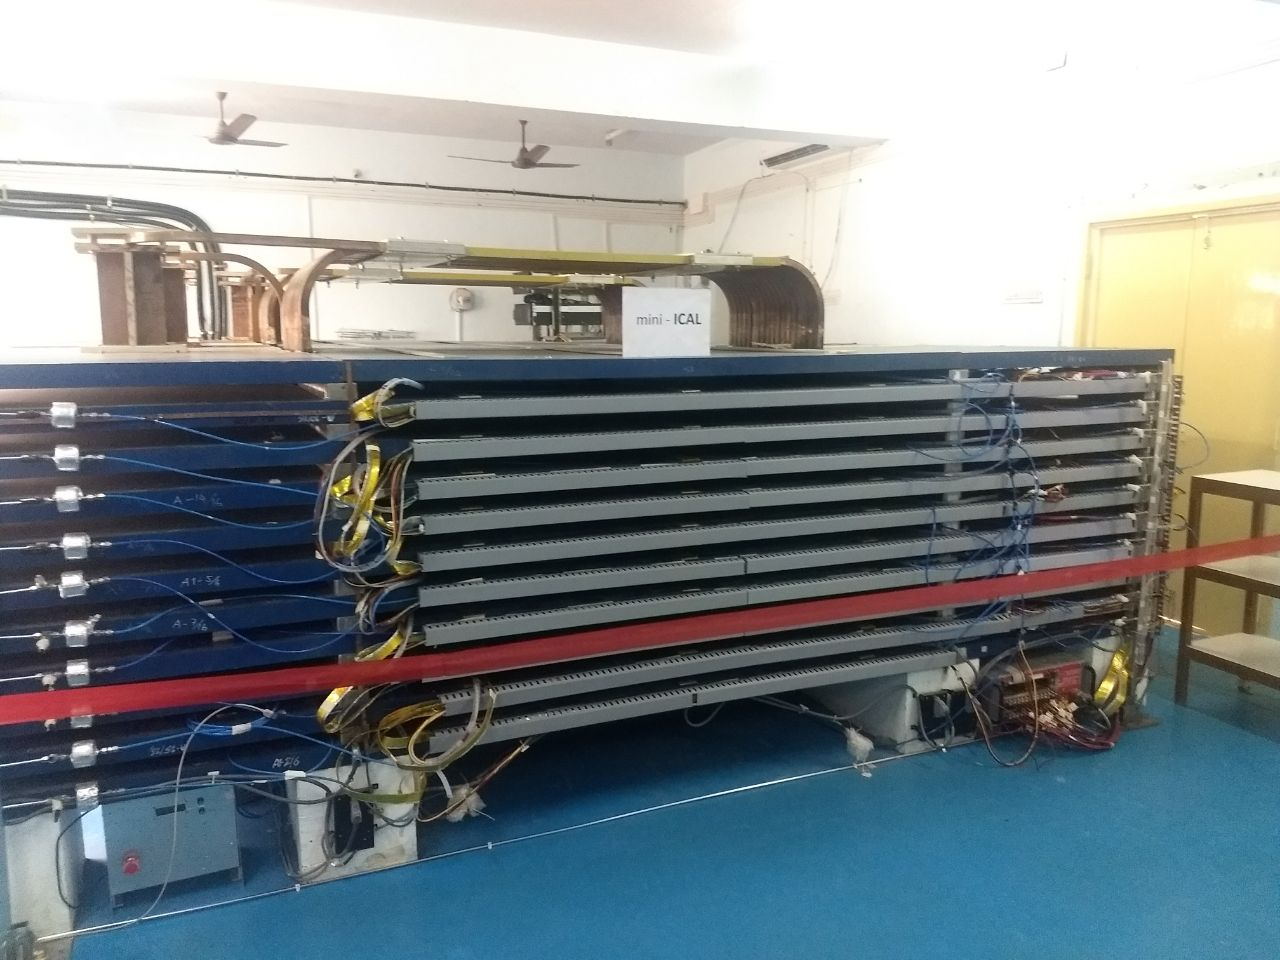
\includegraphics[width=0.45\textwidth]{micalphoto.png}
    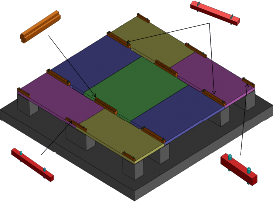
\includegraphics[width=0.45\textwidth]{miniICAL_iron_block.pdf}
  \end{figure}
\end{frame}

\begin{frame}
  \frametitle{mini-ICAL: Magnetic Field}
  \vspace*{-5pt}
  \begin{figure}[h!]
    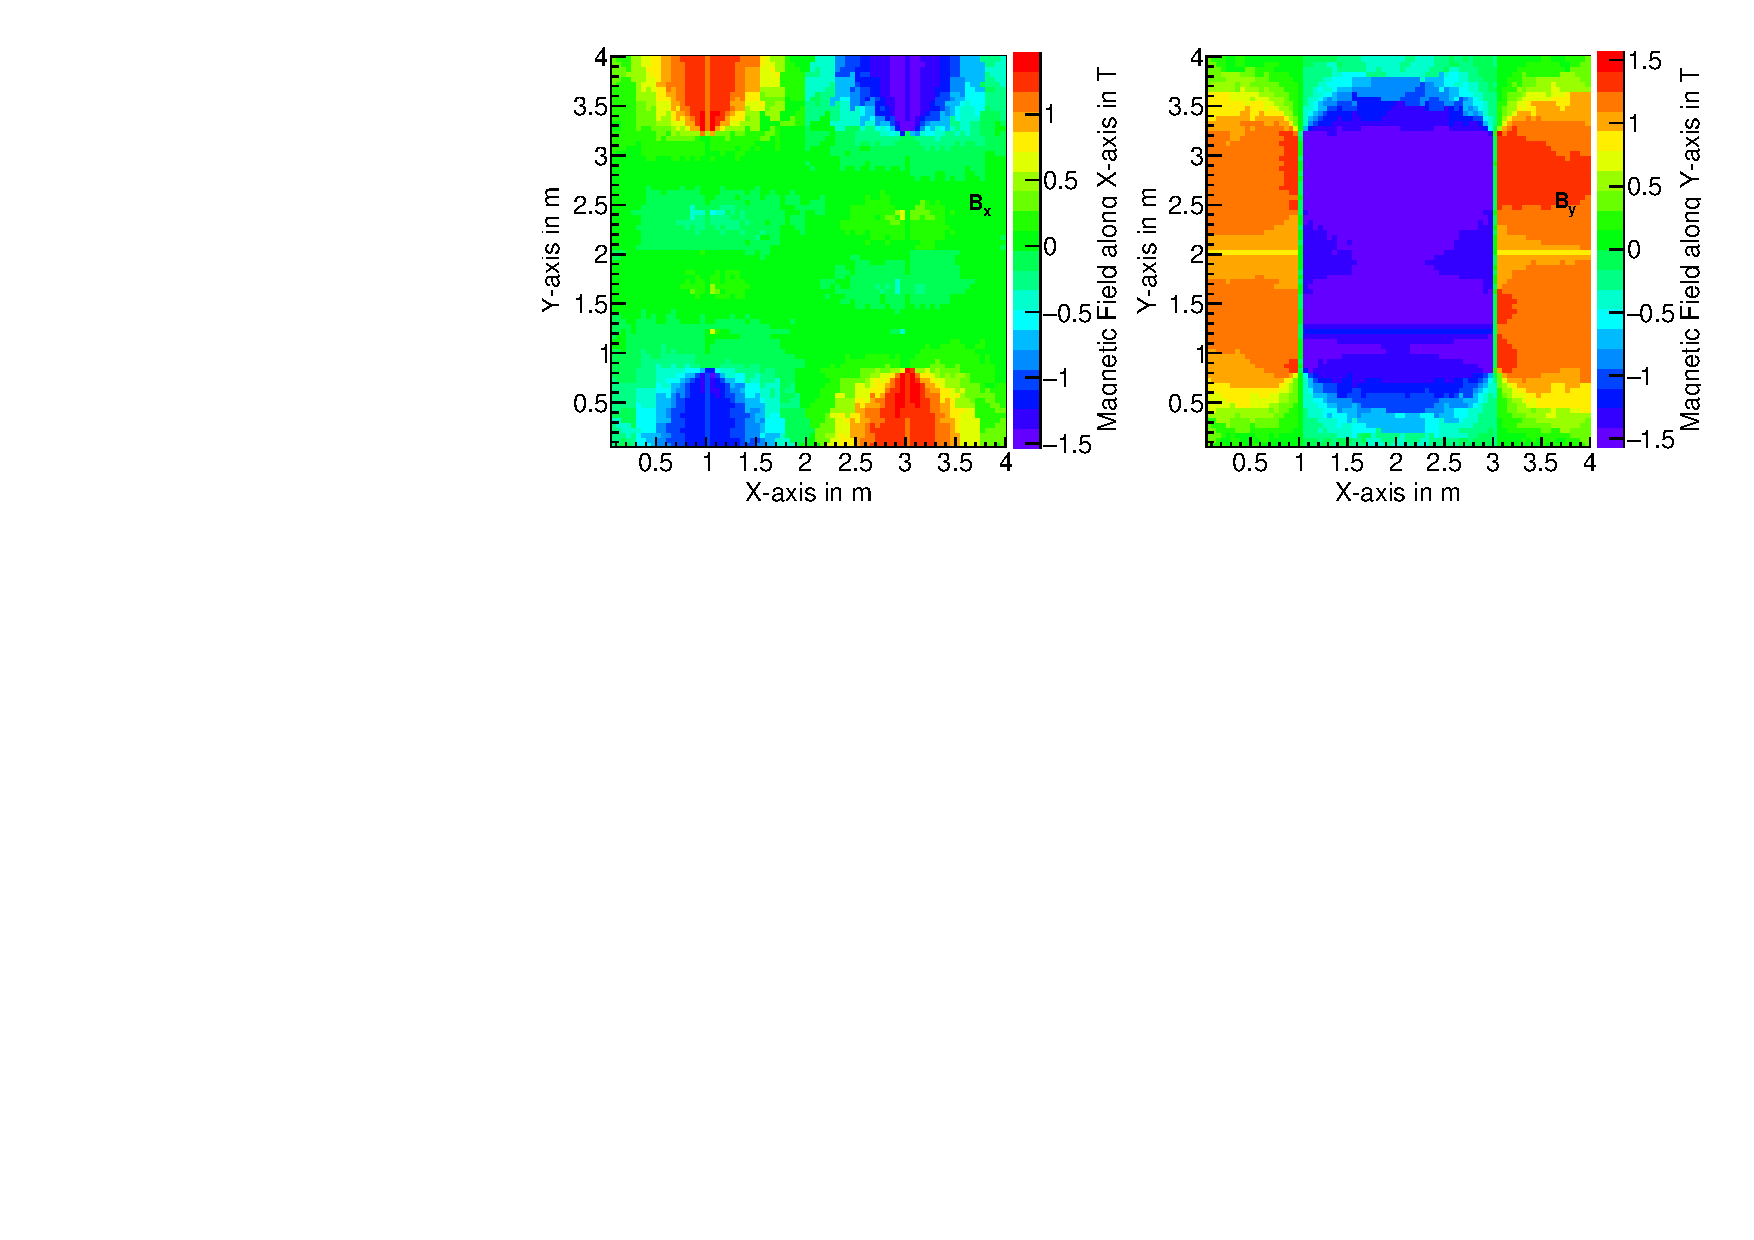
\includegraphics[width=1.0\linewidth]{mag_field_mICAL.pdf}
  \end{figure}
  \vspace*{-5pt}
  \begin{itemize} %% \itemsep -1pt
  \item Magnetic Field is simulated in MAGNET2.6 Software.
  \item No magnetic field along X-axis in the central region.
  \item Uniform field along Y-axis in the central region.
  \item Bending of tracks is only observed in the X-side.
  \end{itemize}
\end{frame}

\begin{frame}
  \frametitle{Muon Trajectory in mICAL: +/- Charged}
  \vspace*{-5pt}
  \begin{figure}[h!]
    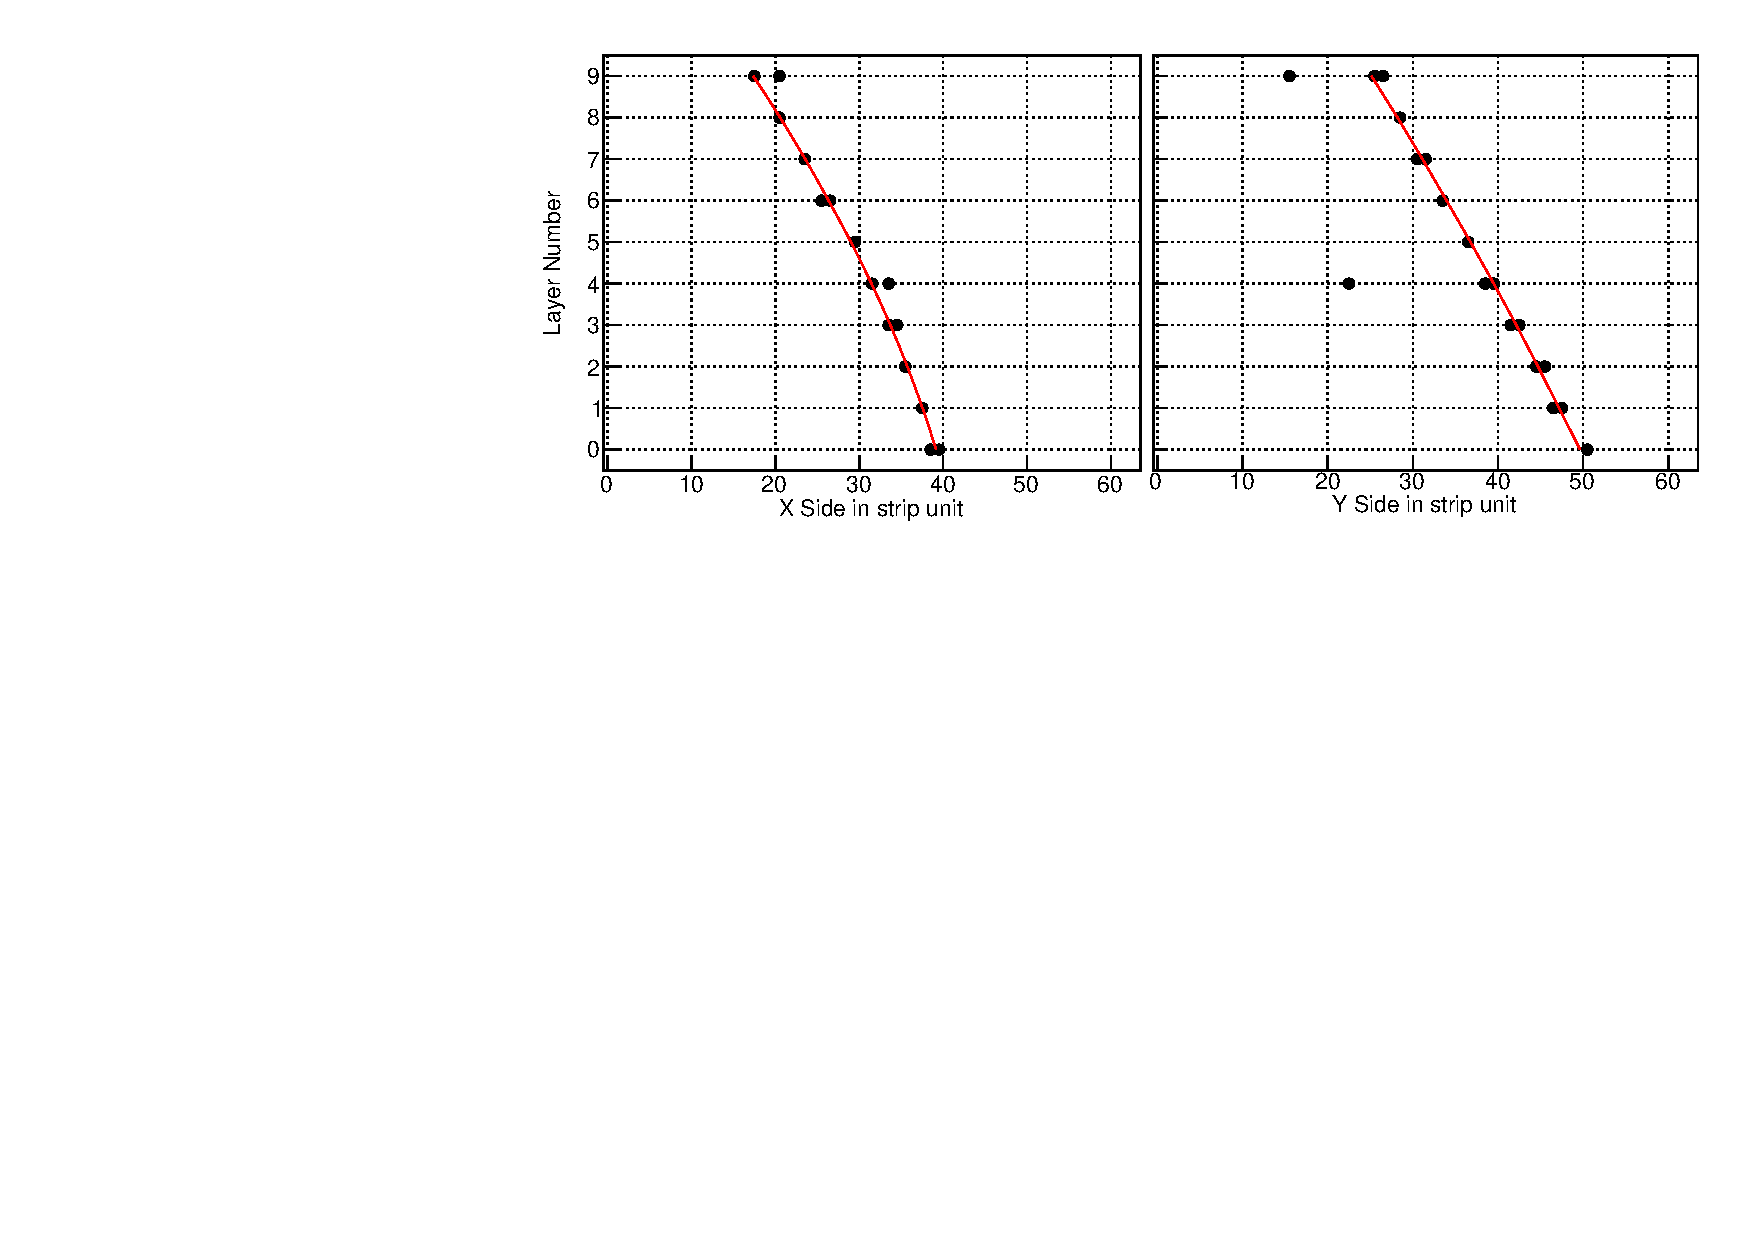
\includegraphics[width=0.82\textwidth]{Event_SNM_BRPCv4t_evtraw_20181212_091647_000157_1.pdf}
  \end{figure}
  \vspace*{-15pt}
  \begin{figure}[h!]
    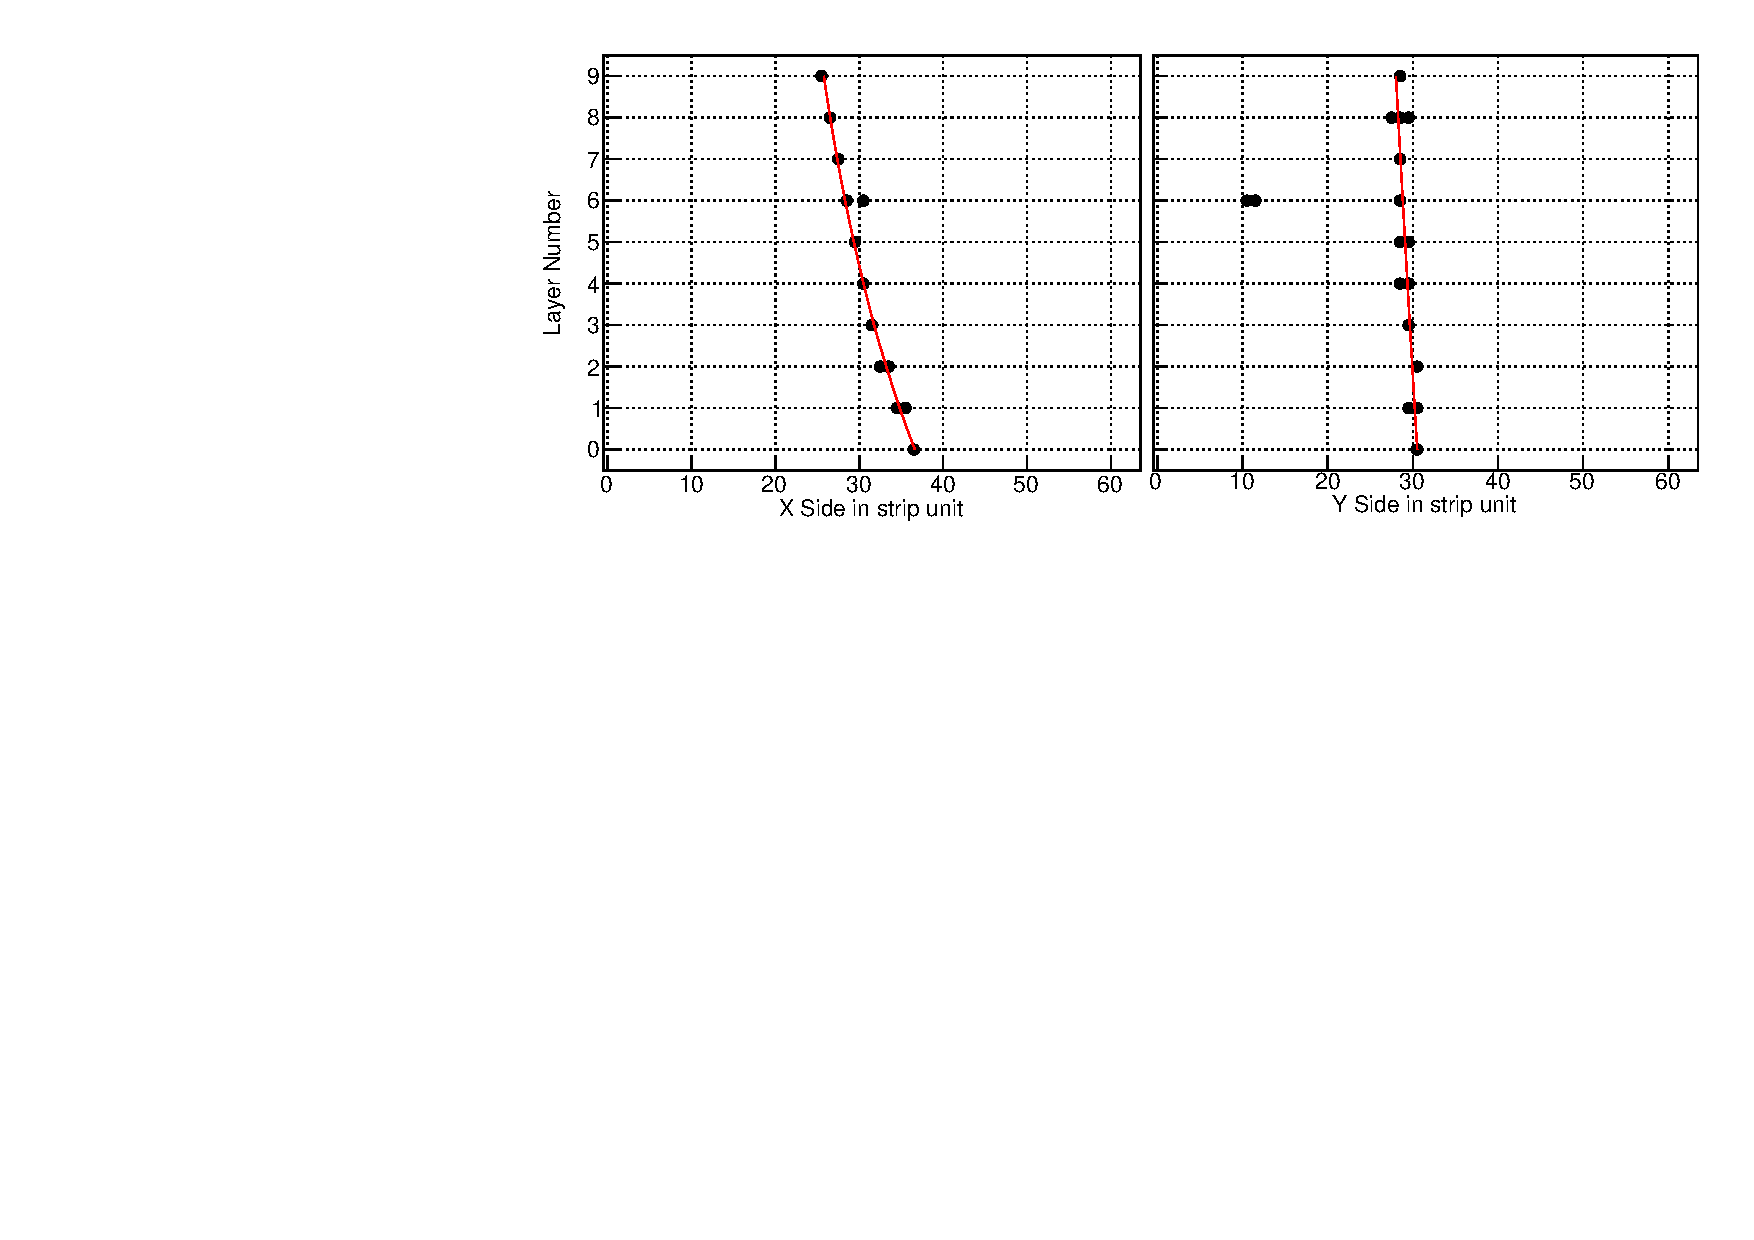
\includegraphics[width=0.82\textwidth]{Event_SNM_BRPCv4t_evtraw_20181212_091647_000045_1.pdf}
  \end{figure}
\end{frame}

\begin{frame}
  \frametitle{Simulation}
  \vspace*{-6pt}
  \begin{itemize} %% \itemsep -1pt
  \item Detector Simulation is performed using the GEANT4 toolkit
    (\url{QGSP_BERT_HP}).
  \item CORSIKA (\url{FLUKA} \& \url{SIBYLL}) generated secondaries
    are used as the input to the GEANT4 Simulation.
  \item Detector parameters (efficiency, noise and strip
    multiplicity) are incorporated in digitisation stage.
  \end{itemize}
  \vspace*{-5pt}
  \begin{figure}[h!]
    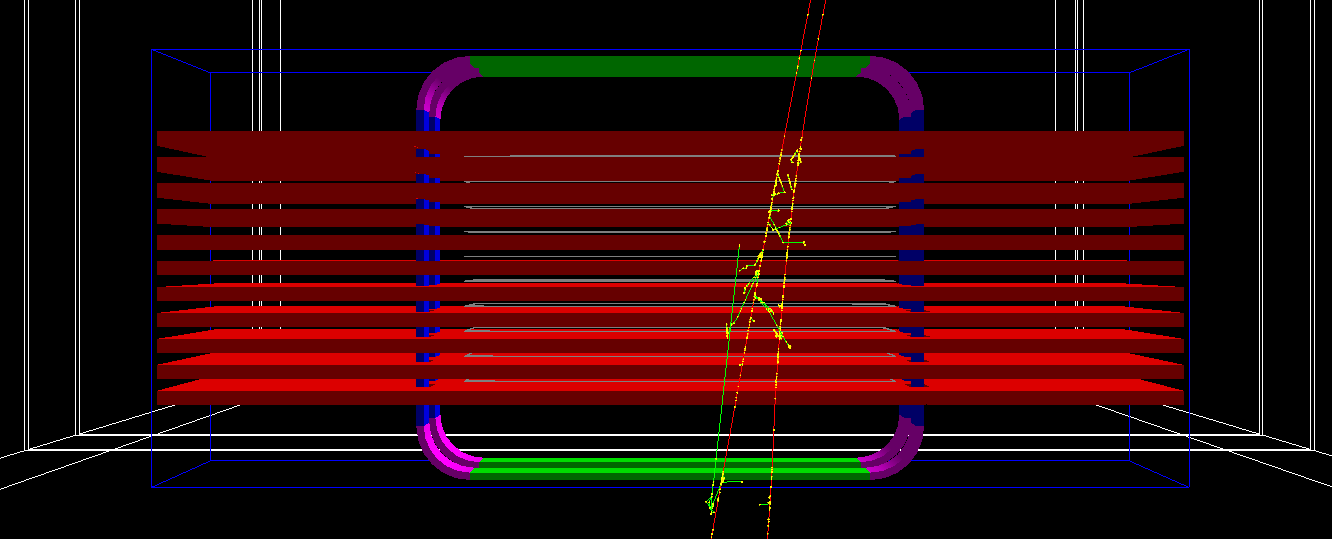
\includegraphics[width=0.99\linewidth]{mical_view.png}
  \end{figure}
  \vspace*{-9pt}
%GMA  \begin{itemize} %% \itemsep -1pt
%  \item The simulated and recorded events are then reconstructed
%    for momentum using the following methods.
%  \end{itemize}
\end{frame}

\begin{frame}%% [shrink]
  \frametitle{Momentum Reconstruction}
  %GMA added here
  The simulated and recorded events are then reconstructed
  for momentum using the following methods.
  %% Different techniques for the reconstruction :
  \begin{itemize} %% \itemsep -1pt
  \item {\bf Circle-Fit:} X-side and Y-side projections are fitted with
    Circle and Straight line, respectively. Momentum and position of
    incidence is estimated from the curvature of the circle fit.
  \item {\bf Grid-Search:} The particle is propagated in the detector
    medium using the 4$^{th}$-order Runge-Kutta-Nystrom initiated with
    Circle-Fit parameters. The best fit momentum is then found using
    the method of Grid-Search.
  \item {\bf Explicit-Model Fit (using Simpson's approx.):}
    The momentum is also reconstructed
    using the Explicit-Model Fit initiated with Circle-Fit parameters.
  \item {\bf Kalman-Fit:} The momentum is again reconstructed
    using the Kalman-Fit method. Here the initial $q/p$ ratio is
    taken as zero and initial direction is estimated from the first
    two hits.
  \end{itemize}
  The events with at-least 7 layers of hits are reconstructed.
\end{frame}

\begin{frame}
  \frametitle{Reconstructed Momentum: Response}
  \vspace*{-5pt}
  \begin{figure}[h!]
    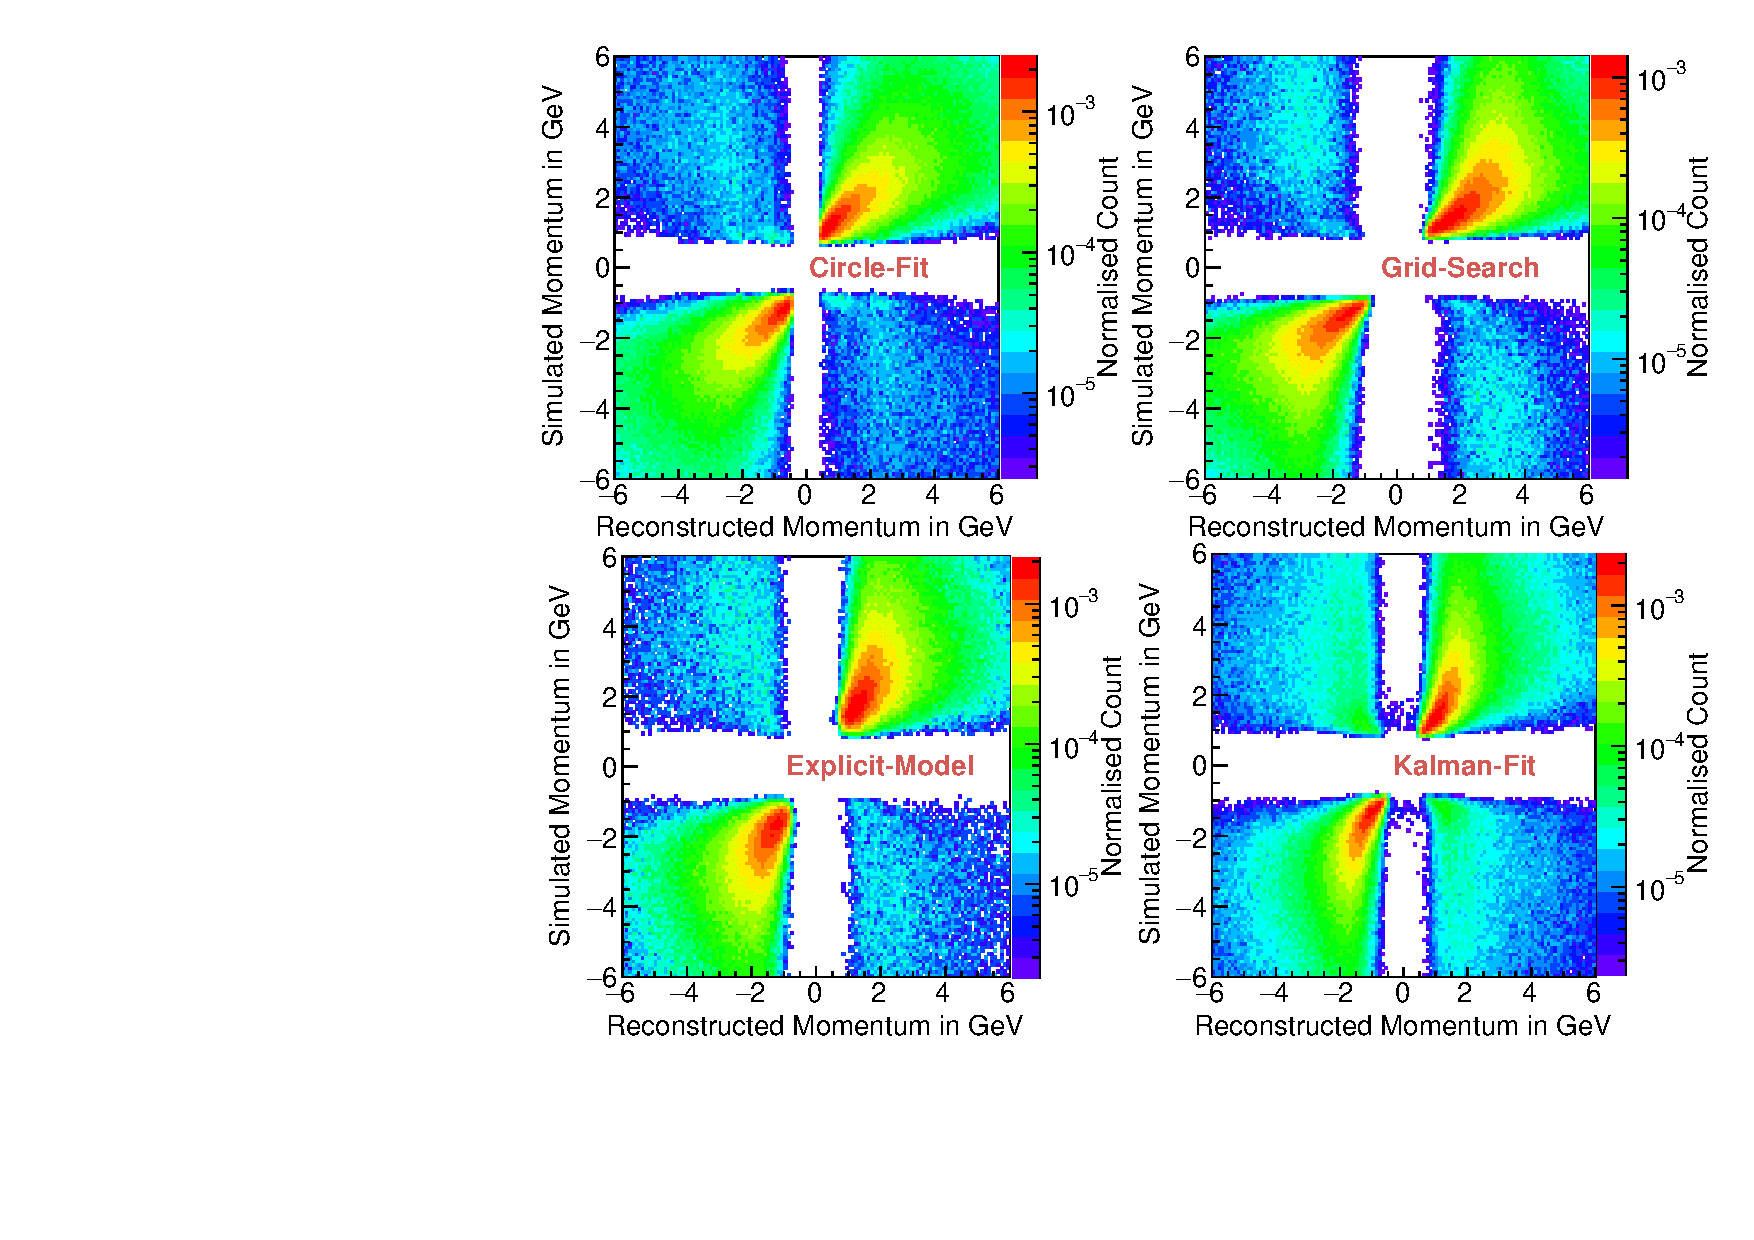
\includegraphics[width=0.8\linewidth]{responseMatrix_10Layer_All4.pdf}
  \end{figure}
\end{frame}

\begin{frame}
  \frametitle{Reconstruction Efficiency and Resolution}
  \vspace*{-12pt}
  \begin{figure}[h!]
    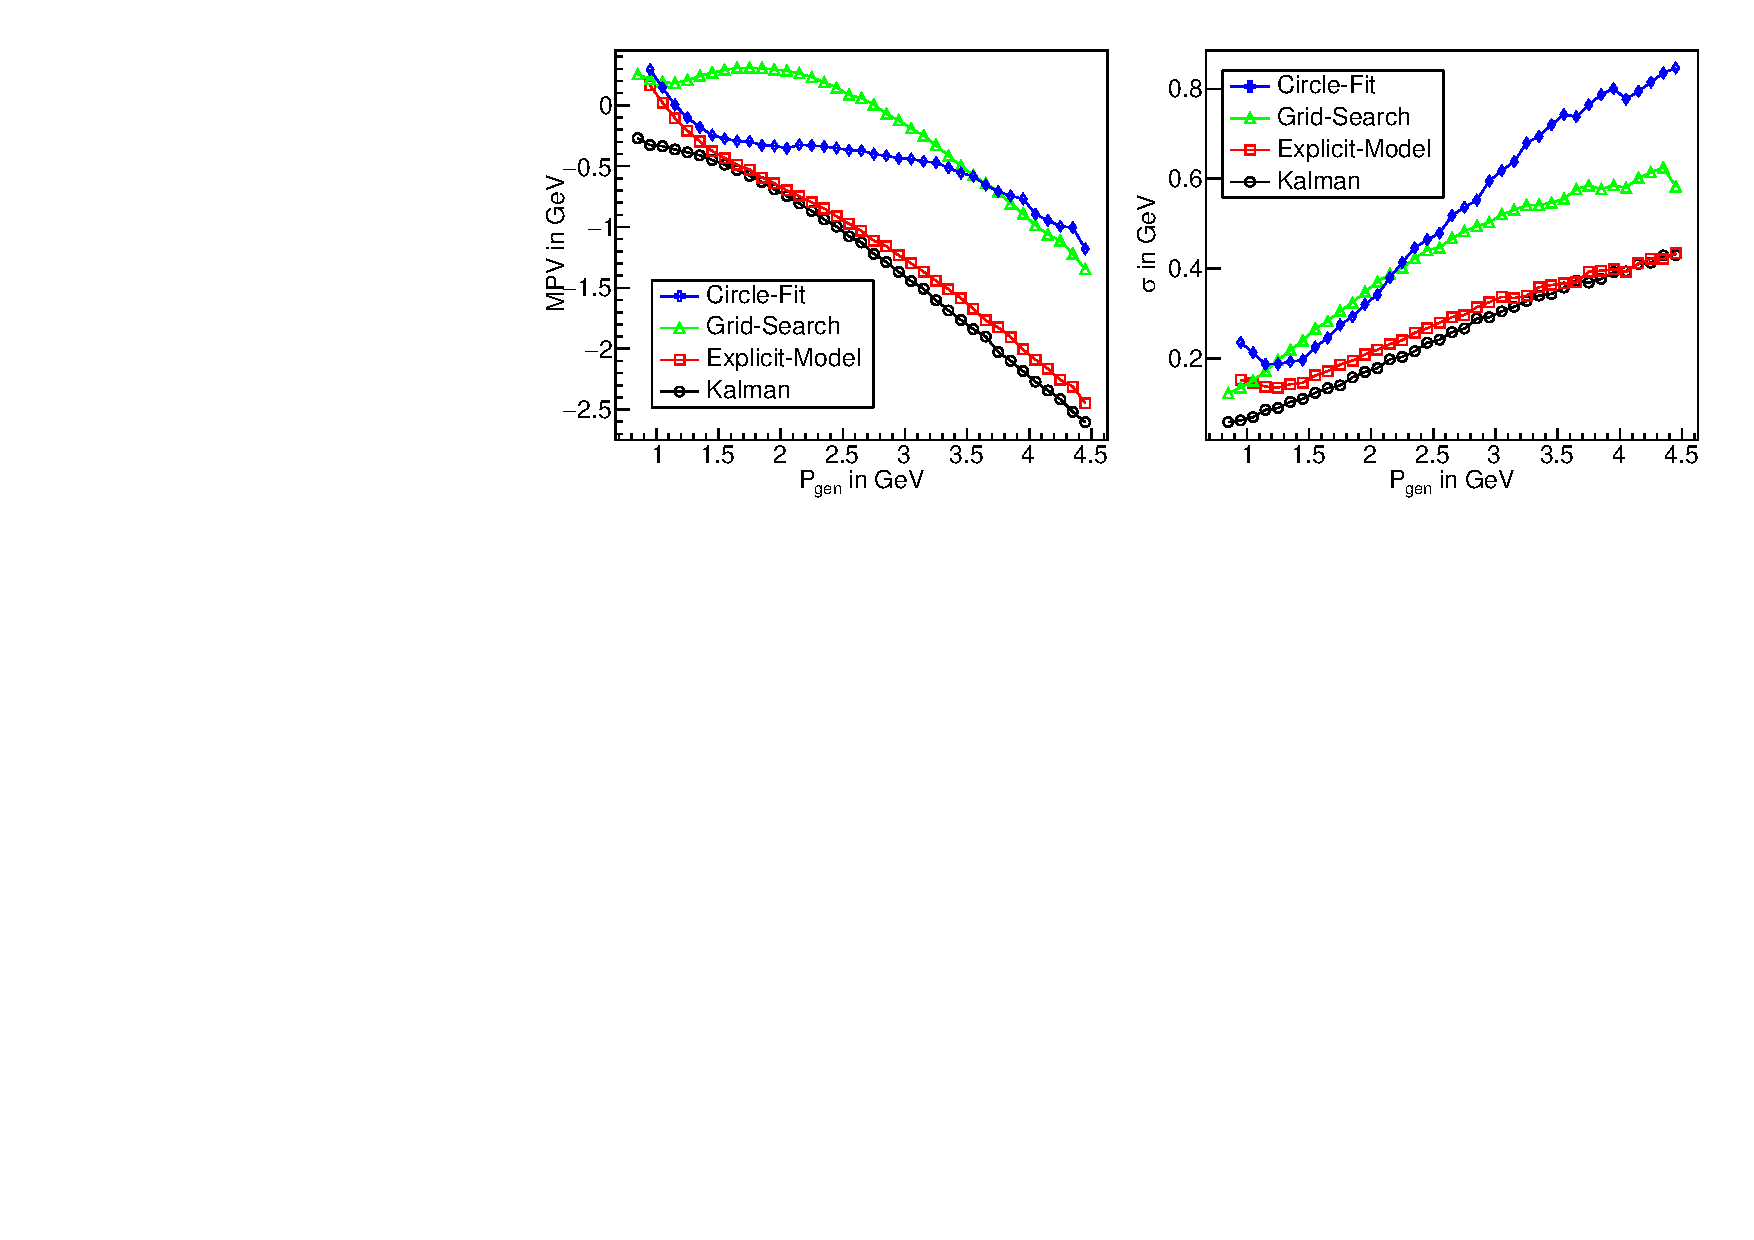
\includegraphics[width=0.72\linewidth]{GMA_mpv_sigma_All4.pdf}\\
    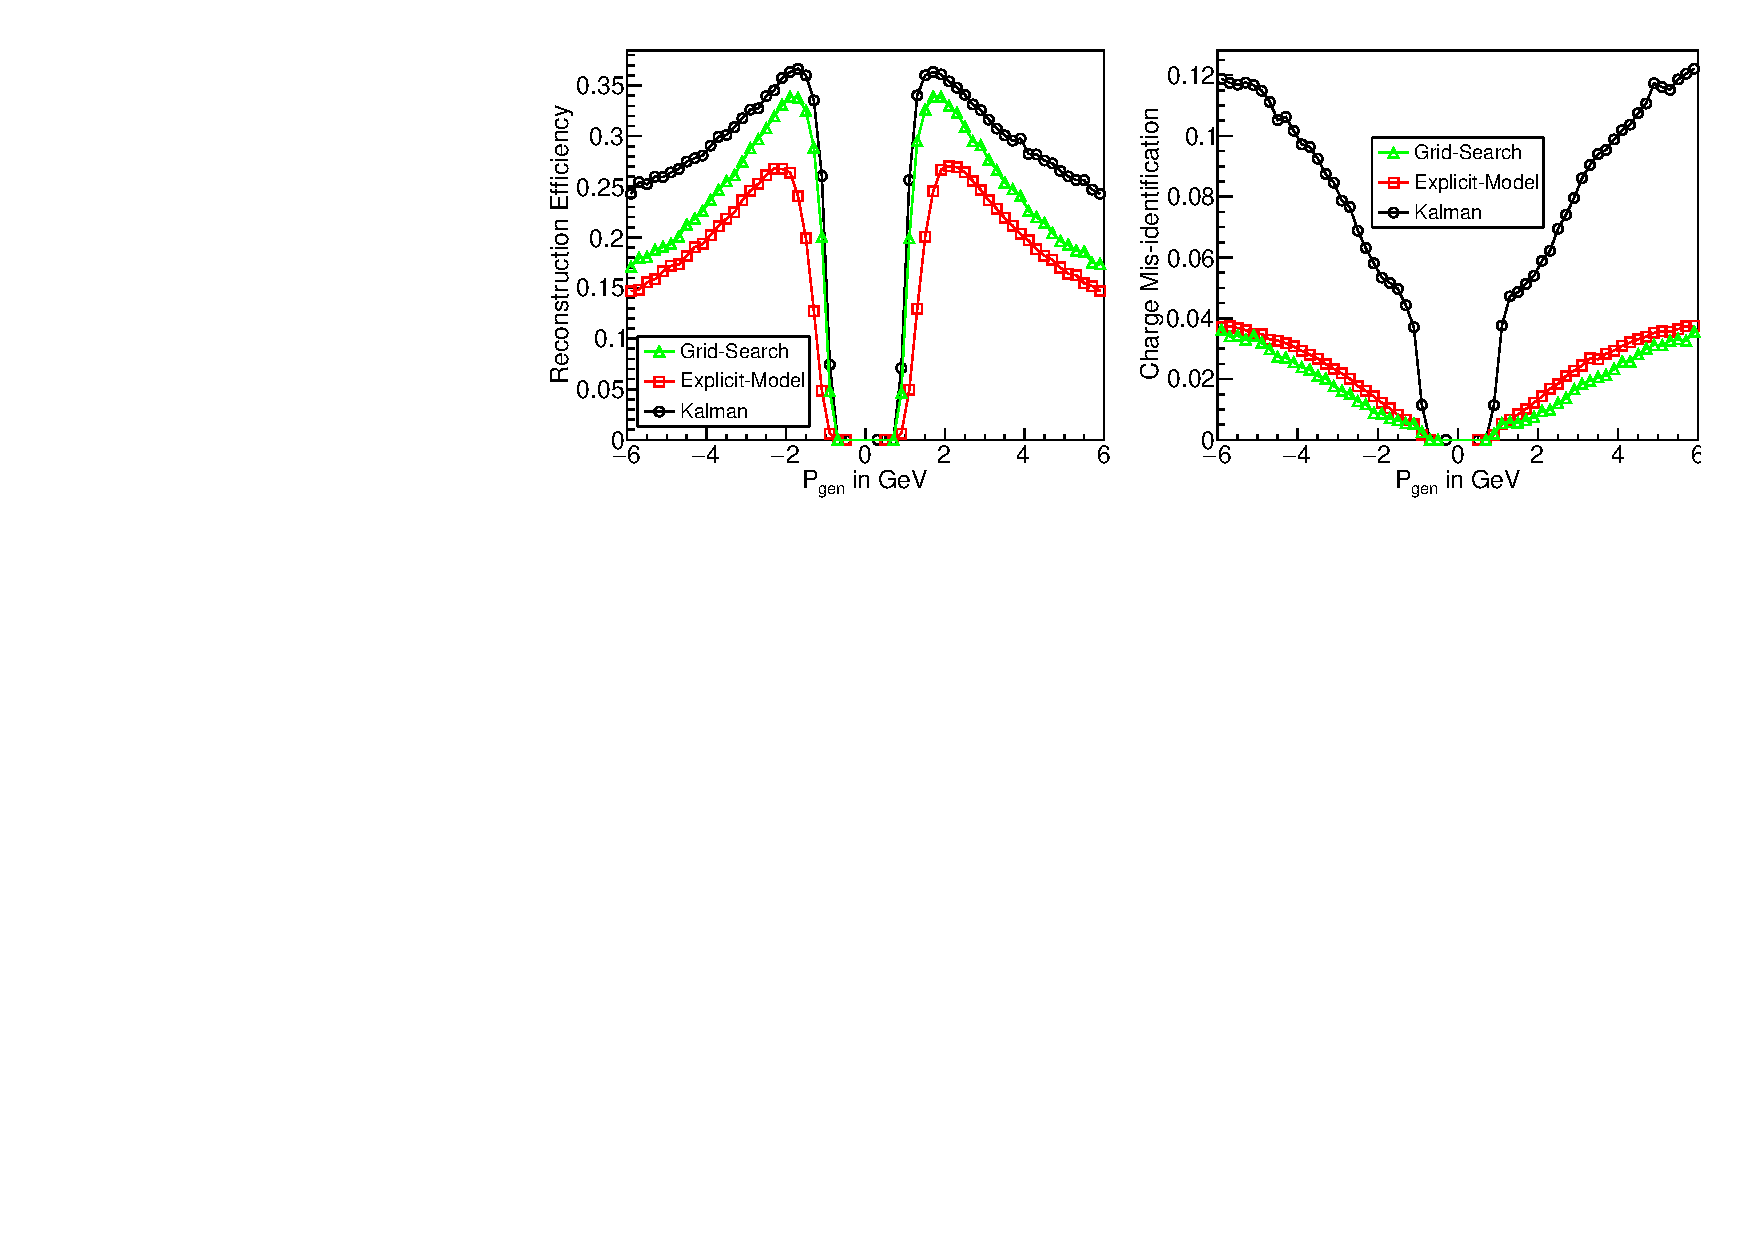
\includegraphics[width=0.72\linewidth]{GMA_effi_misId_All4.pdf}
  \end{figure}
  \vspace*{-9pt}
  Based on performance of charge mis-identification, overall momentum
  resolution and saturation of reconstructed momentum, the
  Grid-Search Method has been accepted.
\end{frame}

\begin{frame}
  \frametitle{Unfolding}
  \vspace*{-9pt}
  \begin{itemize} %% \itemsep -1pt
  \item Measured momentum is biased due to the effect of building,
    limited acceptance, resolution, etc.
    \vspace*{-9pt}
    \[{\bf A}{\bf x}+{\bf b}={\bf y}\vspace*{-9pt}\]
    where, {\bf A} is the `response', {\bf x} is the `truth'
    spectra, {\bf b} is the `background' and {\bf y} is the `measured'
    spectra.
  \item Measured momentum is unfolded to eliminate the detector's
    effect using the Iterative Bayesian Unfolding.
  \item The number of iterations required for the unfolding is
    obtained in the following. (The following is shown only for $\mu^+$,
    but it showed same result for $\mu^-$ also.)
  \end{itemize}
\end{frame}

\begin{frame}[shrink]
  \frametitle{Unfolding: Number of Iterations}
  \vspace*{-9pt}
  \begin{itemize} \itemsep -1pt
  \item A `response' is constructed with generated vs smeared
    momentum with calculated MPV and $\sigma$ values in Grid-Search.
  \item Above step is repeated with different seed, to create `truth'
    and `measured' spectra.
  \end{itemize}
  \vspace*{-9pt}
  \begin{figure}[h!]
    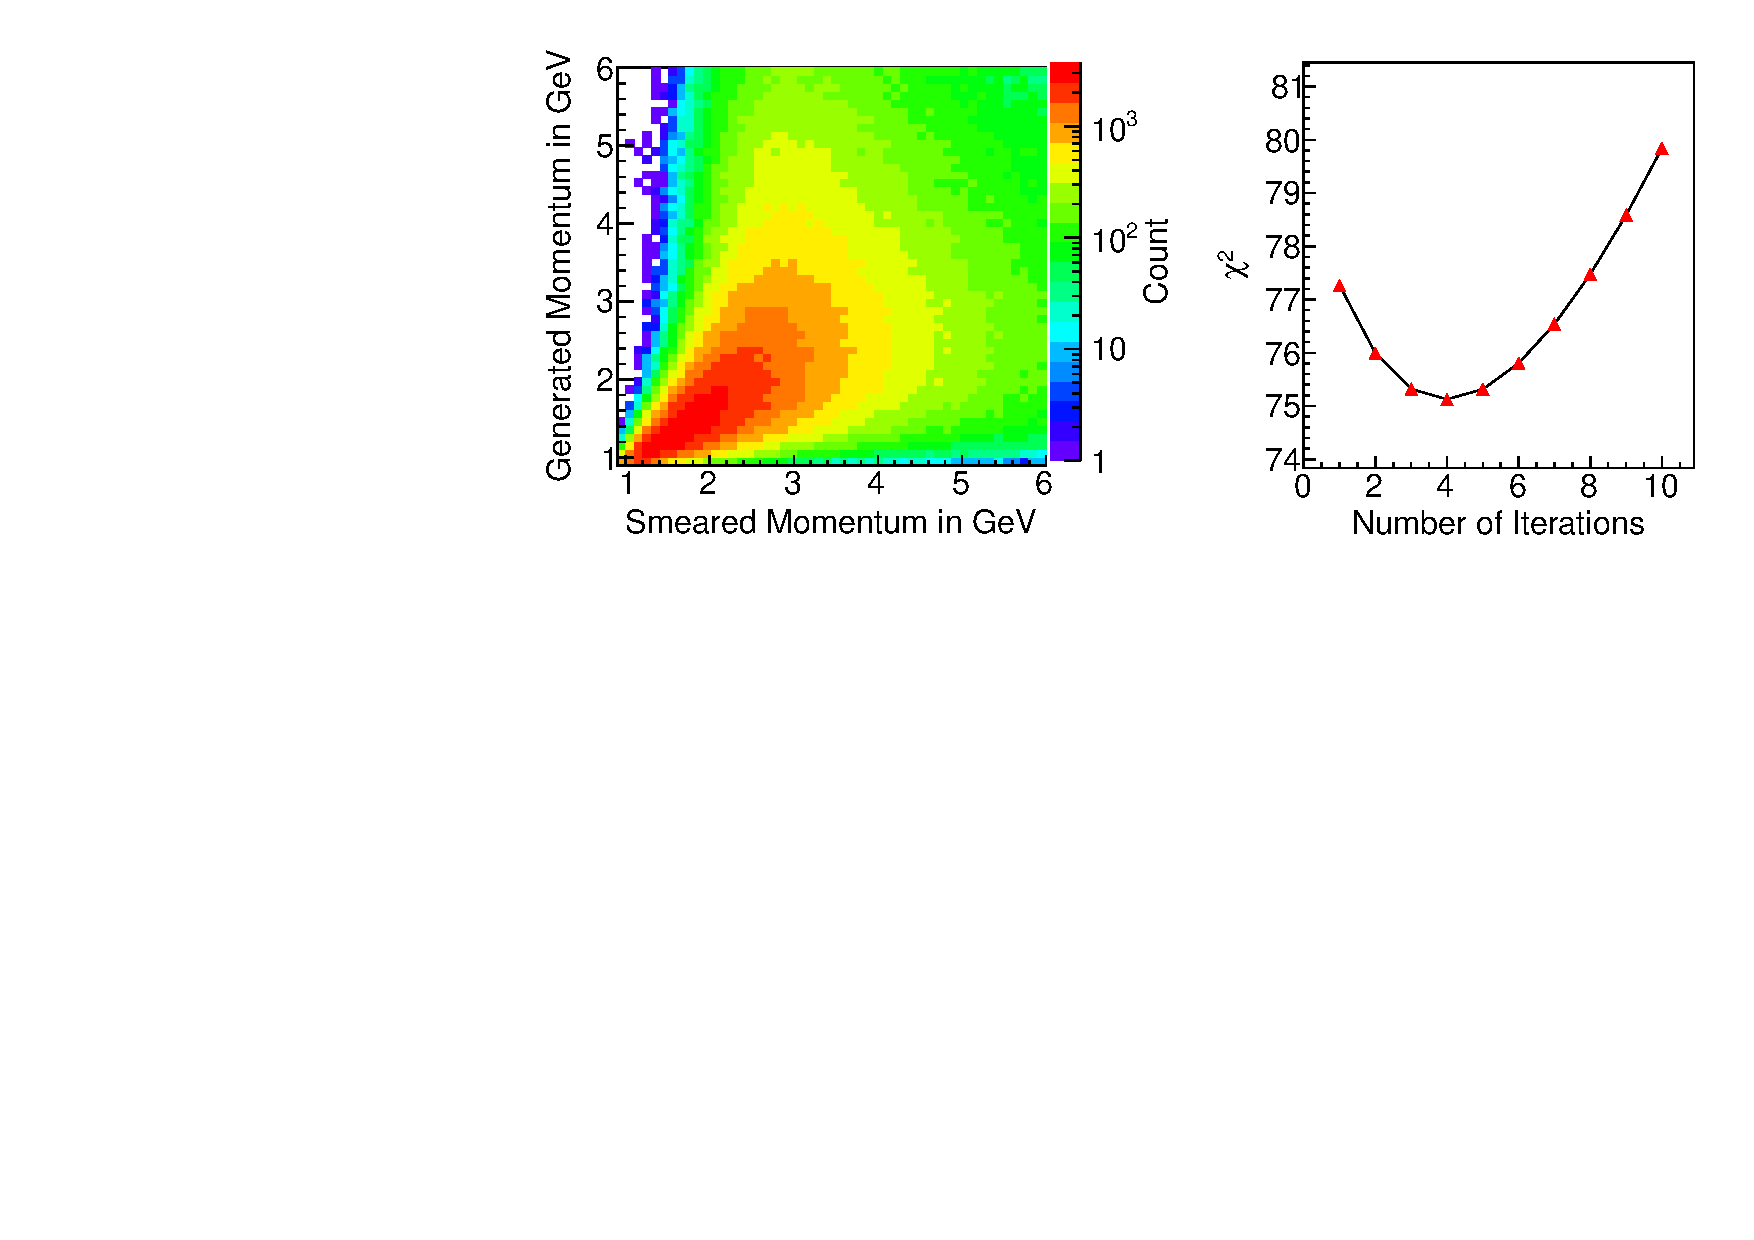
\includegraphics[width=0.72\textwidth]{ResoResponse_Grid.pdf}
  \end{figure}
  \vspace*{-9pt}
  \begin{itemize} %% \itemsep -1pt
  \item The `measured' spectra is unfolded using using the `response'
    to get back the `truth'.
  \item At iteration 4, the unfolded spectra is matching the
    closest with the generated spectra.
  \item $\chi^2$ is also minimum at iteration 4 for variation of
    20\% more or less resolution.
    %% \item The process for $\mu^-$ also returned the same result.
  \end{itemize}
\end{frame}

\begin{frame}
  \frametitle{Unfolded Momentum: Data}
  \vspace*{-9pt}
  \begin{itemize} %% \itemsep -1pt
  \item Reconstructed momentum from data is then unfolded using
    response matrix generated from GEANT4 Simulation.
  \item Background, efficiency and fake-rate in each reconstructed
    momentum bin are calculated during the unfolding.
  \item The Ratio of the number of $\mu^{+}$ to $\mu^{-}$ is then
    calculated and compared with BESS-TeV 2002.
  \end{itemize}
  \vspace*{-9pt}
  \begin{figure}[h!]
    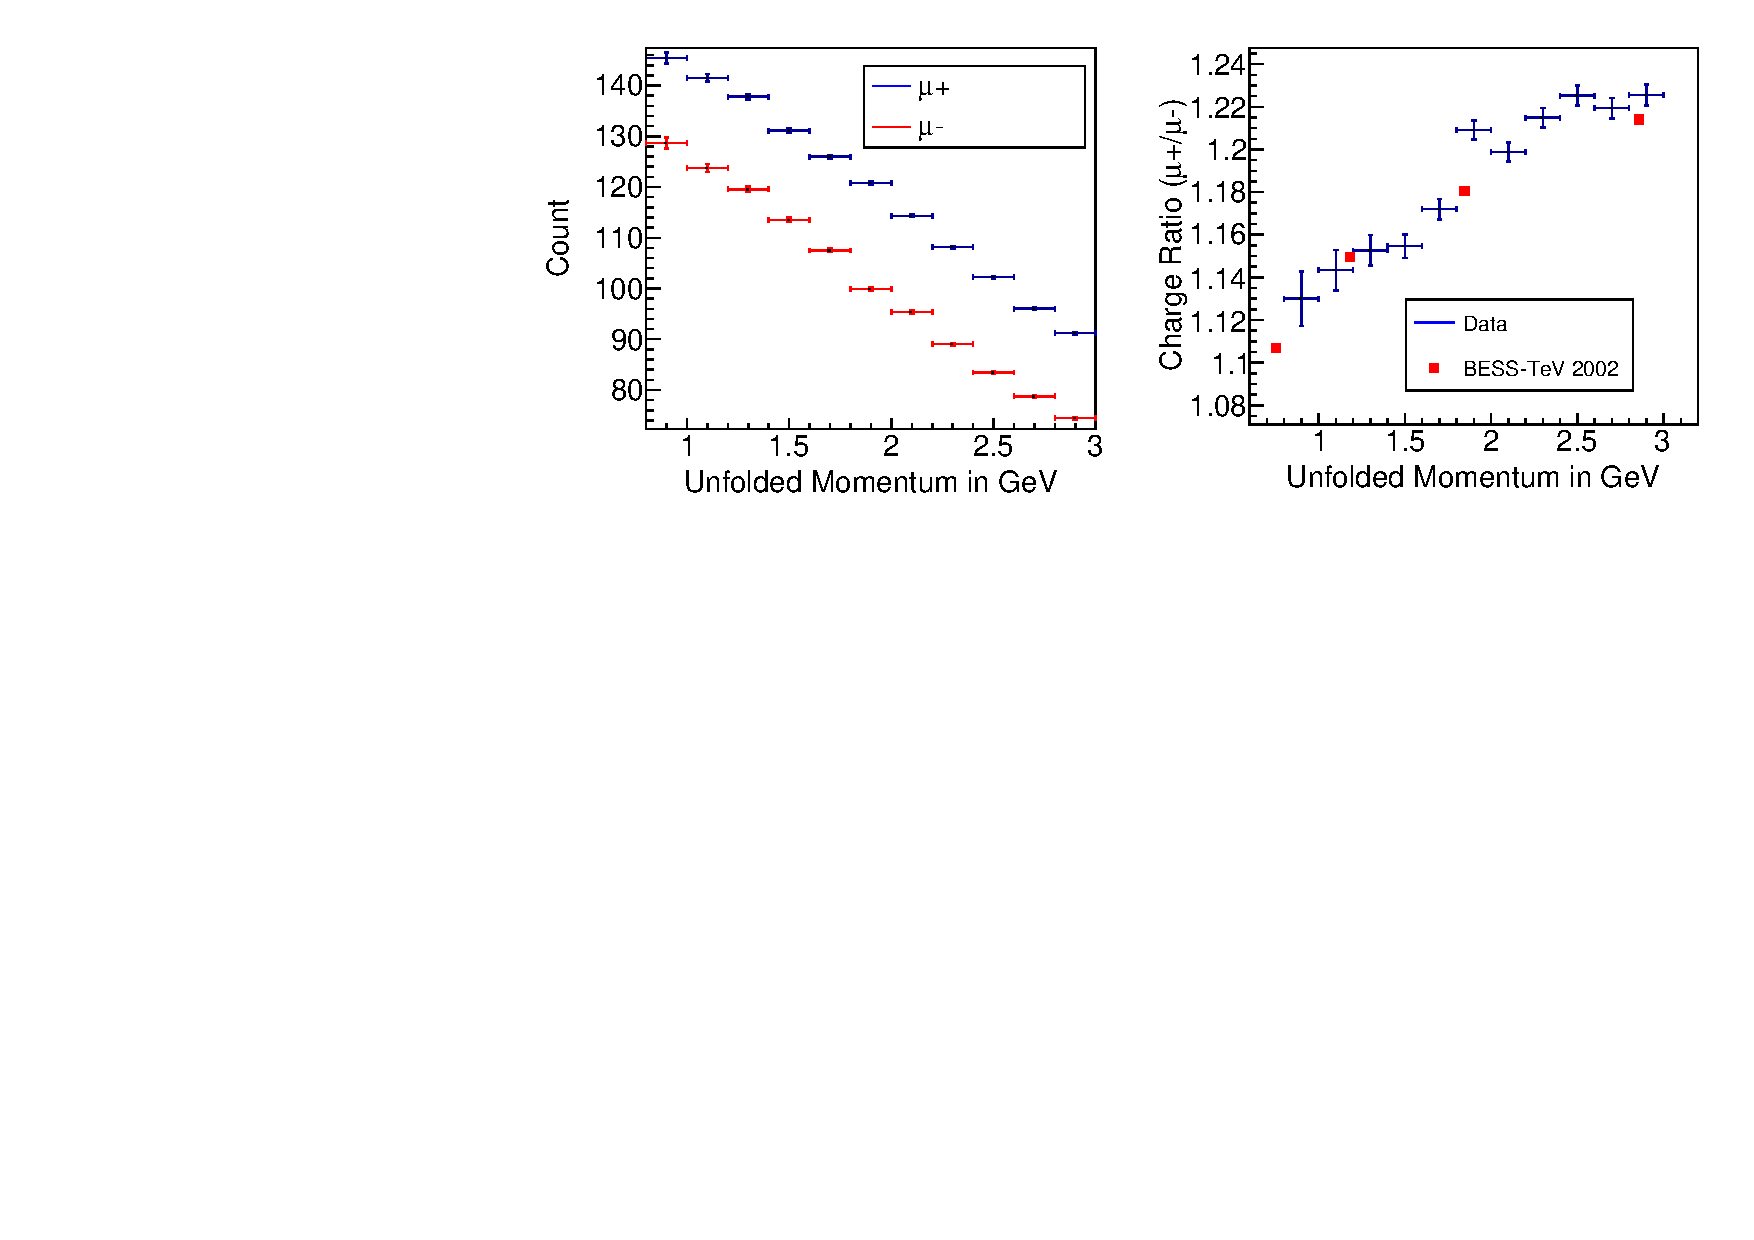
\includegraphics[width=0.8\linewidth]{UnfoldedPlot_Grid.pdf}
  \end{figure}
  \vspace*{-9pt}
  Momentum beyond 3\,GeV is not unfolded as the momentum resolution
  saturates beyond this energy.
\end{frame}

\begin{frame}
  \frametitle{Engineering Module}
  \vspace*{-6pt}
  \begin{itemize} %% \itemsep -1pt
  \item A new detector setup, named as Engineering Module
    with 20 Layers of RPCs is going to be built in the near future.
  \item GEANT4 is used to simulate events in this model.
  \item The Grid Search method gives better results for a 10 layer
    setup, but is too time consuming. Explicit track fit model is
    chosen in this case, which is expected to perform well with
    increased number of hit points.
  \item The events with more than 14 layers of hits are reconstructed.
  \end{itemize}
  \vspace*{-4pt}
  \begin{figure}[h!]
    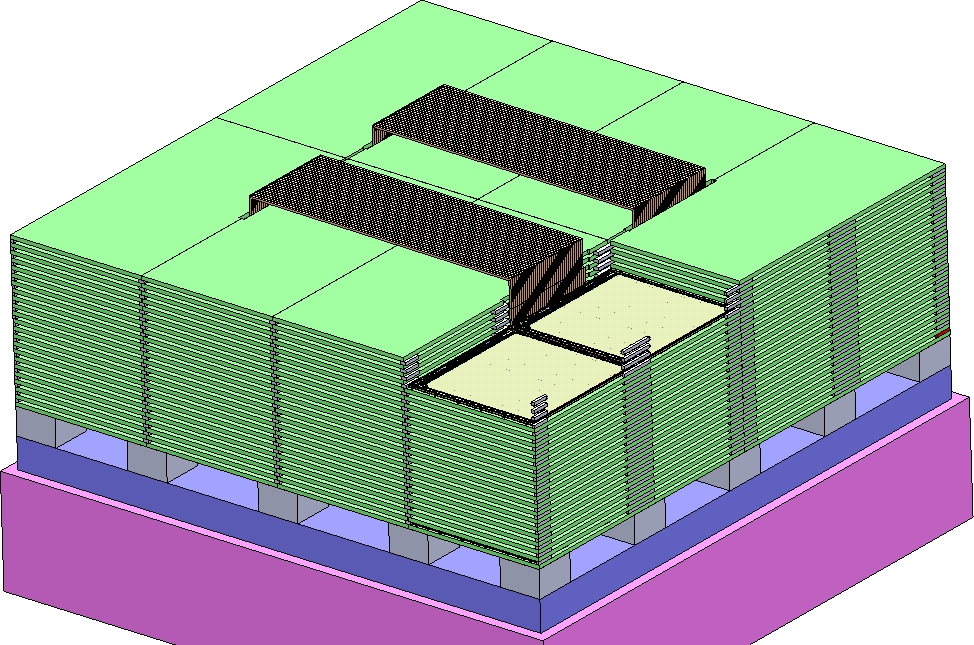
\includegraphics[width=0.6\linewidth]{engMod.png}
  \end{figure}
\end{frame}

\begin{frame}
  \frametitle{Engineering Module: Reconstruction}
  \vspace*{-9pt}
  \begin{figure}[h!]
    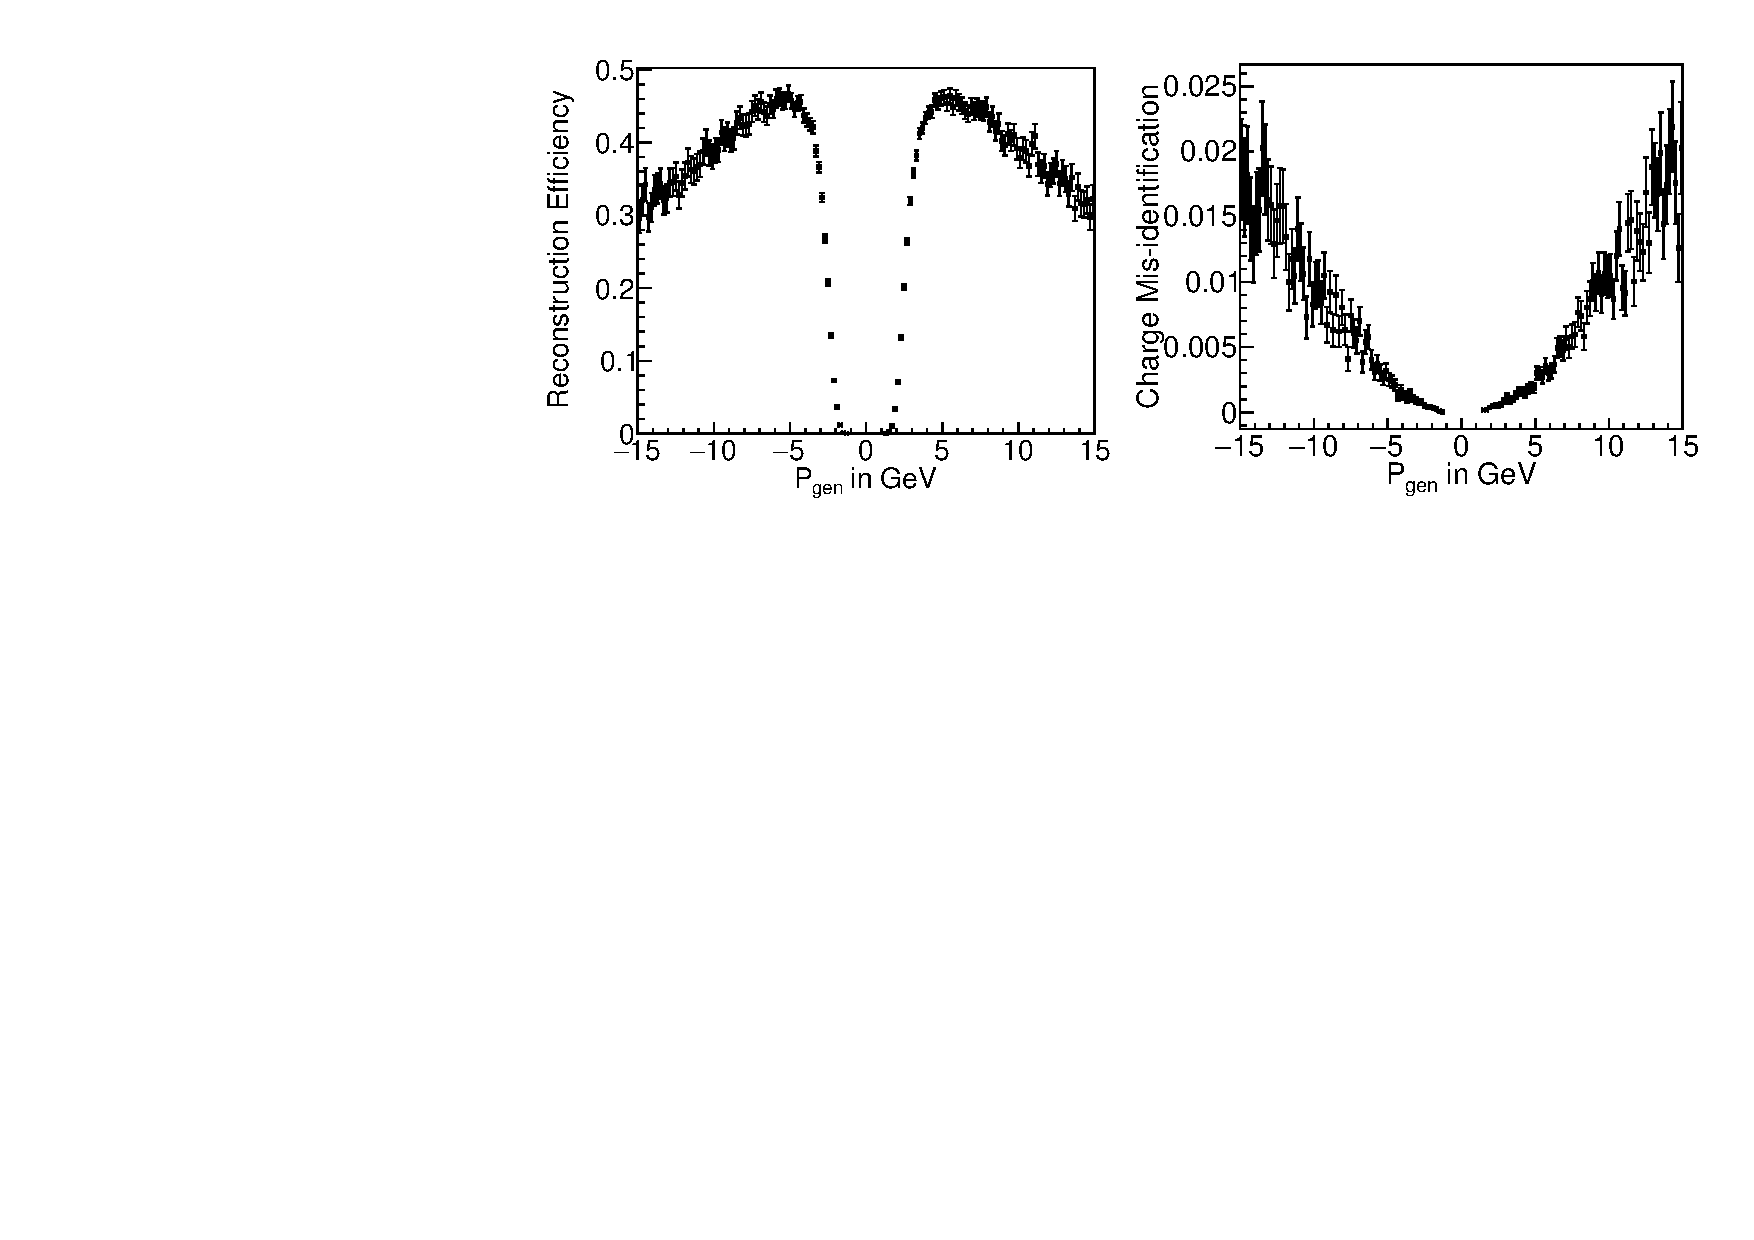
\includegraphics[width=0.7\linewidth]{GMA_effi_misId_20Layer_EM.pdf}
    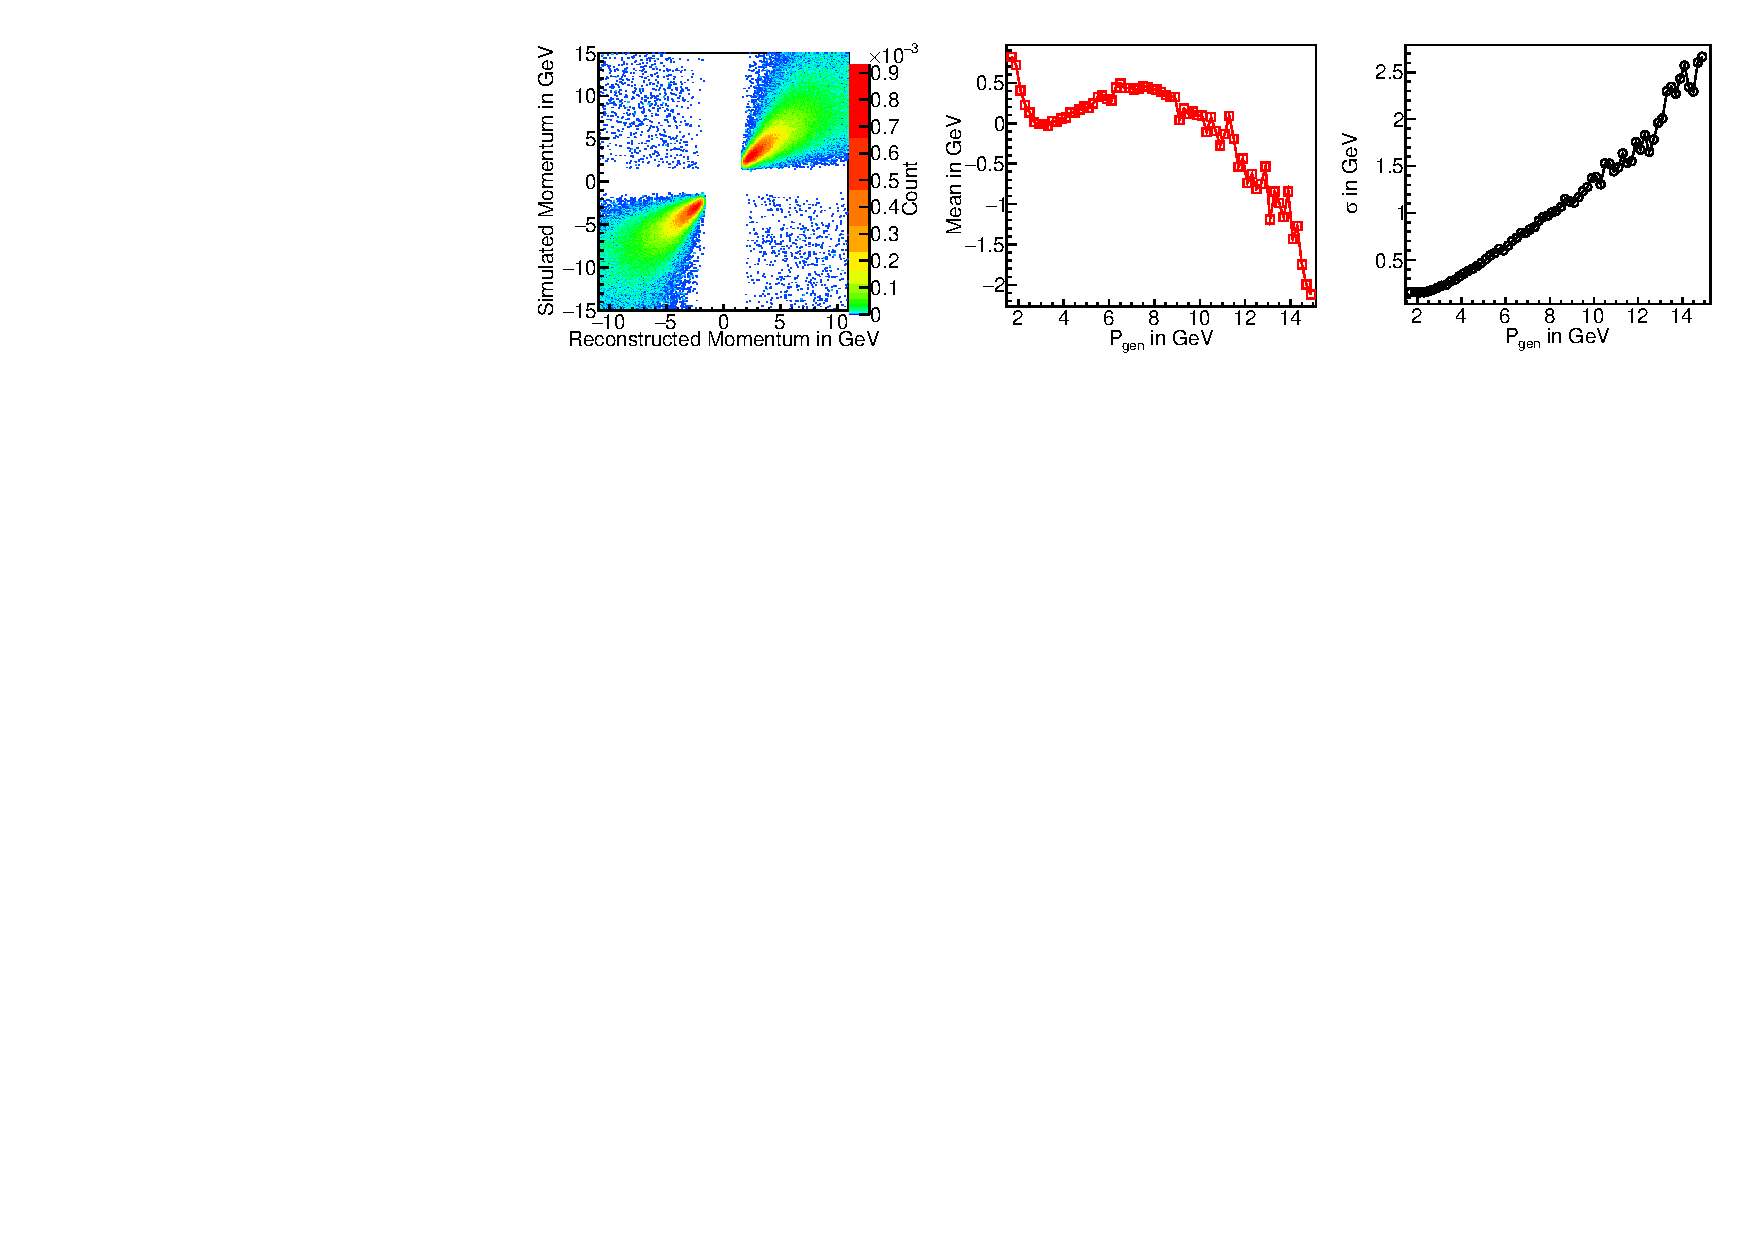
\includegraphics[width=1.\linewidth]{GMA_response_mean_sigma_20Layer_EM.pdf}
  \end{figure}
  \vspace*{-9pt}
  Momentum should be reconstructed up-to 12\,GeV
  with better charge identification and particle detection efficiency.
\end{frame}

\begin{frame}[shrink]
  \footnotesize{
    \colorbox{gray!40}{\begin{minipage}{1.0\textwidth}%% {17.5cm}
        \bf {Publications in peer-reviewed journals} 
    \end{minipage} }
    \begin{minipage}{1.10\textwidth}
      \begin{enumerate}
      \item {\bf S.~Mondal} et al. \textsc{Leak test of Resistive Plate Chamber gap by monitoring absolute pressure}, \textit{JINST} 14 (April 2019) P04009
      \item \textbf{S.~Mondal} et al. \textsc{Study of Particle Multiplicity of Cosmic Ray Events using 2\,m\,$\times$\,2\,m Resistive Plate Chamber Stack at IICHEP-Madurai}. \textit{Experimental Astronomy} (November 2020) 1--16
      \end{enumerate} 
    \end{minipage}
    %% \vspace{0.4cm}
    \colorbox{gray!40}{\begin{minipage}{1.0\textwidth}%% {17.5cm}
        \bf {Conferences/Workshops} 
    \end{minipage} }
    \begin{minipage}{1.10\textwidth}%% {1.05\textwidth}
      \begin{enumerate}
      \item Attended \emph{RPC2016} held at Ghent University during 22--26 February, 2016 \\
        {\bf{Poster:}} \textsc{Leak Rate Estimation of a Resistive Plate Chamber Gap by Monitoring Absolute Pressure}
      \item Attended \emph{XXII DAE-BRNS-HEP}  held at University of Delhi during 12-16 December, 2016 \\
        {\bf{Poster:}} \textsc{Estimation of Leak of a Resistive Plate Chamber by Monitoring Absolute Pressure}
      \item Attended \emph{NSPDI 2017} held at TIFR Mumbai during 4-7 October, 2017 \\
        {\bf{Poster:}} \textsc{Estimation of Leak of a Resistive Plate Chamber by Monitoring Absolute Pressure}
      \item Attended \emph{XXIII DAE-BRNS-HEP}  held at IIT Madras during 10-14 December, 2018 \\
        {\bf{Poster:}} \textsc{Muon Multiplicity in $2$\,m\,$\times$\,2\,m RPC and comparison with CORSIKA simulation}
      \item Attended \emph{XXIV DAE-BRNS-HEP}  held at NISER Bhubaneswar during 14-18 December, 2020 \\
        {\bf{Poster:}} \textsc{Correlation of muons arrival times from two different cosmic showers}\\
        {\bf{Talk:}} \textsc{Cosmic muon momentum spectra at Madurai}
      \end{enumerate}
    \end{minipage}
  }
\end{frame}

\begin{frame}
  \centering
  Thank You
\end{frame}

\end{document}
